\documentclass[journal]{IEEEtran}
\usepackage{amsmath,amssymb,amsfonts,graphicx,booktabs,array,cite,url}
\usepackage[hidelinks]{hyperref}
\newcommand{\func}[1]{\operatorname{#1}}
\newcommand{\col}{\operatorname{col}}
\newcommand{\tr}{\operatorname{tr}}
\newcommand{\dd}{\,\mathrm d}
\graphicspath{{figures/}}
\renewcommand{\thesection}{S\arabic{section}}
\renewcommand{\thesubsection}{\thesection.\arabic{subsection}}
\renewcommand{\theequation}{S\arabic{equation}}
\renewcommand{\thefigure}{S\arabic{figure}}
\renewcommand{\thetable}{S\arabic{table}}
\begin{document}
\title{Supplementary Material for\\``Implicit Representation Estimation, Prediction, and Control''}
\author{Mohamed Abdelghani}
\maketitle
\raggedbottom
\begin{abstract}
This companion documents the direct-partial learning studies in the main
paper and preserves earlier structured studies as separate supporting
records. The current Fourier, nonlinear contact, and Burgers experiments
adapt every field entry from observed incompatibility and use that same
field for readout. Section~\ref{sec:direct_main} gives their observation
boundaries, coupled updates, complete protocols, all-seed results, numerical
checks, and limitations. The Fourier benchmark tests independent prediction
with rapidly varying partials and slow supplied-input modulation. Contact
and Burgers test rate-level control with ideal rate sensing; approximate
contact recovery and failed causal/noisy Burgers cases are reported.
Sections S2--S18 retain coefficient-family protocols, comparisons, provenance,
and supporting examples. Their successful tasks do not establish direct
partial learning. Original missing archives and separately reproduced records
keep distinct identities. The enlarged flow views remain an unvalidated
legacy prototype. Section S19 distinguishes time derivatives from variations
of complete trajectories. Every formal result used by the main paper has
its complete proof there; the calculations here supply protocol details and
interpretation rather than replace those proofs.
\end{abstract}

\section{Scope, provenance, and reproducibility}
\label{sec:scope}
The current main evidence is in Section~\ref{sec:direct_main}: ten new
Fourier initializations/noise streams (seeds 10--19), five new contact
initializations (101--105), and the separately audited direct Burgers
ideal-sensing cohort (732--736). All declared seeds enter the summaries.
Figures use prospectively selected seeds 10, 101, and 732, respectively.
New protocols, pilot failures, and numerical refinements retain separate
identities. The Burgers records are reused without alteration; the main
figures are newly rendered from those records.

\subsection*{The direct-learning mechanism and its evidence}
All entries adapt from observed incompatibility $\widehat F(z)v$, without
fitting physical residual coefficients and differentiating them. The local
field uses the coupled normalized $Q,R$ flow; Fourier gives every partial
independent harmonic weights in the same flow on lifted rates. Constraint
count, context, units, memory, gain, and sensing remain supplied choices.
True partials and physical parameters belong to the simulator/evaluator,
not the learner or controller. Readouts use the learned field itself.
Normalization, observed compatibility, physical row-space recovery, and
successful task completion are separate checks.

Throughout, $F=D_zf$ denotes a physical Jacobian; a directly adapted field
need not itself be a globally integrable Jacobian. Gauge comparisons use
fixed context units. Inconsistent least squares depends on row weighting.
Initial levels needed by an integrated readout are measured separately.
Fourier's current graph benchmark demonstrates partial variation faster
than the actual supplied-input modulation, with known phase and order.
It does not inherit the earlier periodic dynamic plant's control claim.
Contact regulates vertical force rather than the earlier normal-force
magnitude. Burgers succeeds under ideal rate sensing while tested
causal/noisy alternatives fail; these are explicit limitations.

\subsection*{Retained structured studies and historical provenance}
Sections~\ref{sec:contact_protocol}, \ref{sec:fourier_protocol}, and
\ref{sec:burgers_protocol} document earlier prescribed-family studies.
Section~\ref{sec:normalized_fourier_results} retains the seven-coefficient
normalized periodic-plant experiment. Their coefficients induce evaluated
partials through supplied physical residual algebra; they are historical
comparisons, not the current direct-partial demonstrations.
Sections~\ref{sec:learning_rule_audit} and
\ref{sec:implementation_inventory} preserve their actual algorithms.
The earlier direct-lift diagnostics in Sections~\ref{sec:unanchored} and
\ref{sec:direct_lift_results} remain distinct from the new prediction test.

The retained structured records include 30 contact runs, 30 Burgers runs,
and 40 bounded-Fourier runs, with seeds 10--19 and the earlier seed-10
illustrations. Twenty paired contact-transfer runs are separate.
The normalized periodic study has ten controlled trajectories and ten
replay streams with same-stream shadow estimators. Contact was a disclosed
reconstruction; these newer experiments do not recover absent original
code or historical raw-record identities. Acrobot and active flow remain
structured supporting examples, and the ellipse is analytic only.

Section~\ref{sec:reproduction_audit} records a completed reproduction of
all 120 original structured/transfer protocols. Their regenerated archives
have their own checksums; the originally named historical archives remain
missing. The normalized periodic records have another protocol identity.
No earlier failure, guard, or unsuccessful sensing study is silently replaced
by the new main examples.

\subsection*{Reproduction files}
This supplement builds without private main-paper source or auxiliary files.
Current direct-study code and compact supporting records are under
\path{experiments/direct_submission/}; full raw records are identified by
the accompanying package manifest. The local submission package contains
source, configurations, seed lists, recorded outcomes, and checksums.
Legacy code and provenance remain in the repository. The project address is
\url{https://github.com/mnabdelghani/learning_implicit_representation}.
This address does not imply that the current local revision or its raw-data
archives have been published there. The accompanying versioned package,
not an assumed remote branch state, identifies this submission's evidence.
No archive DOI, publication acceptance, or open-source license is asserted.

\section{Sampled learning for the structured applications}
\label{sec:numerics}
This section applies to contact, Burgers, and the retained bounded Fourier
comparison. The retained normalized periodic-plant experiment uses
(\ref{eq:nf_coupled}) instead of the coefficient update below.
Let $\theta\in\mathbb R^p$ be scaled free coefficients. Supplied physical
terms are retained in a feature channel with fixed coefficient one:
\begin{equation}
 q_\theta=\col(\theta,1),\qquad \xi_{n,\ell}=q_\theta^{\mathsf T}v_{n,\ell}.
 \label{eq:sampled_implicit_relation}
\end{equation}
The fixed channel excludes the zero coefficient row. Here $v_{n,\ell}$ is a scaled observed feature row written as a column,
with $\ell$ indexing simultaneous equations or spatial samples; it need not
be the raw context rate $v=\dot z$ of the main paper. The column $q_\theta$
is the transpose of the experimental coefficient row $Q_\theta$ used there.
This coefficient row in feature coordinates is not the raw-context Jacobian
$F=D_zf$. The
experimental families also specify the zero residual level; differentiation
alone would not determine that level.

With sample interval $h$, memory time $\tau_m$, and
$\beta_m=\exp(-h/\tau_m)$,
\begin{align}
 R_n&=\beta_mR_{n-1}+(1-\beta_m)\langle v_nv_n^{\mathsf T}\rangle,
       &R_0&=0,\label{eq:discrete_memory}\\
 \mathcal J_n(\theta)&=\tfrac12q_\theta^{\mathsf T}R_nq_\theta.
 \label{eq:sampled_objective}
\end{align}
Brackets average simultaneous equations or spatial samples, not previously
fitted residuals. If $S=\col(I_p,0)$, the free gradient is
$G=S^{\mathsf T}R_nq_\theta$ and curvature is $H=S^{\mathsf T}R_nS$.
The implementation takes $M$ steps
\begin{equation}
 \theta^{j+1}=\Pi_{\mathcal W}(\theta^j-\alpha G(\theta^j)),\qquad
 \alpha=\{\max(\operatorname{tr}H,10^{-12})\}^{-1}.
 \label{eq:PG}
\end{equation}
For the declared box $\mathcal W$, this is a feasible descent step for the
\emph{fixed} memory problem because $\alpha\lambda_{\max}(H)\le1$.
Main-paper Proposition~6 (Descent of a sampled coefficient update) gives
\begin{equation}
 \mathcal J_n(\theta^{j+1})\le\mathcal J_n(\theta^j)
 -\|\theta^{j+1}-\theta^j\|^2/(2\alpha).
 \label{eq:discrete_descent}
\end{equation}
New observations change the objective; monotonically decreasing sample
energy along a noisy closed-loop trajectory is not promised.

At each decision time, available measurements and the pre-update model
select the next command. In contact, the current noisy force measurement
enters this readout before the commanded velocity is sampled; Fourier and
Burgers sample the noisy state rate after command selection. Partial and
incompatibility diagnostics use the pre-update coefficients, and only then
are the memory and coefficients updated. The already selected command is
held while the physical state advances by RK4. The final state is recorded,
but its unapplied command is excluded from task and effort statistics. The code never
feeds evaluator-only partials, clean rates, or true coefficients to an
adaptive update. Oracle branches deliberately use the true coefficients.
These evaluation windows retain online adaptation and overlapping
observations; pre-update scores are not independent held-out test errors.

As in the main paper, supplied and computed channels are roles in a current
query, not permanently measured and unmeasured variables. Observed history
trains the relation; a readout holds that estimate fixed and computes the
next command or a predicted rate from available data. The calibrated residual
families below allow direct commands. Predicting a future state from a rate
readout requires integration from known initial values. Instantaneous readout bounds do not
establish closed-loop stability or supply missing residual levels.

\subsection{Differential, gauge, and activity diagnostics}
For declared coordinate scales $D_z$ and row scales $D_r$, direct error is
\begin{equation}
 e_F=\frac{\|D_r(\widehat F-F)D_z\|_F}{\|D_rFD_z\|_F}.
\end{equation}
The fixed physical blocks select a common row convention. Contact and bounded Fourier
evaluate both differentials at the same clean simulator context to isolate
coefficient-induced error; these clean evaluator channels are not supplied to
the adaptive update. A complementary
basis-invariant diagnostic uses $A=FD_z$ and
\begin{equation}
 P_A=A^{\mathsf T}(AA^{\mathsf T})^{-1}A,\qquad
 e_P=\|P_{\widehat F D_z}-P_{FD_z}\|_F.
\end{equation}
QR bases compute these projectors without forming explicit inverses.
Burgers averages squared local projector distances over spatial sites before
taking a square root. Its direct error is the relative Frobenius norm after
stacking all spatial rows.

For an individual feature row, scale-normalized compatibility is
\begin{equation}
 \bar E_n=\frac{(q_\theta^{\mathsf T}v_n)^2}
 {\max(\|q_\theta\|^2\|v_n\|^2,10^{-20})}.
\end{equation}
Feature power $\|v_n\|^2$ is retained separately. A small normalized value
with sustained activity is more informative than raw energy alone, but
still does not certify identification of unexcited directions. Measured
memory eigenvalues include sensor noise; positivity in noisy data is not a
certificate of physical persistent excitation. True-model energy on the same
noisy observations is a reference, not an estimator-independent lower bound.

\section{Retained structured contact protocol}
\label{sec:contact_protocol}
\subsection{Plant, parameters, and observations}
The velocity-actuated contact plant is
\begin{align}
 \dot p&=Bu,\quad p=(x,y)^{\mathsf T},\quad d=h(x)-y,\\
 \tau_c\dot\lambda+\lambda&=k_c d+\eta_c\dot d,\quad
 h(x)=\gamma^{\mathsf T}\beta(x),\\
 \beta(x)&=(\sin 2x,\cos 5x)^{\mathsf T},\quad
 \gamma=(.035,.020)^{\mathsf T}.
\end{align}
The Cartesian reaction is $\ell=\lambda(-h'(x),1)^{\mathsf T}$ and the
controlled normal-force magnitude is $L=\|\ell\|$. Define
$a=k_c/\tau_c$, $b=\eta_c/\tau_c$, $\rho=1/\tau_c$,
$s=a\gamma$, and $r=b\gamma$.
Its material residual is
\begin{equation}
 f=\dot\lambda+\rho\lambda-s^{\mathsf T}\beta+ay
       -r^{\mathsf T}\beta'v_x+bv_y.
\end{equation} The parameters change at $60$ s:
\begin{equation}
 B_- =\begin{bmatrix}1&.15\\-.08&.85\end{bmatrix},\quad
 B_+ =\begin{bmatrix}.8&.22\\-.12&.65\end{bmatrix}.
\end{equation}
The respective $(k_c,\eta_c)$ are $(150,60)$ and $(250,90)$, while
$\tau_c=.25$ s remains known. The geometry is fixed. The full context is
$z=(x,y,\lambda,v_x,v_y,\dot\lambda,u_1,u_2)$. Its differential has the material row
\begin{equation}
 [\,-s^{\mathsf T}\beta'-r^{\mathsf T}\beta''v_x,\ a,\rho,
       -r^{\mathsf T}\beta',\ b,\ 1,\ 0,\ 0\,]
\end{equation}
and two kinematic rows whose
velocity block is $I_2$ and command block is $-B$.

Writing $c=(s_1,s_2,a,r_1,r_2,b)$, the newly declared prior is
$(8,4,400,3.2,1.6,160)$ and $\widehat B(0)=I_2$. The coefficient scales are
$(20,20,1000,10,10,300)$; lower bounds are
$(-100,-100,200,-50,-50,60)$ and upper bounds are
$(100,100,1600,50,50,700)$.
The diagonal entries of $\widehat B$ lie in $[.5,1.4]$ and off-diagonal
entries in $[-.3,.3]$. Consequently
$\det\widehat B\ge .5^2-.3^2=.16$ throughout adaptation. Both blocks use a 4-s memory and 48
projected steps per sample, unlike the earlier text's post-step clipping for
actuation. This implementation choice is disclosed rather than claimed to
reproduce an unavailable original script.

Initially $x=0$, $L=4$, and
$y=h(0)-\lambda/k_{c,-}$, where
$\lambda=4/\sqrt{1+h'(0)^2}$. The plant alone uses the true geometry and
material. Independent Gaussian force-component noise has standard deviation
$.01$ N and velocity noise $.001$ m/s; positions are exact. The force sensor
returns $\ell=\lambda(-h',1)^{\mathsf T}$ plus noise. The run lasts 120 s with
$h=.01$ s and an aligned change at $t=60$ s.

\subsection{Integral observations and fitted differential}
With $T=.1$ s, $I_g=\int_{t-T}^t g(\tau)\,d\tau$, and
$\Delta g=g(t)-g(t-T)$, the observed material incompatibility is
\begin{equation}
 \xi^I=\frac{\Delta\lambda+\rho I_\lambda
 -s^{\mathsf T}I_\beta+aI_y-r^{\mathsf T}\Delta\beta+b\Delta y}{T}.
 \label{eq:integral}
\end{equation}
It integrates the supplied material equation rather than differentiating
noisy force. The same candidate coefficients multiply all contributions in
each window. Trapezoids approximate the integrals. Exact integral
compatibility requires coefficients constant throughout the window;
change-crossing windows are retained and marked in the data. The reported
energy has units $\mathrm{N}^2/\mathrm{s}^2$.

The learner uses six free material channels
$(-I_{\beta_1},-I_{\beta_2},I_y,-\Delta\beta_1,-\Delta\beta_2,\Delta y)/T$
and the supplied channel $(\Delta\lambda+\rho I_\lambda)/T$.
Kinematics uses the simultaneous velocity residual $v_i-\widehat B_i u$.
The resulting fitted family is differentiated analytically to report the
raw-context $\widehat F$, including both $\beta'$ and $\beta''$ terms.
Thus low integral incompatibility is not mislabeled as a direct measurement
of $\widehat F\dot z$ in the raw context.

Direct-error diagnostics use
\begin{align*}
 D_z&=\operatorname{diag}(.5,.05,5,.3,.3,10,.5,.5),\\
 D_r&=\operatorname{diag}(.1,1/.3,1/.3).
\end{align*}
All physical partial entries are saved at $.1$-s intervals; learning remains
at $.01$ s. The reference energy recomputes the integral residual using the
true instantaneous coefficients on the same noisy samples, only in the
evaluator. Its change-crossing values need not vanish even without noise.

\subsection{Control readout}
The desired tasks are
\begin{align*}
 x_d&=.45\sin(.6t)+.08\sin(1.7t),\\
 L_d&=4+.7\sin(1.1t)+.4\sin(2.3t).
\end{align*}
Set $v_x^*=\dot x_d-4(x-x_d)$. If measured force is $\ell_m$,
$\lambda_m=(\ell_m)_y$ and $L_m=\|\ell_m\|$, the measured surface slope is
$\widehat h'_{\rm sens}=-(\ell_m)_x/\max(\lambda_m,.2)$.
Let $\widehat m=\sqrt{1+(\widehat h'_{\rm sens})^2}$ and
$\widehat h''=(\widehat s/\widehat a)^{\mathsf T}\beta''$.
The desired vertical-force rate is
\begin{equation}
 \dot\lambda^*=\frac{\dot L_d-20(L_m-L_d)
 -\lambda_m\widehat h'_{\rm sens}\widehat h''v_x^*/\widehat m}{\widehat m}.
\end{equation}
The material readout yields
\begin{equation}
 v_y^*=\frac{\widehat s^{\mathsf T}\beta-\widehat a y-\rho\lambda_m
 +\widehat r^{\mathsf T}\beta'v_x^*-\dot\lambda^*}{\widehat b}.
\end{equation}
Finally $u=\operatorname{clip}_{[-.8,.8]}\{\widehat B^{-1}(v_x^*,v_y^*)^{\mathsf T}\}$.
Measured direction, fitted curvature, and learned dynamics are used; true
surface derivatives are not available to the adaptive controller.
The oracle uses the true coefficients but the same noisy force sensor.
The frozen controller uses the same initial model and outer gains.

\section{Retained bounded Fourier Memory comparison}
\label{sec:fourier_protocol}
This original six-coefficient protocol is retained as a representation and
structured-update comparison. It does not generate the revised main Fourier
figure, whose direct graph protocol is documented in
Section~\ref{sec:direct_main}. Section~\ref{sec:normalized_fourier_results}
retains the later normalized periodic-plant comparison.
The periodic implicit plant is
\begin{align}
 f&=\rho(\phi)\dot x+\kappa(\phi)x-u=0,\quad \phi=4t,\\
 \rho&=1.20+.27\cos\phi-.18\sin\phi,\\
 \kappa&=1.50+.34\cos\phi+.24\sin\phi.
\end{align}
The prior coefficients are $(1,0,0,1,0,0)$. The context
$z=(x,\dot x,u,\phi)$ gives
\begin{equation}
 F=[\,\kappa,\rho,-1,\rho'\dot x+\kappa'x\,].
\end{equation}
Coefficient lower and upper bounds are
$(1,-.3,-.3,.8,-.5,-.5)$ and $(1.6,.3,.3,2.2,.5,.5)$, with scales
$(1,.3,.3,1,.4,.4)$. The resulting positive rate block is certified for all
phases. The $K=0$ model uses the constant entries with the same associated
bounds and scales, setting all harmonic entries to zero.

With $\varphi=\col(1,\cos\phi,\sin\phi)$ and primes denoting
phase derivatives, define $\zeta=\col(\varphi\dot x,\varphi x,-u)$.
Causal complete-feature secants are
$[\zeta(t)-\zeta(t-.05)]/.05$; the current candidate is used for both
endpoints. In particular,
$d(\dot x\cos\phi)/dt=\ddot x\cos\phi-\dot x\dot\phi\sin\phi$.
The coefficient-induced Jacobian therefore contains the full clock partial, rather than
omitting this chain-rule term. The secants are sampled endpoint constraints,
not exact instantaneous derivatives across command changes. The displayed
clock partial differentiates with respect to phase $\phi$, not time $t$.

The initial state is $x(0)=.2$. The input computed from the pre-update model
is held during each $.01$-s RK4 step, while $\phi=4t$ advances at the RK4
stage times. The supplied state, input, and phase are exact; only the observed
state rate receives independent Gaussian noise of standard deviation $.001$.
The run lasts 80 s, with an 8-s memory and eight projected steps per sample.
The control readout is
\begin{equation}
 u=\widehat\rho[\dot x_d-2(x-x_d)]+\widehat\kappa x,
 \quad x_d=.45\sin(.7t)+.2\sin(1.3t).
 \label{eq:fourier_control}
\end{equation}
Input amplitude is unrestricted. All methods use the same reference,
feedback gain, state initialization, and sample rate. Noise has no effect on
the frozen/oracle control command because those branches do not adapt and
their state measurement is exact; their tracking dispersion is therefore zero.

A $K=0$ \emph{shadow} update uses the $K=1$ learner's very same observed
features but never controls that plant. Its energy comparison isolates
representation on common data. A distinct $K=0$ \emph{control} branch
learns on its own trajectory and supplies the task-RMSE comparison. These
are different comparisons and must not be conflated. Frequency
identification is not tested: phase and harmonic order are
supplied, and both learners use the same exponential memory time. Direct differential
error uses $D_z=\operatorname{diag}(.5,1,1,1)$ and $D_r=1$; coefficient
error is the Euclidean relative error of the six physical coefficients.

Figure~\ref{fig:fourier_bounded} shows the rate and clock partials over the initial 16 s to
make the rapid variation readable. Complete trajectories remain in the
recorded traces. The mean measured energy of the learned model can be
slightly below the same-stream true-model value because noisy features bias
an energy minimizer; this is not evidence that the fitted model is more
physically correct than the true model.

For $60\le t<80$~s, ten-seed mean incompatibility on the common learned
stream is $5.9603\times10^{-4}$ for the $K=1$ estimate,
$8.7874\times10^{-2}$ for its $K=0$ shadow, and
$5.9712\times10^{-4}$ for the evaluator-only true model. The separate
$K=1$ and $K=0$ controllers have tracking RMSE
$0.002299\pm0.000031$ and $0.047928\pm0.000011$, respectively;
the oracle value is $0.001229$. These values come from the original
\path{results/aggregate.json}. The omitted-harmonics comparison tests
representation capacity with known phase, not frequency discovery or an
advantage over an equally expressive periodic model. Matched-family
estimator comparisons appear in Section~\ref{sec:estimator_comparison}.

\begin{figure*}[t]
\centering
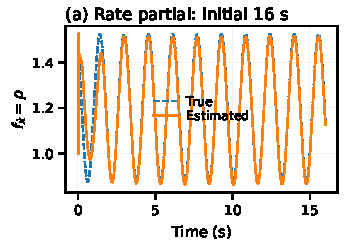
\includegraphics[width=.325\textwidth]{fourier_partial_rate.pdf}\hfill
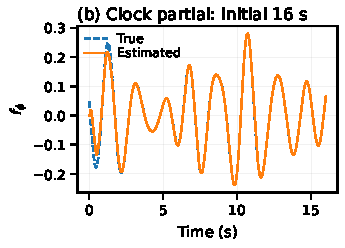
\includegraphics[width=.325\textwidth]{fourier_partial_phase.pdf}\hfill
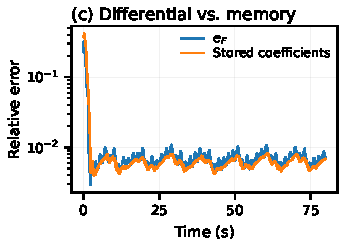
\includegraphics[width=.325\textwidth]{fourier_F_error.pdf}\\
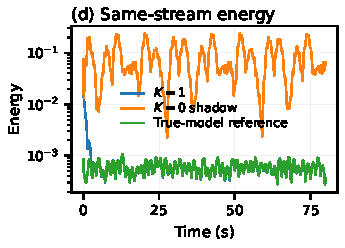
\includegraphics[width=.325\textwidth]{fourier_energy.pdf}\hfill
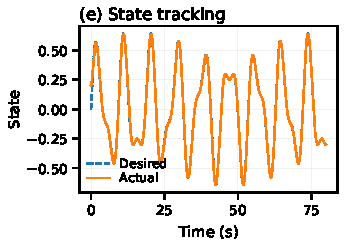
\includegraphics[width=.325\textwidth]{fourier_task.pdf}\hfill
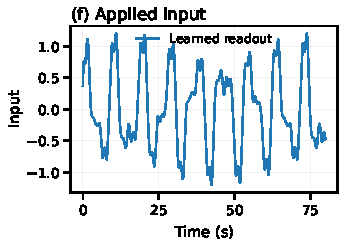
\includegraphics[width=.325\textwidth]{fourier_control.pdf}
\caption{Original bounded Fourier comparison, preselected seed 10. Upper
row: evaluated rate and phase partials during the first 16 s, then full-run
differential and coefficient errors. Lower row: incompatibility of the
learned model, its same-stream $K=0$ shadow, and the true-model reference;
state tracking; applied command. Only the energy panel uses a causal
one-second mean. The six adaptive coefficients determine the varying
partials, including both phase-product terms; the input partial is supplied.
These unchanged records use the box-projected update, independently of the
retained normalized periodic-plant experiment.}
\label{fig:fourier_bounded}
\end{figure*}

\section{Retained structured Burgers protocol}
\label{sec:burgers_protocol}
The supplied reconstruction is reused without changing its plant, learner,
or controller. On the periodic domain $s\in[0,2\pi)$ its residual is
\begin{equation}
 f=w_t+c_a w w_s-\nu w_{ss}-bu=0.
\end{equation}
For $z=(w,w_s,w_{ss},u,w_t)$,
$F=[c_a w_s,c_a w,-\nu,-b,1]$.
The desired field is
$w_d=.4\sin s\cos(.7t)+.2\cos(2s)\sin(1.1t)$, the initial field is
$.3\sin s+.1\cos(2s)$, and the controller uses
$u=((w_d)_t+\hat c_a w w_s-\hat\nu w_{ss}-2(w-w_d))/\hat b$.
The run lasts 24 s, uses a $.005$-s step, a 4-s memory, eight inner steps,
and independent rate noise of standard deviation $.002$. It uses a 64-point periodic Fourier collocation grid, pointwise
$ww_s$, and no extra dealiasing filter. The same spatial operators form the
plant and residual features. True coefficients are $(1,.08,1)$ and the prior
is $(.7,.04,.8)$. Scales are $(1,.1,1)$, with lower bounds $(.2,.01,.25)$ and
upper bounds $(2,.25,2)$. The positive input block makes the specified inverse
readout feasible throughout learning. Input is unconstrained at every grid
site; no sparse-actuator or sparse-sensor claim is made.

The learner differences the complete features $(w_t,ww_s,-w_{ss},-u)$
over $.05$ s and accumulates spatially averaged correlations. The $w_t$
coefficient is fixed at one. For independent rate-noise samples of variance
$\sigma^2$, the true-model half-squared secant residual has expectation
$\sigma^2/T^2=.0016$. Overlapping windows produce temporal dependence, so
individual points are not treated as independent statistical replicates.
Between-seed summaries use independently generated sensor noise.

The displayed raw-context partials are evaluated on the same measured field
for true and estimated coefficients. $D_z=I_5$, $D_r=1$; the state and its
spectral derivatives are exact in this setup. Selected-site plots use
$s=\pi/2$, fixed before execution. The complete field, desired field,
applied control, and predicted/true rates are saved every $.1$ s, while
learning occurs every $.005$ s. The terminal unapplied command is excluded
from the $[18,24)$-s evaluation interval.

\section{Extended diagnostic figures}
\label{sec:diagnostics}
Figures~\ref{fig:contact_fourier_diagnostics} and~\ref{fig:burgers_diagnostics}
extend the contact, retained bounded-Fourier, and Burgers diagnostics.
Table~\ref{tab:main_results} reports the original 100 structured-protocol
runs; the normalized Fourier results are in
Table~\ref{tab:normalized_fourier_results}. Panels are described in reading order.
\begin{figure*}[t]
\centering
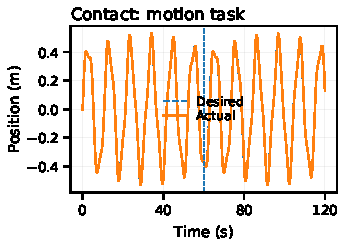
\includegraphics[width=.325\textwidth]{contact_motion.pdf}\hfill
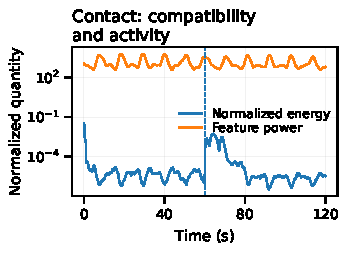
\includegraphics[width=.325\textwidth]{contact_activity.pdf}\hfill
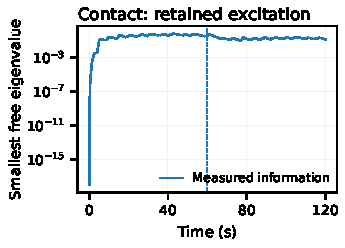
\includegraphics[width=.325\textwidth]{contact_information.pdf}\\
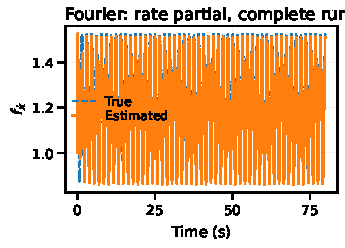
\includegraphics[width=.325\textwidth]{fourier_full_partial.pdf}\hfill
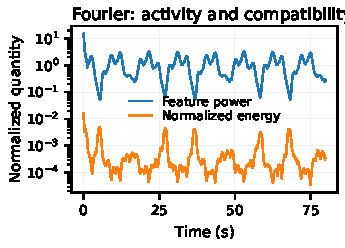
\includegraphics[width=.325\textwidth]{fourier_activity.pdf}\hfill
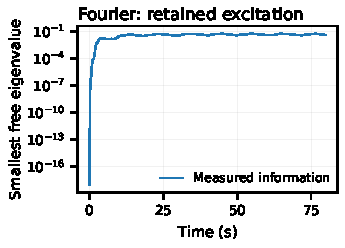
\includegraphics[width=.325\textwidth]{fourier_information.pdf}
\caption{Additional contact and bounded-Fourier diagnostics, seed 10. Top row,
left to right: contact motion, feature activity, and memory spectrum. Bottom
row: Fourier rate partial, feature activity, and memory spectrum. Motion remains
active while compatibility improves; a small residual is not explained solely
by stopping the system. The information spectra are empirical diagnostics
of noisy feature memory, not certificates of noise-free persistent excitation.
The Fourier rate partial is shown over the complete run.}
\label{fig:contact_fourier_diagnostics}
\end{figure*}
\begin{figure*}[t]
\centering
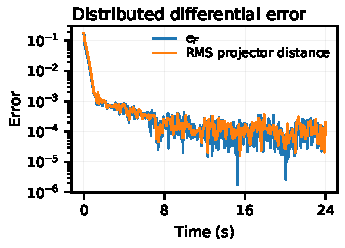
\includegraphics[width=.325\textwidth]{burgers_F_error.pdf}\hfill
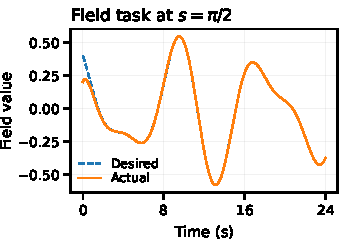
\includegraphics[width=.325\textwidth]{burgers_task.pdf}\hfill
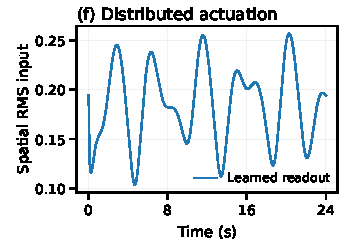
\includegraphics[width=.325\textwidth]{burgers_control.pdf}
\caption{Retained structured Burgers diagnostics, seed 10.
Left to right: full
spatial differential error, actual versus desired field at $s=\pi/2$, and
applied distributed control effort.}
\label{fig:burgers_diagnostics}
\end{figure*}
\begin{table*}[t]
\centering
\caption{New main-paper runs: ten noise seeds per method. Contact task errors are force RMSE in N over $[100,120)$ s; Fourier errors are state RMSE over $[60,80)$ s; Burgers errors are spatial--temporal RMS over $[18,24)$ s. These metrics have different units and are not compared across systems.}
\begin{tabular}{llrr}
\toprule Study & Method & Task RMS (mean $\pm$ SD) & Mean scaled $e_F$ ($\pm$ SD) \\
\midrule
Contact & learned & $0.00342486\,\pm\,0.00018$ & $0.000895904\,\pm\,0.00043$ \\
Contact & frozen & $0.855492\,\pm\,0.00027$ & $0.583578\,\pm\,3.2\times10^{-8}$ \\
Contact & oracle & $0.0032347\,\pm\,0.00013$ & $0\,\pm\,0$ \\
Fourier & learned & $0.00229896\,\pm\,3.1\times10^{-5}$ & $0.00687125\,\pm\,0.00019$ \\
Fourier & K0 & $0.0479282\,\pm\,1.1\times10^{-5}$ & $0.184933\,\pm\,8.6\times10^{-6}$ \\
Fourier & frozen & $0.0672733\,\pm\,0$ & $0.214235\,\pm\,2.9\times10^{-17}$ \\
Fourier & oracle & $0.00122862\,\pm\,0$ & $0\,\pm\,0$ \\
Burgers & learned & $0.000197473\,\pm\,1.9\times10^{-6}$ & $0.000107351\,\pm\,1.1\times10^{-5}$ \\
Burgers & frozen & $0.0165846\,\pm\,3.7\times10^{-18}$ & $0.158437\,\pm\,2.9\times10^{-17}$ \\
Burgers & oracle & $0.000197656\,\pm\,2.9\times10^{-20}$ & $0\,\pm\,0$ \\
\bottomrule
\end{tabular}
\label{tab:main_results}
\end{table*}


\section{Interpreting the theory and retained protocols}
\label{sec:interpretation}
All results used by the main paper retain their complete proofs there. The references below
use its theorem and proposition numbers; equations numbered with an S
belong to this supplement. These notes explain the limits of applying the
results to the protocols. Additional supporting implementation proofs appear
in Section~\ref{sec:learning_rule_audit}.

\subsection{Feasible descent and stationary exceptions}
Main-paper Propositions~1--2 (Row-Stiefel projected gradient flow and
Single-sample convergence) give feasibility, fixed-sample descent, and the
required initialization condition. If the observed rate lies in the current
row space, the sample update can be stationary with nonzero incompatibility.
Main-paper Proposition~6 justifies the fixed-memory coefficient step in
(\ref{eq:PG})--(\ref{eq:discrete_descent}). Changing observations need not
produce monotonically decreasing measured energy. The retained structured contact, Burgers, and bounded Fourier comparisons
use fixed physical channels and coefficient boxes. The retained normalized
periodic study integrates the coupled law in seven physical-feature
coordinates; its complete-feature secants differ from raw-context tangents.
The current direct studies in Section~\ref{sec:direct_main} instead adapt
every local entry or independent harmonic field weight.

\subsection{Identification and local tracking}
Main-paper Propositions~3--4 distinguish a covariance minimizer from the
physical row space: exact identification requires one shared differential
compatible with the retained history and excitation on its kernel.
Theorems~1--2 require the stated nonzero or invertible projection of the
initial estimate onto the target space. Nonglobal invariant eigenspaces
can otherwise be stationary despite descent.

Theorem~3 is local: it requires a separating gap
$\lambda_{m+1}(R)-\lambda_m(R)\ge\mu>0$, slow covariance drift, and
initialization inside its invariant attraction neighborhood. Positivity of
$\lambda_{m+1}$ alone is insufficient when $\lambda_m>0$.
Proposition~5 separates tracking of the covariance eigenspace from bias
relative to the physical differential. Neither noisy memory eigenvalues
nor good task performance establish these hypotheses.

\subsection{Readouts and Fourier Memory}
Main-paper Theorem~4 and Proposition~7 bound instantaneous errors of regular
readouts, in a common row convention or through normalized-row projectors,
respectively. They do not imply closed-loop stability. Proposition~8 concerns
the unguarded lifted covariance problem; phase coverage and coefficient
normalization alone do not ensure coefficient identification or phasewise
nondegeneracy. The main paper supplies the phase guard and the Fourier
normal-equation mismatch bound. Section~\ref{sec:unanchored} retains the
separate anchor-free reconstruction. Both retained Fourier plant protocols use
complete harmonic--state feature secants and report the full clock partial;
their coefficient constraints and optimizers differ.

\subsection{Compatibility without complete identification}
Nonvanishing activity does not ensure that every partial is identified.
For example, $F=(1,1,-1)$ and $\widehat F=(1,5,-1)$ both annihilate
$v=(1,0,1)^{\mathsf T}$, which is nonzero. Both support the task readout
$v_3=v_1$ when the second channel is held fixed, but disagree on perturbations
of that second channel. The fixed last coefficient excludes collapse;
normalized incompatibility is still zero along this trajectory. This
algebraic example separates task-relevant compatibility from complete
identification without relying on vanishing context rates. It does not
establish a general nonlinear closed-loop theorem.

Section~\ref{sec:trajectory_variations} compares temporal excitation with
whole-trajectory variations and analyzes the periodic context's kinematic
ambiguity.

\section{Supplementary study: task-only interaction versus bounded excitation}
\label{sec:excitation}
This supplementary experiment is separate from the original 100 structured
protocol runs and the retained normalized Fourier experiment. It is a
historical coefficient-based study, separate from the current direct-field
main evidence in Section~\ref{sec:direct_main}. It examines whether a small incompatibility and accurate
regulation necessarily imply accurate evaluated partials within a prescribed
residual family. The learner itself is the retained coefficient estimator,
not a direct all-entry partial-field learner.
The same viscoelastic contact plant and initial parameter prior are used in
both protocols, without the material or actuation change. All remaining plant, noise,
memory, bounds, and sampling settings are those in
Section~\ref{sec:contact_protocol}. During $0\le t<60$~s the
reference is $x_d=0$, $L_d=4$~N. The task-only controller performs regulation
without deliberately exciting the system. The probing controller adds to
its calculated command the bounded deterministic signal
\begin{align}
 p_1(t)&=.08\{\sin(.7t)+.5\sin(1.9t+.3)\},\\
 p_2(t)&=\frac{.02}{1.5}\{\sin(1.1t+.5)+.5\sin(2.7t)\}.
\end{align}
The resulting command is subject to the same $\pm.8$ componentwise limits.
The same ten measurement-noise seeds (10--19) are used. At $t=60$~s,
learning and probing stop, the estimates are frozen, and both controllers
receive the previously defined oscillatory contact-force and motion task
with the reference clock reset. The transfer evaluation is $[70,80)$~s.
Thus the test distinguishes performance on the task generating training data
from reuse on a new task; it is not an assertion of safe exploration.

The held-out diagnostic uses the frozen estimate at $t=60$~s on 1000
common evaluator-only contexts: $x$ and $v_x$ are independently uniform on
$[-.5,.5]$, generated with random seed 2026; the other context entries are
zero. It reports the square root of the summed squared scaled differential
errors divided by the summed squared scaled true differentials, using the
same $D_z,D_r$ as the contact protocol. These queries are algebraic contexts,
not additional plant trajectories, and never train either learner.
Table~\ref{tab:excitation} and Figure~\ref{fig:excitation} give the results.

\begin{table}[t]
\centering
\caption{Paired excitation experiment, mean $\pm$ sample SD over ten seeds.
Training is $[40,60)$~s; transfer is $[70,80)$~s.}
\setlength{\tabcolsep}{5pt}
\begin{tabular}{lcc}
\toprule Quantity & Task only & Bounded probing\\
\midrule
Training force RMSE (N) & $0.00261\pm0.00011$ & $0.16407\pm0.00238$\\
Training $e_F$ & $0.19252\pm0.00606$ & $0.01904\pm0.00257$\\
Transfer force RMSE (N) & $0.98558\pm0.28077$ & $0.06501\pm0.00511$\\
Held-out $e_F$ & $0.19596\pm0.00802$ & $0.04232\pm0.00203$\\
\bottomrule
\end{tabular}
\label{tab:excitation}
\end{table}
\begin{figure*}[t]
\centering
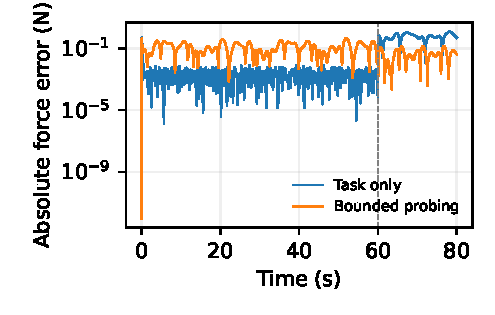
\includegraphics[width=.32\textwidth]{excitation_force.pdf}\hfill
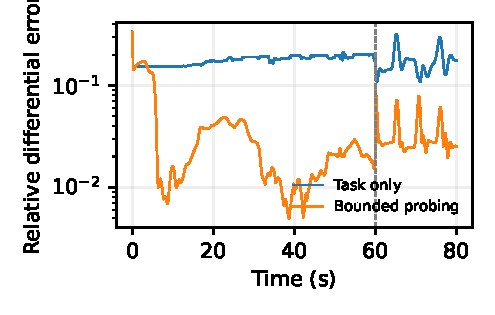
\includegraphics[width=.32\textwidth]{excitation_partial.pdf}\hfill
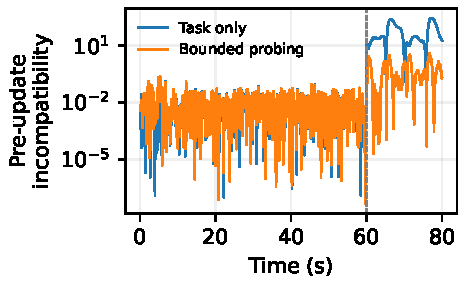
\includegraphics[width=.32\textwidth]{excitation_energy.pdf}\\
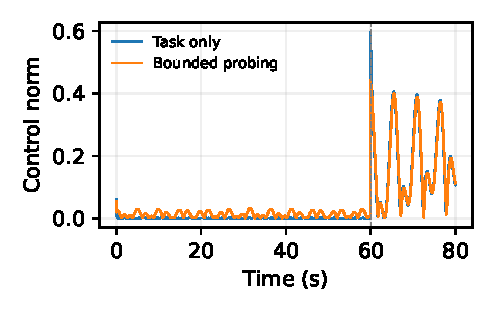
\includegraphics[width=.32\textwidth]{excitation_control.pdf}\hfill
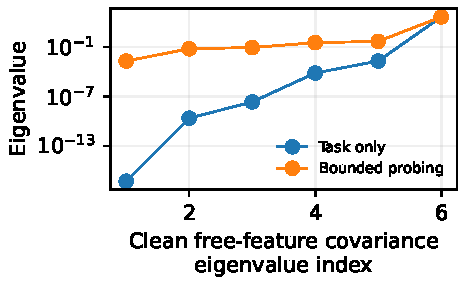
\includegraphics[width=.32\textwidth]{excitation_information.pdf}
\caption{Paired excitation. The trajectory panels show preselected seed 10.
Top row, left to right: force error,
relative differential error, and pre-update incompatibility. Bottom row:
applied command and the clean evaluator-only
information spectrum at the end of training, averaged over all ten seeds.
The vertical line marks
transfer to a new task with coefficients frozen. Clean information is not
provided to either learner.}
\label{fig:excitation}
\end{figure*}

The task-only controller maintains near-perfect regulation with negligible
control activity, and its incompatibility approaches the same-stream
true-model reference. Nevertheless its differential error remains substantial,
and its frozen model transfers poorly. The bounded probe incurs a training
tracking cost but yields substantially improved partial estimation and
transfer performance. These are illustrative outcomes for this specific
prescribed feature family and excitation signal; they do not imply a general
necessity or sufficiency theorem for task-specific learning.


\section{Additional worked constructions}
\label{sec:constructions}
These mechanical and geometric examples expand the main paper's distinction
between direct rate-product relations and Jacobian-derived differentials.
\subsection{Nonlinear mechanical dynamics}
The direct rate-product construction is especially natural for mechanical
systems. A robot with joint positions $q$, velocities $w=\dot q$, joint
torques $\tau_m$, and an external contact wrench $\lambda$ obeys, on a
smooth interval without impacts, 
\begin{equation}
M(q)\ddot q+C(q,\dot q)\dot q+G(q) =\tau_m+J_c(q)^{\mathsf{T}}\lambda.
\label{eq:mechanical}
\end{equation}
The inertia matrix $M(q)$ couples joint accelerations, the term $C(q,w)w$
describes velocity-dependent forces, $G(q)$ accounts for gravity, and the
contact Jacobian $J_c(q)$ maps the external wrench into generalized joint
forces. A command $u$ produces torque $\tau_m=B(q)u$, where the actuation
matrix $B(q)$ need not be square; for direct torque actuation $B=I$. Write $%
h(q,w)=C(q,w)w+G(q)$. The force balance is then 
\begin{equation}
M(q)\dot w+h(q,w)-B(q)u-J_c(q)^{\mathsf{T}}\lambda=0.
\label{eq:mechanical_balance}
\end{equation}

To express this balance in terms of context rates, retain $q$ and $w$ and
add the integrated command $s_u$, integrated contact wrench $s_\lambda$, and
clock coordinate $r_0$ defined by $\dot s_u=u$, $\dot s_\lambda=\lambda$,
and $\dot r_0=1$. For the resulting context 
\begin{equation}
z=\func{col}(q,w,s_u,s_\lambda,r_0),  \label{eq:mechanical_context}
\end{equation}
the observed or estimated rates are 
\begin{equation}
\dot z=\func{col}(w,\dot w,u,\lambda,1).  \label{eq:mechanical_rates}
\end{equation}
We now collect the coefficients of these rates, in the same order, into the
matrix-valued function 
\begin{equation}
H(z)=%
\begin{bmatrix}
0 & M(q) & -B(q) & -J_c(q)^{\mathsf{T}} & h(q,w)%
\end{bmatrix}%
.  \label{eq:mechanical_coefficients}
\end{equation}
The original equations of motion are therefore exactly 
\begin{equation}
H(z)\dot z=0.  \label{eq:mechanical_product}
\end{equation}
The symbol $H$ denotes the coefficient matrix assembled from the physical
equations; it is not introduced as the derivative of an unknown function. In
general it need not equal a Jacobian $D_zf$: such an equality would require
the additional integrability conditions on its entries. Nevertheless, the
rate-product equation in (\ref{eq:mechanical_product}) supplies a
differential compatibility relation directly, without differentiating the
force balance in (\ref{eq:mechanical_balance}). For the learning agent, the
mechanics and their coefficient blocks may be unknown; the measured motion
and commanded inputs provide the variations from which a compatible relation
can be estimated. Contact forces must themselves be measured or estimated if
they are to enter the chosen context. The additional Acrobot example below uses a prescribed mechanical family.


\subsection{Geometric constraints}
The preceding examples already contain rates in their governing equations. A
geometric constraint shows why differentiation is sometimes needed to obtain
a differential representation. A point moving on a circle of radius $R$
obeys 
\begin{equation}
f(x,y)=x^2+y^2-R^2=0.  \label{eq:circular_constraint}
\end{equation}
This equation relates positions but contains no motion rates.
Differentiating it along any differentiable admissible path gives 
\begin{equation}
2x\dot x+2y\dot y=0.  \label{eq:circular_differential}
\end{equation}
Thus, with $z=\func{col}(x,y)$, the coefficient field is indeed the Jacobian
of the constraint: 
\begin{equation}
F(z)=D_zf(z)=%
\begin{bmatrix}
2x & 2y%
\end{bmatrix}%
,  \label{eq:circular_jacobian}
\end{equation}
and the differential representation is $F(z)\dot z=0$. The distinction from
the mechanical example is now explicit: $F$ is obtained by differentiating $%
f $, whereas $H$ was read directly from the force balance. Moreover, the
differential field in (\ref{eq:circular_jacobian}) contains no information
about $R$. Zero incompatibility can identify a relationship consistent with
observed motion without identifying the particular level set; an observed
initial position supplies the missing radius.



\section{Anchor-free Fourier diagnostic}
\label{sec:unanchored}
An exact scalar example illustrates the lift without fixing any coordinate
of the differential. Let $f(x,y)=y+\sin x=0$ and $z(t)=(t,-\sin t)^{\mathsf{T%
}}$. Then $v=(1,-\cos t)^{\mathsf{T}}$ and $F(t)=(\cos t,1)$. A constant
unmodulated row cannot annihilate every observed velocity, since $%
\int_0^{2\pi}vv^{\mathsf{T}}\,\,\mathrm{d} t =\func{diag}(2\pi,\pi)$. For $%
K=1$, a unit-norm stored row 
\begin{equation}
C_\star=\frac1{\sqrt2}(0,1,\ 1,0,\ 0,0)  \label{eq:fourier_example}
\end{equation}
annihilates $w=\col(v,\cos t\,v,\sin t\,v)$ at every time. Here the lifted
covariance has exactly one zero eigenvalue and a positive gap. Its evaluated
row is $C_\star\Psi_1(t)=(\cos t,1)/\sqrt2$, whose Euclidean norm is at
least $1/\sqrt2$ at all phases. The retained diagnostic reports recovery without selecting a privileged
derivative block. The original report used 4096 rates over a cycle and
1600 retracted gradient steps. The reported
final row-space error is below $10^{-7}$; the phase-grid minimum of the
evaluated row norm is $.7071$. The exact target has the analytic bound $%
1/\sqrt2$; the finite-grid guard used during learning is not a continuum
certificate for arbitrary coefficients. The figure and reported values are
retained, but the standalone generating script and underlying iteration
records are absent from the supplied repository. These numerical values
have therefore not been independently reproduced from the supplied artifacts.
\begin{figure}[t]
\centering
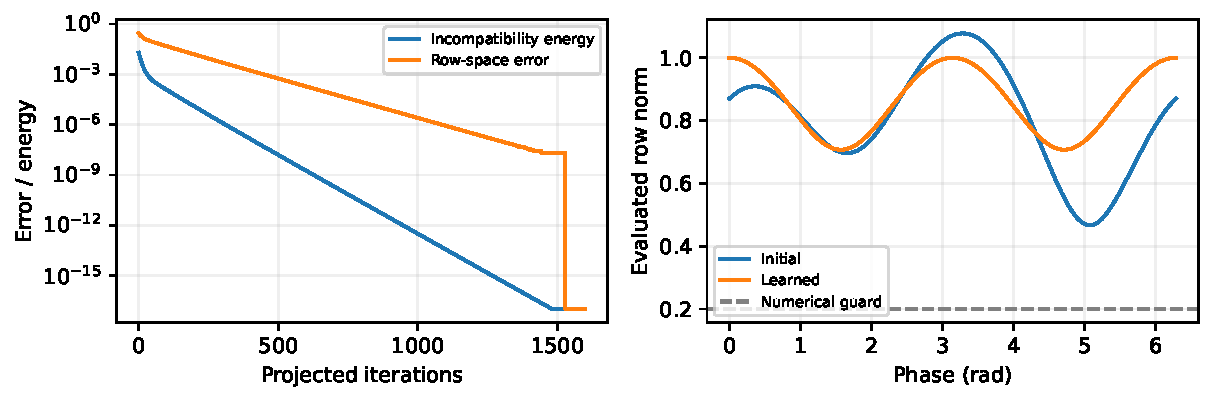
\includegraphics[width=.95\columnwidth]{figures/unanchored_fourier}
\caption{Unanchored Fourier example: the row-Stiefel constrained learner
minimizes accumulated incompatibility and recovers the one-dimensional row
space. This retained plot is independent of the main experiments; its standalone
generating script and iteration records were not supplied.}
\label{fig:unanchored_fourier}
\end{figure}



\section{Additional examples retained with the code}
\label{sec:additional_examples}
The Acrobot and flow figures retain their original archival titles. In those
titles, ``new reconstruction'' and ``new flow prototype'' refer to the
previously supplied studies, not to the main-paper runs.
\subsection{Acrobot: offline initialization and later control}
The supplied reconstruction uses the mechanical family
\begin{equation}
 f_c=M_c(q)\ddot q+h_c(q,\dot q)-(0,u)^{\mathsf T}=0,
\end{equation}
with five coefficients and a known actuator location. Coefficient learning
uses causal complete-feature differences during an 8-s excitation episode;
partials are then evaluated from the supplied mechanical family.
The final model is then queried for forward acceleration and a feasible
partial inverse respecting the passive-joint equation. A \emph{separately
initialized} local LQR episode uses the frozen learned coefficients near
upright. This is not online identification throughout the control episode,
not swing-up, and not evidence of aircraft safety.

This example illustrates the practical role of offline initialization:
recorded interactions can initialize a shared implicit relation before a
controller is deployed. The same interface can subsequently admit adaptation,
but safety requires an independent analysis of the controller, operating
envelope, excitation policy, and failures. No aircraft experiment is claimed.
The implementation, exact configurations, existing seed-10 traces, and
extensive interpretation notes are under \texttt{examples/legacy\_suite}.
Those saved results are separate from the main and supplementary ten-seed
protocols.
\begin{figure*}[t]
\centering
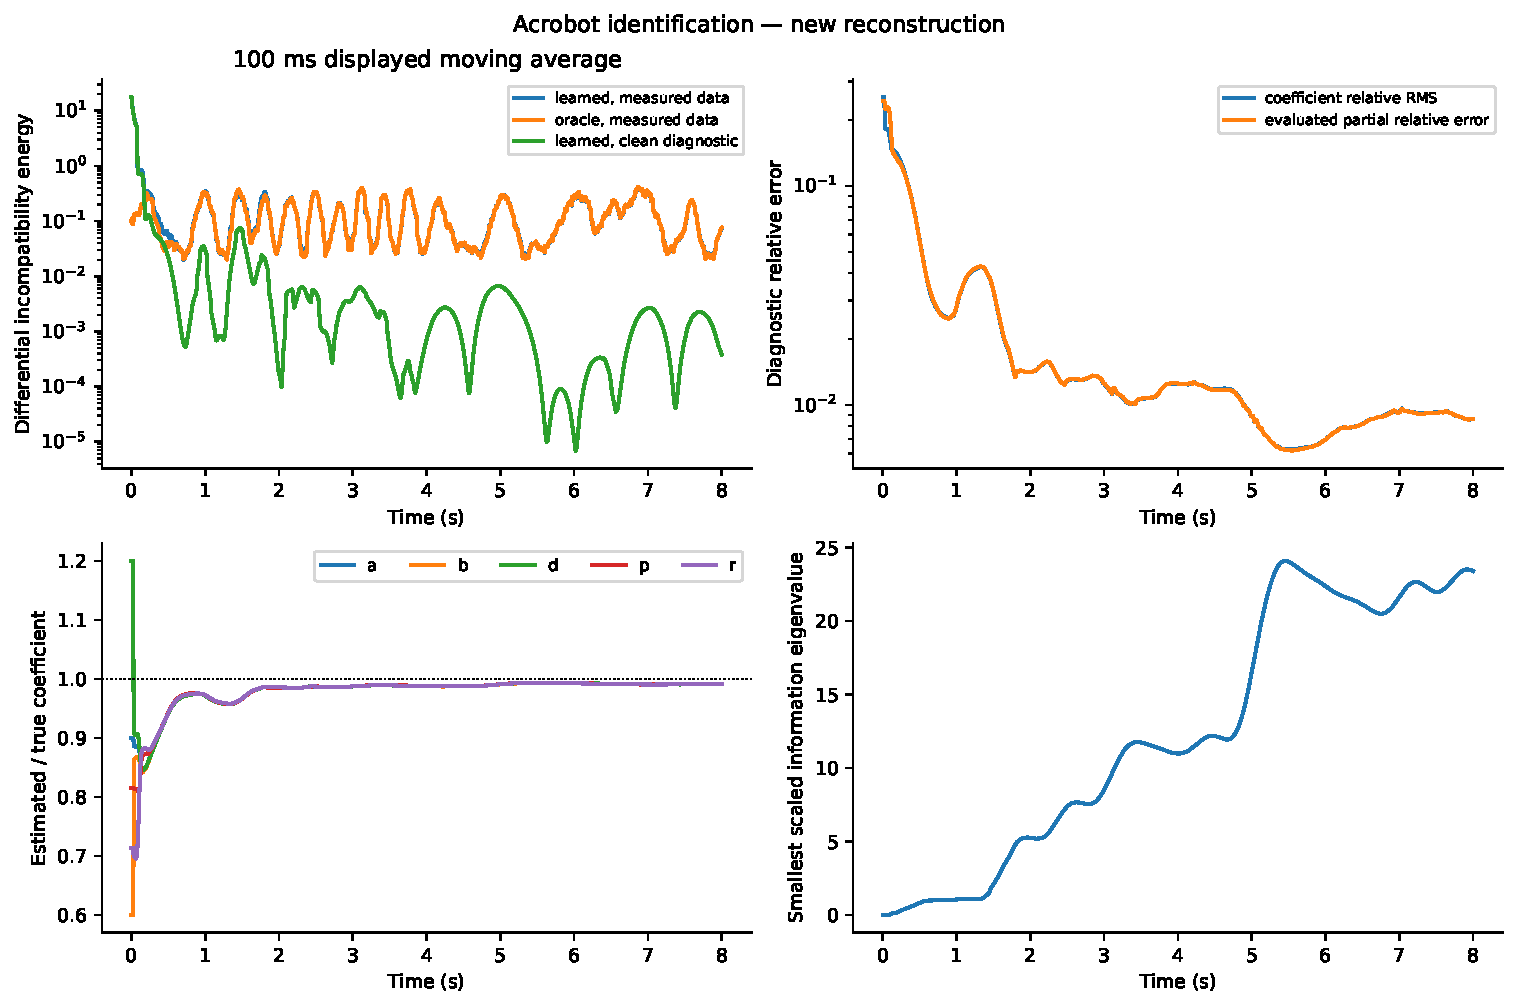
\includegraphics[width=.90\textwidth]{../examples/legacy_suite/results/acrobot/seed_10/acrobot_identification.pdf}\\[4pt]
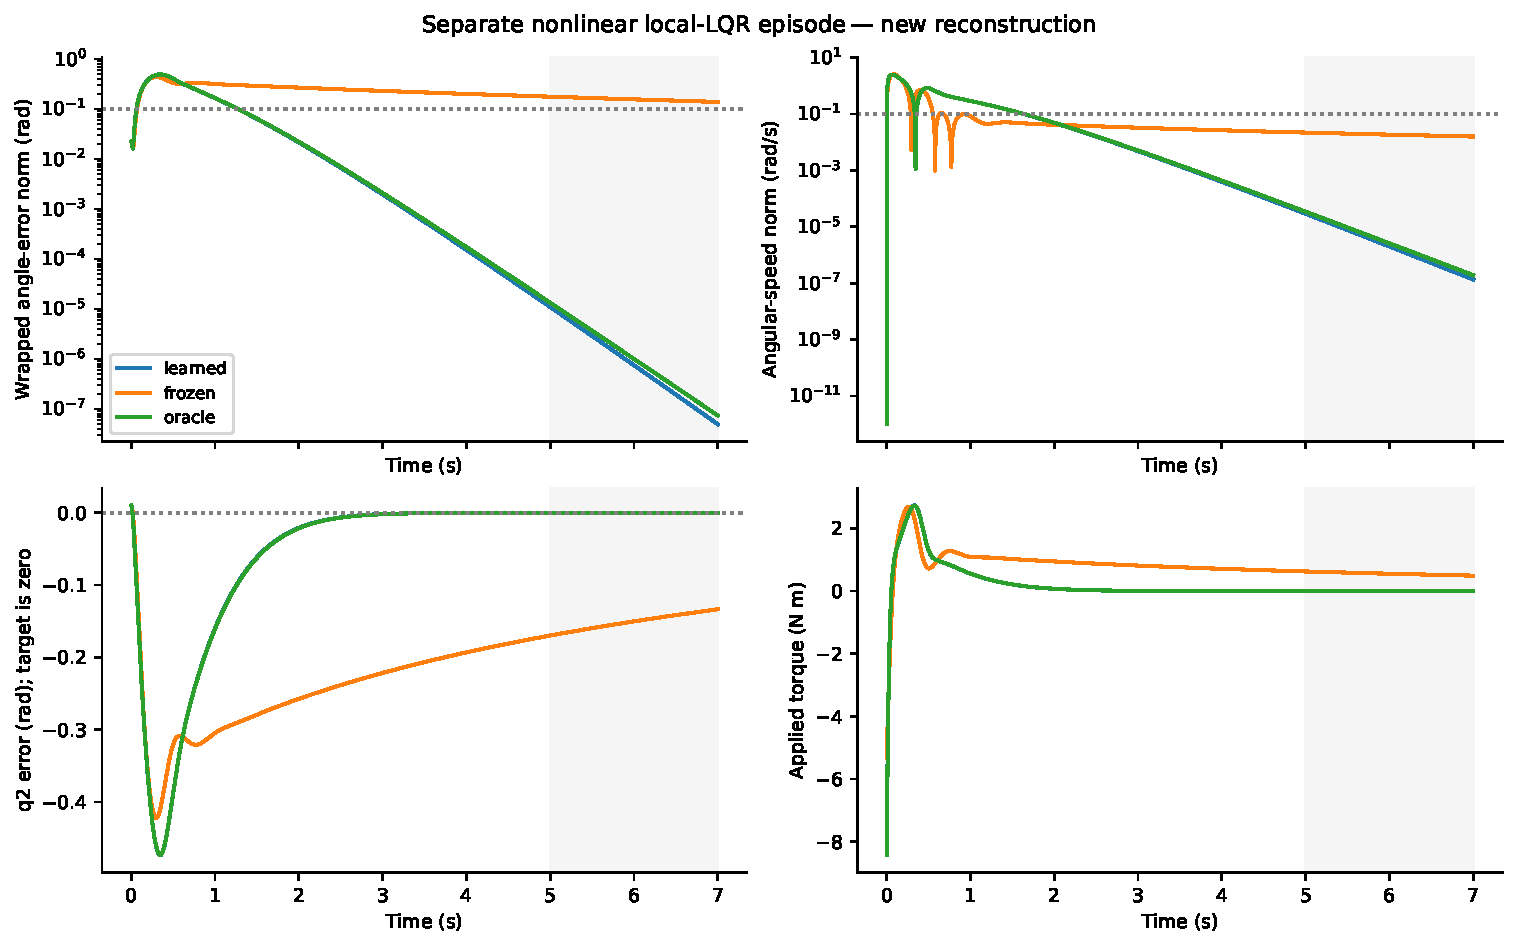
\includegraphics[width=.90\textwidth]{../examples/legacy_suite/results/acrobot/seed_10/acrobot_control.pdf}
\caption{Previously supplied Acrobot reconstruction: identification and a
separate local control episode. The source and seed-10 records are retained;
these are not newly generated ten-seed results in this revision.}
\label{fig:acrobot_archived}
\end{figure*}

\subsection{Ellipse completion: analytic illustration}
Consider $f(x,y)=x^2+2bxy+dy^2-1$ with $b=.25$ and $d=2$.
Its Jacobian is $F=(2x+2by,\,2bx+2dy)$, so compatible velocities satisfy
\begin{equation}
 (2x+2by)\dot x+(2bx+2dy)\dot y=0.
\end{equation}
Where the second coefficient is nonzero, a supplied $\dot x$ determines
$\dot y=-(x+by)\dot x/(bx+dy)$. Where the first is nonzero, the same
relation can instead compute $\dot x$ from a supplied $\dot y$.
This is an analytic illustration of query-dependent completion and its
conditioning requirement. The coefficient of $x^2$ and the residual level
are specified calibration. The historical numerical example lacks an
executable update and raw records; its figure remains an archived repository
asset but is not included or used as empirical evidence here. No numerical
learning or reproduction claim is made for this construction.

\subsection{Active flow control: an immersed-airfoil numerical prototype}
\label{sec:afc_prototype}

The previously supplied reconstruction tests structured coefficient learning and
output control on a two-dimensional
incompressible flow with an immersed NACA~0012 profile. Published surface-jet
airfoil studies motivate this setting \cite{Garcia2025Airfoil,Montala2025Wing}.
Our executable prototype uses a localized volume force and a wake-velocity
output. The geometry follows the NACA family \cite{Jacobs1933NACA}; the
numerical ingredients are obstacle penalization and incompressible projection
\cite{Angot1999Penalization,Chorin1968Projection}.

\subsubsection{Implicit system and partials}
Let $X$ be the full discrete velocity field, $A=\dot X$, and $u$ the scalar
command. With a solenoidal Fourier projection $P_h$, including the strict
two-thirds cutoff, define
\begin{align}
 N(X)&=P_h[(X\cdot\nabla_h)X],\qquad L(X)=\Delta_hX,\nonumber\\
 K(X)&=P_h[-\chi X/\eta+s(e_x-X)],\qquad B=P_hb.
 \label{eq:afc_short_operators}
\end{align}
Here $\chi$ is the smoothed body mask, $s$ is a fringe sponge, and $b$ is
the prescribed vertical body-force shape. The learned residual is
\begin{equation}
 f_\theta(X,A,u)=A+c_aN(X)-\nu L(X)-\beta Bu-K(X)=0,
 \label{eq:afc_short_f}
\end{equation}
with $\theta=(c_a,\nu,\beta)$. For $z=(X,A,u)$, its actual differential is
\begin{equation}
 F_\theta(z)=
 [\,c_aDN(X)-\nu L-DK\quad I\quad-\beta B\,].
 \label{eq:afc_short_F}
\end{equation}
The fixed rate block excludes the zero differential. Only three coefficients
of the supplied operator family are learned. The plant integrates its own
flow state; true coefficients and partials are used only for evaluation.

\subsubsection{Learning}
At observation interval $h_s$, use
$\bar X_n=(X_{n+1}+X_n)/2$ and $A_n=(X_{n+1}-X_n)/h_s$.
For $\bar z_n=(\bar X_n,A_n,u_n)$, form the causal complete-feature secant
\begin{equation}
 \xi_n^\Delta(\theta)=
 \frac{f_\theta(\bar z_n)-f_\theta(\bar z_{n-1})}{h_s},
 \label{eq:afc_short_secant}
\end{equation}
using the same candidate parameters at both endpoints. This approximates
$F_\theta(z)\dot z$ with sampling error. An exponential memory with time
constant $0.8$ minimizes the spatial mean of
$\|\xi_n^\Delta\|^2/2$, with a weak scaled quadratic regularizer and
$\theta\in[0.2,2]\times[0.0005,0.05]\times[0.15,2]$.
The three-variable box problem is solved by enumerating its active sets;
the estimate moves one quarter of the way toward the minimizer each sample.
Incompatibility is reported before updating. The imposed residual level is
checked separately on the next observed interval; it is not learned from
derivatives alone.

\subsubsection{State-dependent readout control}
Let $y=CX$ be normalized Gaussian-weighted vertical wake velocity and
$e=y-y_d$. The measured field and learned partials give
\begin{equation}
 \hat d=C[-\hat c_aN(X)+\hat\nu L(X)+K(X)],
 \qquad \hat g=\hat\beta CB.
\end{equation}
For the chosen force and readout, $CB\simeq0.128903$. The bounded regularized
readout is
\begin{align}
 u&=\operatorname{clip}_{[-2,2]}
 \frac{\hat g[\dot y_d-3e-\hat d]}{\hat g^2+10^{-4}},
 \label{eq:afc_short_control}
 \\
 y_d&=y(0)e^{-t/1.5}+0.04\sin(2\pi t/4).\nonumber
\end{align}
The reference is an output target, not an identification label.

\subsubsection{Protocol and recorded results}
The periodic domain is $6\times3$ chords, with a fringe layer, $128\times64$
grid points, nominal $Re=100$, $12^\circ$ geometric rotation, and
$\eta=0.04$. The solver uses SSP-RK3 with step $0.004$ and observes full,
noiseless fields every $0.02$. The force has opposite Gaussian lobes centered
at $(2.9,1.6)$ and $(2.9,0.65)$, of widths $(0.30,0.22)$, scaled to zero
total force. The output weight is centered at $(3.0,1.6)$ with widths
$(0.32,0.24)$. Three time units of spin-up and three of bounded multisine
identification precede six units of control. All branches start with the
same field, learned estimate, and accumulated memory. The multisine is
sampled and held at observation times; the preceding secant pair is cleared
at the control transition. At control time $2.8$, the plant actuator
gain changes from $1$ to $0.55$ without informing the learner. The
constant-coefficient compatibility identity does not apply to the
jump-crossing secant.

The actual seed-10 output RMS errors were $0.038734$ without control,
$0.004697$ with the post-identification model frozen, and $0.001216$ with
continued learning. Corresponding input RMS values were $0$, $0.675056$,
and $0.729696$, with no saturation. Final continued-learning coefficients
were $(0.998074,0.00998102,0.555842)$. Its median pre-update energy over the
final fifth of the episode was $5.12\times10^{-7}$, versus
$1.62\times10^{-4}$ for the frozen model. Very small energy in the
unactuated branch did not identify the input partial, illustrating the
need for excitation and separate partial-error diagnostics.

These are retained numerical prototype results from one seed, separate
from the main studies, the bounded Fourier comparison, and the paired
excitation study. The thin profile
is coarsely resolved, and grid, time, penalty, and domain convergence remain
unchecked. The masked-body speed is approximately $0.19$ despite divergence
RMS below $10^{-14}$. The computation establishes an executable
coefficient-learning/readout demonstration; it does not establish
direct all-entry partial learning, accurate wall
enforcement, surface-jet lift/drag improvement, or global flow stability.

\begin{figure*}[t]
\centering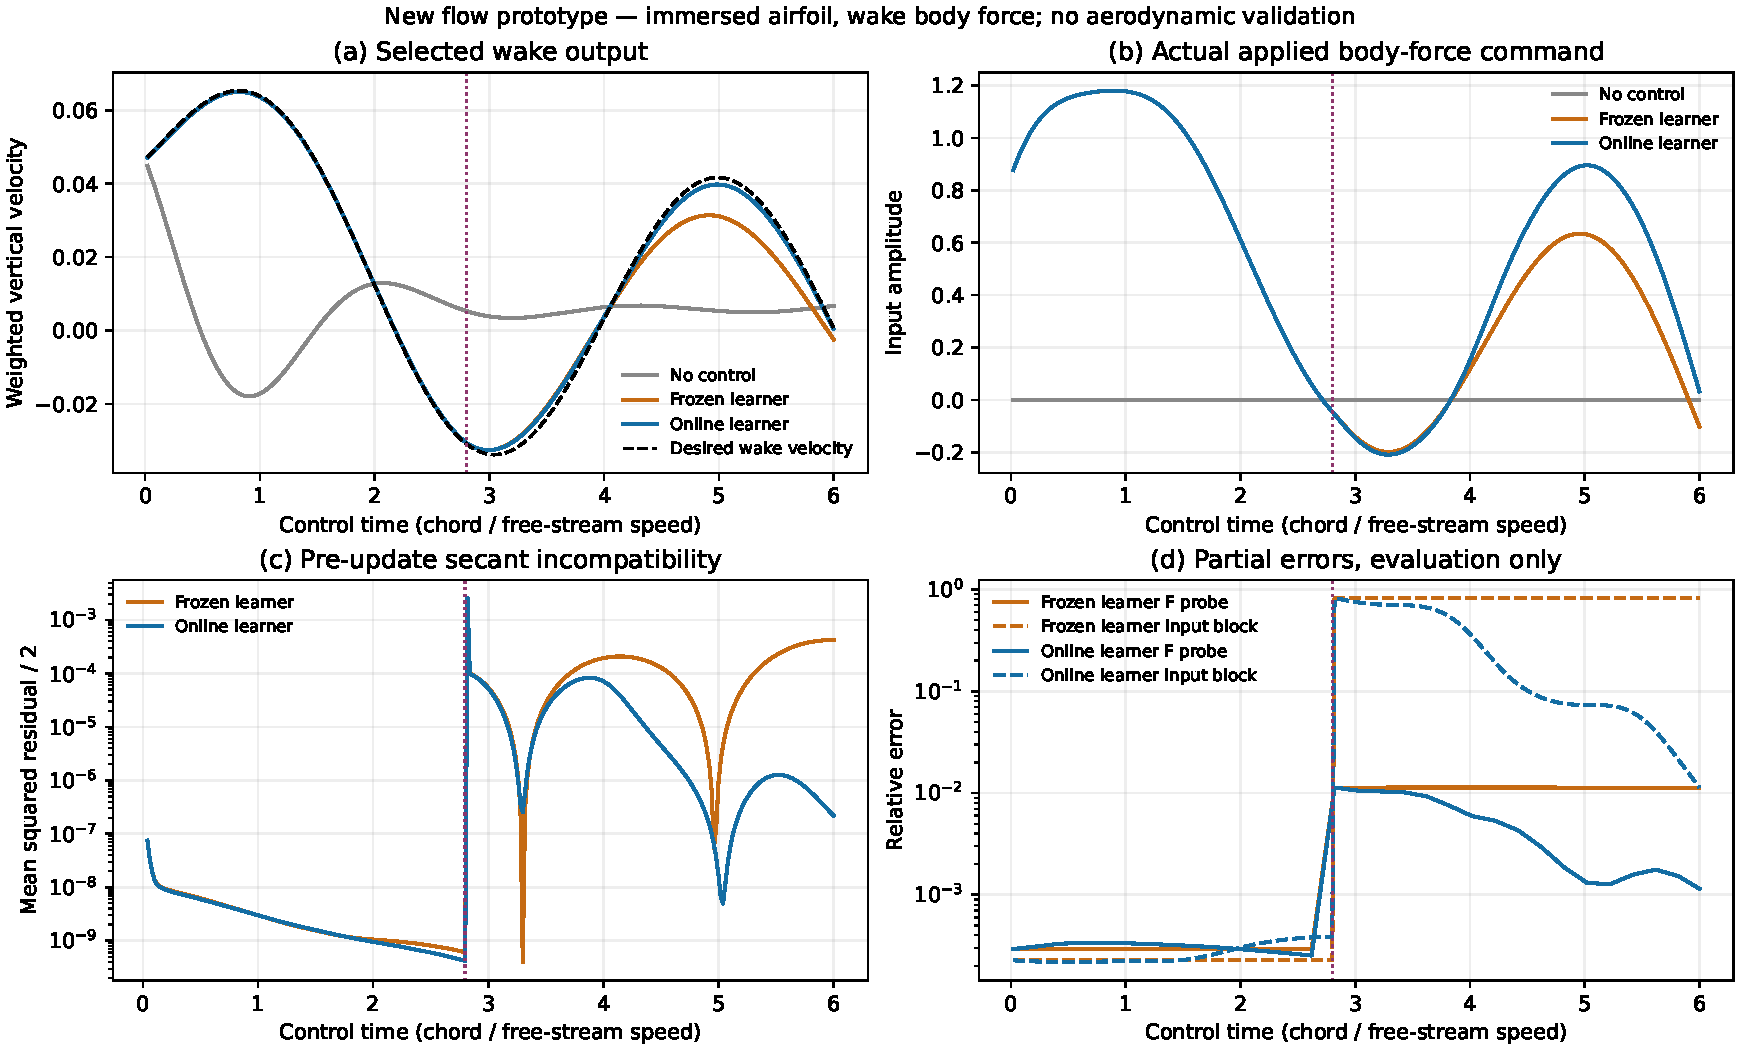
\includegraphics[width=.98\textwidth]{active_flow_results.pdf}
\caption{Previously supplied single-seed active-flow prototype results,
retained with the source and recorded data. Learning continues through an
unannounced actuator-gain change. See the explicit numerical-validation
limitations in Section~\ref{sec:afc_prototype}.}
\label{fig:flow_results}
\end{figure*}
\begin{figure*}[t]
\centering
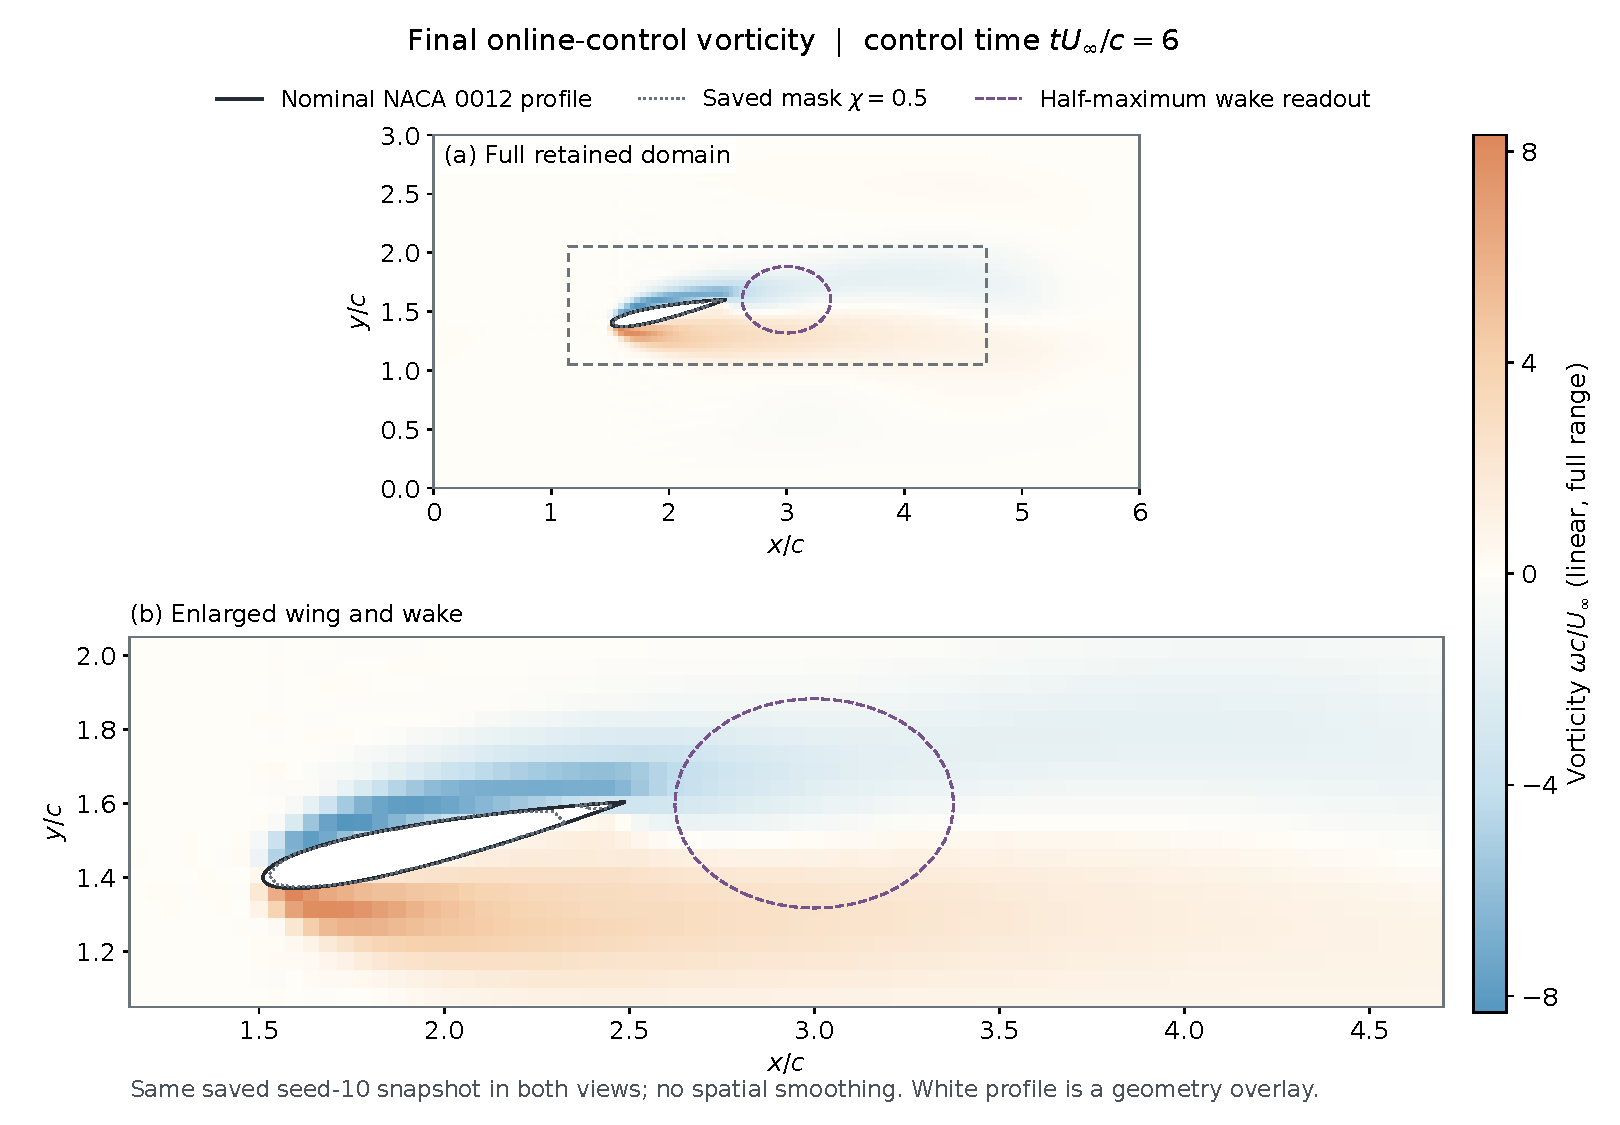
\includegraphics[width=.98\textwidth]{active_flow_vorticity.pdf}\\[5pt]
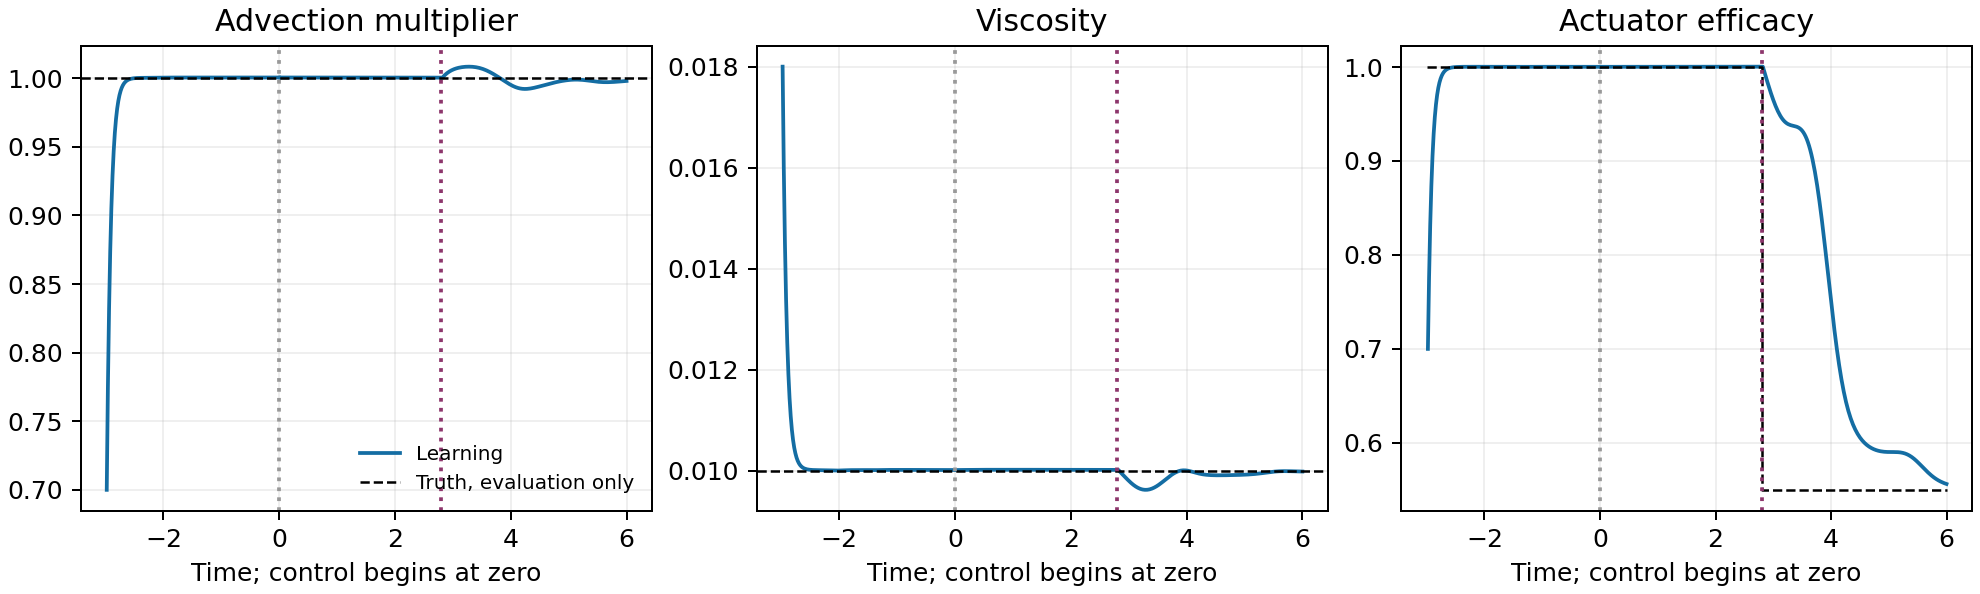
\includegraphics[width=.94\textwidth]{active_flow_parameters.png}
\caption{Retained seed-10 flow prototype: final online-control vorticity
at control time $tU_\infty/c=6$, followed by the original coefficient
trajectories. The full-domain and enlarged wing/wake views use the same saved
velocity field, its spectral curl, and a shared linear color scale spanning
the full vorticity range (no percentile clipping or spatial smoothing).
The white shape is the nominal NACA~0012 profile; the dotted contour is the
saved immersed mask $\chi=0.5$, and the purple dashed contour marks the
half-maximum wake readout weight. The coarse mask differs from the nominal
profile. These are legacy structured-coefficient results, not a demonstration
of unrestricted direct-partial learning or validated aerodynamic performance.}
\label{fig:flow_fields}
\end{figure*}
\begin{figure*}[t]
\centering
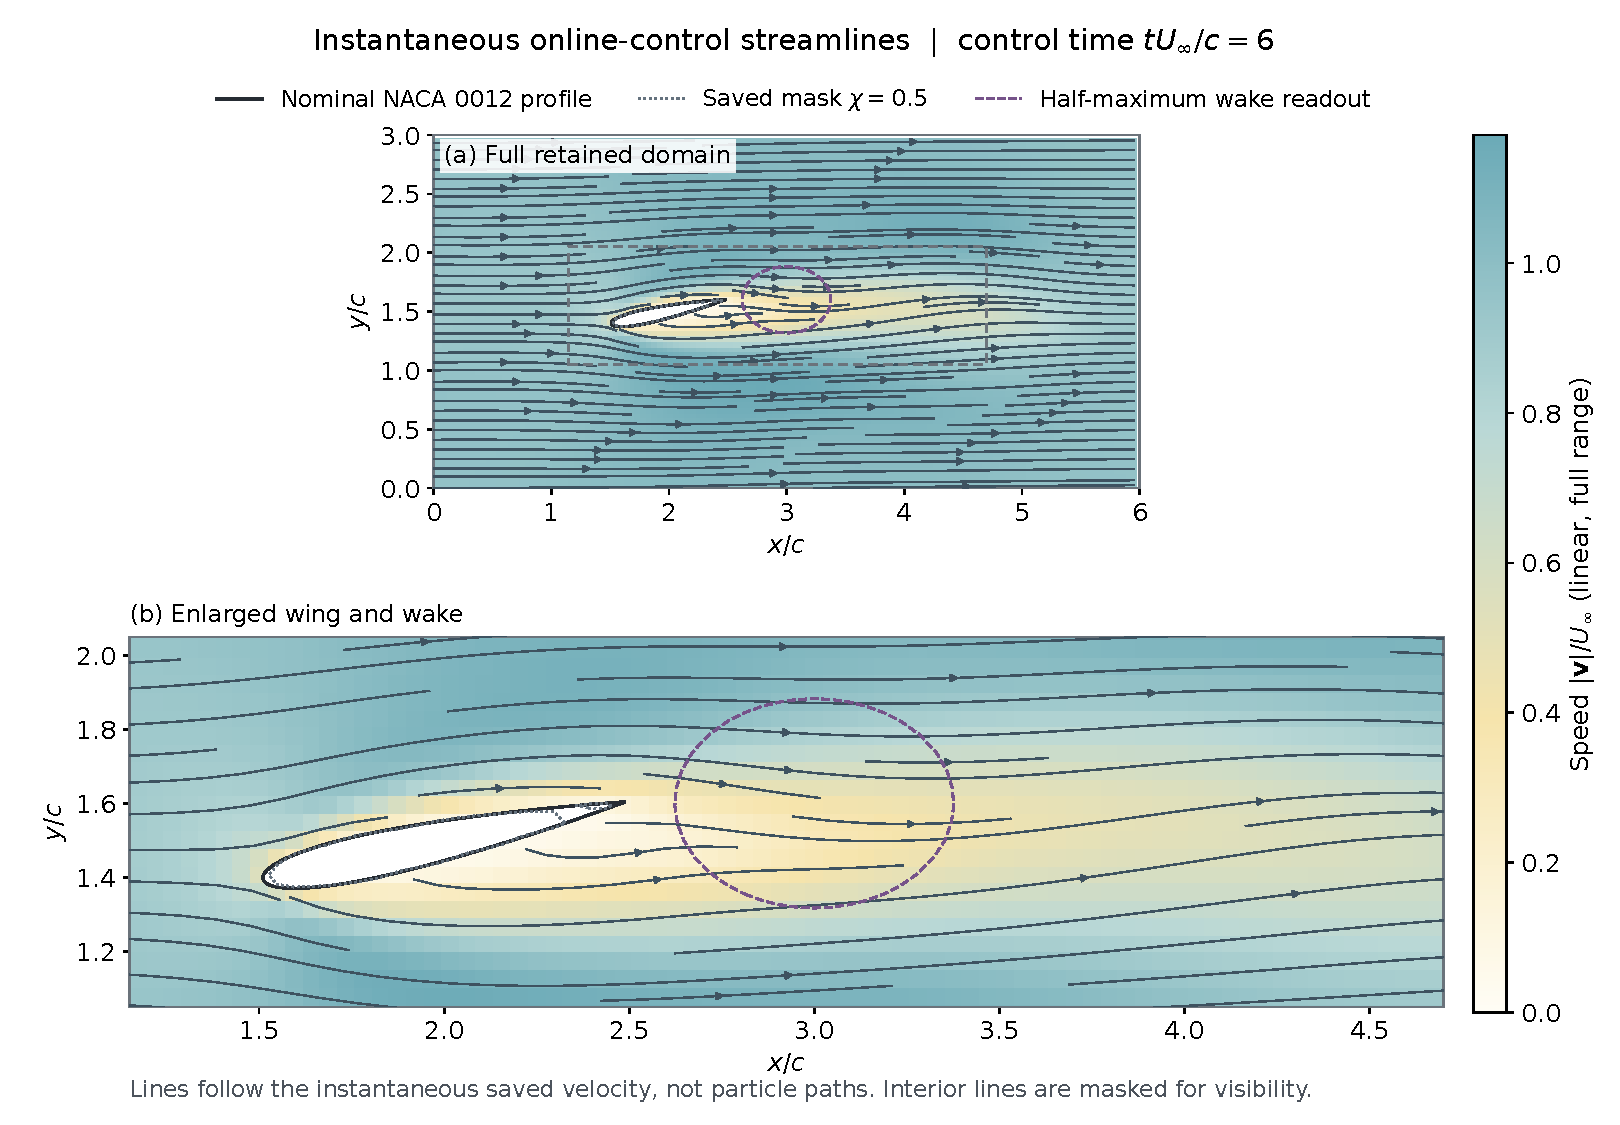
\includegraphics[width=.98\textwidth]{active_flow_streamlines.pdf}
\caption{Instantaneous streamlines of the same saved online-control velocity
field as Fig.~\ref{fig:flow_fields}, at control time $tU_\infty/c=6$.
Arrows indicate flow direction; the background shows speed on a shared,
full-range linear scale. Lines use bilinear interpolation of the recorded
velocity and are instantaneous streamlines, not particle trajectories.
For visibility, lines are masked inside the nominal profile or where
$\chi\geq0.5$; the white geometry overlay hides the body interior. This display
mask does not establish no penetration: the retained immersed-body speed
RMS is approximately $0.19$, and boundary, grid, and time convergence remain
unvalidated. Geometry and readout contours follow Fig.~\ref{fig:flow_fields}.}
\label{fig:flow_streamlines}
\end{figure*}

\section{Verification and interpretation limits}
Finite-difference tests check the contact differential and the Fourier clock
column. Tests check projected energy descent, current-candidate memory,
pre-update scoring, gauge invariance, fixed coefficients in frozen branches,
and numerical consistency. The prior 27-test suite is retained and executed
separately. Independent postprocessing recomputes the retained structured-study metrics
from saved traces; current direct-study checks are in
Section~\ref{sec:direct_main}. These checks establish computational consistency, not physical
validation or a global closed-loop guarantee.

The original structured-study plots use causal moving averages only for
energy: 1 s in contact and bounded Fourier, and .25 s in Burgers. Other curves are unsmoothed (some are displayed
at a fixed decimation for legibility). All unaveraged values remain in the
traces. Logarithmic display floors affect rendering only, never reported
metrics. The fixed physical families determine gauge and level; they do not
establish unrestricted differential discovery. The separate retained anchor-free
example addresses normalization without a privileged derivative block.
Section~\ref{sec:unanchored} includes its checked reconstructed figure and
executable records. The historical figure with unresolved lineage is no
longer included. The direct-learning and normalized-plant experiments below
are separately identified and fully recorded, with their display aggregation
specified in the corresponding captions.

\clearpage
% Supporting analysis of the public implementations. No main-paper proof is
% moved here, and this file has no dependency on the private manuscript.
\newtheorem{auditproposition}{Proposition}
\renewcommand{\theauditproposition}{S.A\arabic{auditproposition}}

\section{Learning-rule audit and additional supporting proofs}
\label{sec:learning_rule_audit}

This section audits the retained coefficient-based contact, Burgers, and
bounded Fourier studies; the current direct-field main experiments are
documented separately in Section~\ref{sec:direct_main}.
They estimate coefficients of prescribed implicit relations
and obtain their evaluated context partials by differentiation. Their adaptive
updates receive observed features, not target Jacobian entries. This is
coefficient estimation with a structured differential evaluation. It is
not the direct all-entry learning mechanism specified in
Section~\ref{sec:scope}: physical
coefficients, feature families, residual levels, and selected sensing channels
are supplied. These studies implement constrained sampled
coefficient updates; they do not numerically integrate the unrestricted
row-Stiefel learning flow. The distinctions below specify what the numerical
evidence can support. The retained normalized Fourier experiment is audited
separately in Section~\ref{sec:normalized_fourier_results}; it adapts all
seven coefficients and numerically integrates the coupled normalized law,
but still derives its partials from a supplied residual family.

\subsection{Exact update, scaling, and current-candidate memory}
Write the physical free coefficients as $c=D_s\theta$, where $D_s$ is the
positive diagonal matrix of optimization scales. For observed free features
$a_{n,\ell}$ and a supplied contribution $b_{n,\ell}$, the implemented
implicit feature row is
\begin{equation}
 v_{n,\ell}=\col(D_sa_{n,\ell},b_{n,\ell}),\qquad
 q_\theta=\col(\theta,1).
 \label{eq:audit_channels}
\end{equation}
Thus $q_\theta^{\mathsf T}v_{n,\ell}=c^{\mathsf T}a_{n,\ell}+b_{n,\ell}$;
scaling changes optimization coordinates, not the physical residual.
Let $N_n$ be the number of simultaneous spatial samples and let
$\beta=\exp(-h/\tau_m)$. After scoring the new sample with $\theta_{n-1}$,
the code sets
\begin{align}
 R_n&=\beta R_{n-1}+\frac{1-\beta}{N_n}
       \sum_{\ell=1}^{N_n}v_{n,\ell}v_{n,\ell}^{\mathsf T},\\
 H_n&=(R_n)_{1:p,1:p},\qquad g_n=(R_n)_{1:p,p+1}.
\end{align}
Starting from $R_0=0$ and $\theta_n^{(0)}=\theta_{n-1}$, it sets
\begin{align}
 \alpha_n&=\frac{1}{\max(\tr H_n,10^{-12})},\\
 \theta_n^{(j+1)}&=\Pi_{\mathcal W}
 \bigl(\theta_n^{(j)}-\alpha_n(H_n\theta_n^{(j)}+g_n)\bigr).
 \label{eq:audit_exact_update}
\end{align}
The output is $\theta_n=\theta_n^{(M)}$ and $\mathcal W$ is the scaled
coefficient box. Contact uses $M=48$;
Bounded Fourier and Burgers use $M=8$. Burgers stores its unscaled moment with
the fixed channel first; permuting that channel and applying $D_s$ gives
exactly the same recurrence. Material and secant observations begin only
when the specified observation window is full. Contact's kinematic rows
start accumulating at the first sample. At the terminal sample the memory
may still be updated, but the coefficients and physical state are not.

\begin{auditproposition}[One candidate over the entire stored history]
\label{prop:audit_memory}
For any sequence of observed feature rows and any candidate $\vartheta$,
including a candidate never used when the data were collected,
\begin{equation}
 \frac12q_\vartheta^{\mathsf T}R_nq_\vartheta
 =\frac{1-\beta}{2}\sum_{i=1}^{n}\frac{\beta^{n-i}}{N_i}
   \sum_{\ell=1}^{N_i}(q_\vartheta^{\mathsf T}v_{i,\ell})^2.
 \label{eq:audit_memory_identity}
\end{equation}
Its free gradient is $H_n\vartheta+g_n$. Each inner step in
(\ref{eq:audit_exact_update}) decreases this fixed objective by at least
$\|\theta_n^{(j+1)}-\theta_n^{(j)}\|^2/(2\alpha_n)$.
\end{auditproposition}
\begin{IEEEproof}
Unrolling the linear recursion gives
$R_n=(1-\beta)\sum_{i=1}^n\beta^{n-i}N_i^{-1}
\sum_\ell v_{i,\ell}v_{i,\ell}^{\mathsf T}$.
Multiplication by the same $q_\vartheta$ on both sides proves
(\ref{eq:audit_memory_identity}); differentiation gives the stated
gradient. Let $d=\theta^+-\theta$ for one projected step. Projection onto
the convex box gives $(H_n\theta+g_n)^{\mathsf T}d\le-\|d\|^2/\alpha_n$.
The exact quadratic expansion then gives
\begin{align*}
 \mathcal J_n(\theta+d)-\mathcal J_n(\theta)
 &\le-\|d\|^2/\alpha_n+d^{\mathsf T}H_nd/2\\
 &\le-\|d\|^2/(2\alpha_n),
\end{align*}
because $H_n\succeq0$ and
$\alpha_n\lambda_{\max}(H_n)\le\alpha_n\tr H_n\le1$.
\end{IEEEproof}
The identity holds for dependent, overlapping, closed-loop observations;
independence is unnecessary for this algebra. It proves that old residuals
are reevaluated at the current candidate through sufficient statistics.
It does not prove statistical consistency, physical excitation, or monotone
energy when a new observation changes $R_n$.

\subsection{What is observed and what is learned}
\subsubsection{Contact}
The material relation is
\begin{equation}
 f_c=\dot\lambda-s^{\mathsf T}\beta(x)+ay+\rho\lambda
       -r^{\mathsf T}\beta'(x)v_x+bv_y=0,
 \label{eq:audit_contact_relation}
\end{equation}
with learned $c=\col(s,a,r,b)$. Its partials, in the declared context
$(x,y,\lambda,v_x,v_y,\dot\lambda,u_1,u_2)$, are
\begin{equation}
 F_c=\bigl[-s^{\mathsf T}\beta'(x)-r^{\mathsf T}\beta''(x)v_x,
 a,\rho,-r^{\mathsf T}\beta'(x),b,1,0,0\bigr].
 \label{eq:audit_contact_partials}
\end{equation}
The two additional rows come from $v-Bu=0$; their velocity identity block
is supplied and their input block $-B$ is learned. Both material vectors
$s,r$, both material scalars $a,b$, and all four entries of $B$ adapt.
The constant $\rho=4$, the unit coefficient of $\dot\lambda$, the unit
velocity block, and the functional form of $\beta$ are supplied.

Let $\Delta$ be the material observation window and let $\delta$ denote
its endpoint difference. Integrating (\ref{eq:audit_contact_relation})
with one fixed candidate gives the observed material incompatibility
\begin{equation}
 \begin{split}
 \xi_c=\Delta^{-1}\biggl[&\delta\lambda-s^{\mathsf T}\!\int\beta(x)\dd t
 +a\!\int y\dd t\\
 &+\rho\!\int\lambda\dd t-r^{\mathsf T}\delta\beta(x)+b\delta y\biggr].
 \end{split}
 \label{eq:audit_contact_integral}
\end{equation}
The implementation uses trapezoidal quadrature and measured force for
$\lambda$; it does not train on clean $\dot\lambda$ or on a target $F_c$.
The kinematic learner uses the instantaneous measured residual $v_m-Bu$.
Consequently these two contact updates use calibrated integral-level and
velocity-level relations, respectively. They are not measurements of the
raw-context differential incompatibility $F\dot z$. At the material
change, a window can contain two different physical coefficient sets;
such windows are retained and marked, rather than assumed exactly
compatible with either fixed coefficient vector.

The controller estimates the surface slope from the noisy two-component
force measurement:
\begin{equation*}
 \widehat h'_m=-f_{m,x}/\max(f_{m,y},0.2).
\end{equation*}
The simulator generates
that force through the true surface, as a physical sensor would respond to
the environment. The controller does not receive the true geometric
coefficient vector. Its curvature estimate uses the learned ratio $s/a$.
Thus geometry is partly observed through force direction and partly
inferred through the learned relation. The true surface also fixes the
initial physical contact and the evaluator's indentation diagnostic.
These are separate from the adaptive update.

\subsubsection{Bounded Fourier comparison}
For $h(\phi)=(1,\cos\phi,\sin\phi)^{\mathsf T}$,
the learned six coefficients define
\begin{align}
 \rho_c(\phi)&=c_\rho^{\mathsf T}h(\phi),&
 \kappa_c(\phi)&=c_\kappa^{\mathsf T}h(\phi),\\
 f_c(x,v,u,\phi)&=\rho_c(\phi)v+\kappa_c(\phi)x-u.
\end{align}
The evaluated derivative is
\begin{equation}
 F_c=\bigl[\kappa_c,\rho_c,-1,
 c_\rho^{\mathsf T}h'(\phi)v+c_\kappa^{\mathsf T}h'(\phi)x\bigr].
 \label{eq:audit_fourier_partials}
\end{equation}
The state, rate, and phase columns therefore depend on learned coefficients;
only the input partial $-1$ is fixed. The rate measurement is noisy; the
state and phase are exact in this model. The phase law $\phi=4t$ and the
harmonic basis are supplied, so the experiment does not learn a frequency
or discover the basis. The displayed phase partial is with respect to
$\phi$, not $t$; the clock contribution along the trajectory is multiplied
by $\dot\phi=4$.

The learner differences the complete observed feature vector
$(h(\phi)v_m,h(\phi)x,-u)$ over the declared window, with the same current
coefficient vector at both endpoints. Thus the phase-state and phase-rate
product terms are retained. A $K=0$ shadow receives the identical stream
but is restricted to two constant coefficients; it has the same memory
mechanism. It is a basis ablation, not an independent estimator of matched
capacity. The separate $K=0$ controller generates its own trajectory.

\subsubsection{Burgers}
At each grid point, with context $(w,w_s,w_{ss},u,w_t)$,
\begin{align}
 f_c&=w_t+c_a w w_s-\nu w_{ss}-bu,\\
 F_c&=(c_a w_s,c_a w,-\nu,-b,1).
 \label{eq:audit_burgers_partials}
\end{align}
The three coefficients $c_a,\nu,b$ adapt. Four of the five evaluated
partials depend on those coefficients; the $w_t$ partial is supplied.
The learner differences complete features $(w_{t,m},ww_s,-w_{ss},-u)$,
including the nonlinear product as a whole. State values and their
spectral spatial derivatives are exact sensing channels; only $w_t$ is
noisy. The plant and learner use the same collocation product and spatial
operators, with full-field sensing and actuation. This is a matched
semidiscrete-model experiment, not independent continuous-PDE validation
or evidence for sparse sensors, unknown spatial operators, or model mismatch.

\subsection{Complete-feature secants and the derivative being estimated}
\begin{auditproposition}[Fixed-candidate secant identity]
\label{prop:audit_secant}
Let $f_\theta(z)=Q_\theta\zeta(z)$ be continuously differentiable on the
line segment between $z_-$ and $z_+$ and fix $\theta$. For $\Delta>0$,
\begin{align}
 Q_\theta\frac{\zeta(z_+)-\zeta(z_-)}{\Delta}
 &=\frac{f_\theta(z_+)-f_\theta(z_-)}{\Delta}\\
 &=\frac{1}{\Delta}\int_0^1 F_\theta(z_-+s\delta z)\delta z\dd s,
 \label{eq:audit_secant_identity}
\end{align}
where $\delta z=z_+-z_-$. If $F_\theta$ is $K$-Lipschitz on that segment,
the difference between this secant and
$F_\theta(z_-)\delta z/\Delta$ is at most
$K\|\delta z\|^2/(2\Delta)$.
\end{auditproposition}
\begin{IEEEproof}
Linearity gives the first equality. Apply the fundamental theorem of
calculus to $s\mapsto f_\theta(z_-+s\delta z)$ for the second. Subtract
$F_\theta(z_-)\delta z/\Delta$ inside the integral and use
$\|F_\theta(z_-+s\delta z)-F_\theta(z_-)\|\le Ks\|\delta z\|$;
integration of $s$ over $[0,1]$ gives the bound.
\end{IEEEproof}
This result includes every complete-product and clock term without
assuming that held commands are temporally smooth. The segment is an
algebraic interpolation of context endpoints, not a claim that the plant
followed that segment. With noisy endpoints or command changes, the
observed secant is not an exact instantaneous sample of $F\dot z$.

In all three models $F_\theta=D_zf_\theta$ holds with the candidate fixed.
If both the state and coefficients vary, the different identity
\begin{equation}
 \frac{\dd}{\dd t}f_{\theta(t)}(z(t))
 =F_{\theta(t)}(z(t))\dot z(t)
   +\partial_\theta f_{\theta(t)}(z(t))\dot\theta(t)
 \label{eq:audit_adapting_residual}
\end{equation}
contains the parameter term. The code does not difference residual values
evaluated with old coefficients at one endpoint and new coefficients at
the other, so it does not inadvertently insert or omit this adaptation
term in a fixed-candidate derivative. Compatibility alone also cannot
identify an additive residual level: $f$ and $f+C$ have the same
differential and complete-feature differences. The direct readouts use
the explicitly supplied zero level.

\subsection{A conditional tracking bound for the actual sampled update}
The following result applies to the implemented box-constrained quadratic
update. It makes no identification claim when excitation is absent and
does not import a Stiefel-flow convergence rate.

\begin{auditproposition}[Optimization tracking and physical bias]
\label{prop:audit_tracking}
At each observation $n$, suppose $\mathcal W$ is a fixed nonempty closed
convex set, $\mu_n I\preceq H_n\preceq L_nI$ with $\mu_n>0$, and
$0<\alpha_n\le1/L_n$. Let $\theta_n^\circ$ be the unique minimizer
of $\mathcal J_n$ over $\mathcal W$, and let $M_n\ge1$ projected steps begin
at $\theta_{n-1}$. Define
\begin{equation}
 r_n=(1-\alpha_n\mu_n)^{M_n},\quad
 d_n=\|\theta_n^\circ-\theta_{n-1}^\circ\|,\quad
 e_n=\|\theta_n-\theta_n^\circ\|.
\end{equation}
Then $e_n\le r_n(e_{n-1}+d_n)$. If $r_n\le\bar r<1$ and
$d_n\le\bar d$ on an interval of $n$ observations,
\begin{equation}
 e_n\le\bar r^{\,n}e_0+
       \frac{\bar r(1-\bar r^{\,n})}{1-\bar r}\bar d.
 \label{eq:audit_optimizer_tracking}
\end{equation}
For any feasible physical coefficient target $\theta_n^*$,
\begin{equation}
 \|\theta_n^\circ-\theta_n^*\|
 \le\frac{\|\nabla\mathcal J_n(\theta_n^*)\|}{\mu_n}.
 \label{eq:audit_physical_bias}
\end{equation}
The indices can be restarted after a warm-up interval on which positive
curvature was not available.
\end{auditproposition}
\begin{IEEEproof}
The minimizer satisfies the projection fixed-point identity
$\theta_n^\circ=\Pi_{\mathcal W}(\theta_n^\circ-
\alpha_n\nabla\mathcal J_n(\theta_n^\circ))$.
Projection is nonexpansive, while the difference of the two unprojected
updates is $(I-\alpha_nH_n)(\theta-\theta_n^\circ)$.
The eigenvalues of this symmetric matrix lie in
$[0,1-\alpha_n\mu_n]$, proving contraction by that factor. Iterating
$M_n$ times and applying the triangle inequality to the previous target
gives $e_n\le r_n(e_{n-1}+d_n)$. Unrolling this scalar recurrence
gives (\ref{eq:audit_optimizer_tracking}).

For the bias claim set $d=\theta_n^\circ-\theta_n^*$.
The variational inequality at the constrained minimizer gives
$d^{\mathsf T}\nabla\mathcal J_n(\theta_n^\circ)\le0$.
Since the gradient difference is $H_nd$,
\begin{equation*}
 \mu_n\|d\|^2\le d^{\mathsf T}H_nd
 \le-d^{\mathsf T}\nabla\mathcal J_n(\theta_n^*)
 \le\|d\|\,\|\nabla\mathcal J_n(\theta_n^*)\|.
\end{equation*}
Divide by $\|d\|$ when nonzero; the zero case is immediate.
\end{IEEEproof}
Here $\nabla\mathcal J_n(\theta_n^*)$ measures retained-data
incompatibility in free-coefficient directions. It can be nonzero because
of sensing noise, quadrature, model mismatch, or a physical change within
retained history. A positive empirical curvature caused partly by noise
does not imply a small bias term. At a material jump the target drift can
be large; neither the bound nor the experiment implies instantaneous
tracking. When $H_n$ is singular, the descent result remains valid but
strict contraction and unique identification do not follow.

\subsection{From coefficient error to evaluated derivative error}
For any of these prescribed families, stack its evaluated partials into
one vector and write
\begin{equation}
 \operatorname{vec}F_\theta(z)=a(z)+B(z)\theta.
 \label{eq:audit_partial_map}
\end{equation}
The fixed terms are in $a$; optimization scales are included in $B$.
Equations (\ref{eq:audit_contact_partials}),
(\ref{eq:audit_fourier_partials}), and
(\ref{eq:audit_burgers_partials}) specify this map directly.

\begin{auditproposition}[Evaluated derivative tracking]
\label{prop:audit_partial_error}
Let $W$ be any fixed diagonal weighting of vectorized partial entries and
let $P_U$ be the diagonal coordinate mask, of the same dimension,
that retains only entries depending on unknown coefficients.
At a common context $z$, the same-family coefficient target obeys
\begin{align}
 \|WP_U\operatorname{vec}(F_\theta-F_{\theta^*})\|
 &\le\|WP_UB(z)\|\,\|\theta-\theta^*\|.\label{eq:audit_partial_error}
\end{align}
Under Proposition~\ref{prop:audit_tracking}, this error for $\theta_n$
is bounded by
\begin{equation}
 \|WP_UB(z)\|
 \left(e_n+\frac{\|\nabla\mathcal J_n(\theta_n^*)\|}{\mu_n}\right).
 \label{eq:audit_partial_tracking}
\end{equation}
If the physical differential is not in the family, its discrepancy from
$F_{\theta_n^*}$ must be added to the right-hand side.
\end{auditproposition}
\begin{IEEEproof}
Subtract (\ref{eq:audit_partial_map}) at $\theta$ and $\theta^*$.
The fixed part cancels and the operator-norm inequality gives
(\ref{eq:audit_partial_error}). Use the triangle inequality
$\|\theta_n-\theta_n^*\|\le e_n+
\|\theta_n^\circ-\theta_n^*\|$ and
(\ref{eq:audit_physical_bias}) for the second conclusion. A second
triangle inequality adds any outside-family discrepancy.
\end{IEEEproof}
This calculation explains both the capability and its limitation:
constant learned coefficients can represent rapidly changing evaluated
partials, but successful optimization does not ensure accurate physical
partials without small bias and a suitable family. The norm of $B(z)$
can amplify coefficient error, especially in the Fourier phase column
or contact curvature term. This is why evaluated partials, rather than
coefficient error alone, are reported.
The reported pre-update partials use $\theta_{n-1}$ at the current context.
For those scores, the same bound holds with $e_n$ replaced by
$e_{n-1}+d_n$; this follows before applying the current optimization
steps. Post-update improvement is not substituted for pre-update accuracy.
For contact, the optimizer bound is applied separately to the material
fit and each kinematic row, using their own curvature and step sizes;
the three coefficient-error bounds combine by the Euclidean norm before
applying the full derivative map. A common step size across these fits
is not assumed.

The unknown-only diagnostic excludes the supplied $\rho$, unit blocks,
and fixed zero entries in contact; the $-1$ input partial in Fourier;
and the unit $w_t$ partial in Burgers. With the same physical scaling,
define
\begin{equation}
 e_{F,U}=\frac{\|WP_U\operatorname{vec}(\widehat F-F)\|}
 {\|WP_U\operatorname{vec}F\|}.
 \label{eq:audit_unknown_only}
\end{equation}
This ratio requires a nonzero denominator; zero-denominator cases must
be reported separately. Correct supplied blocks contribute nothing to
the error numerator but increase the full-matrix denominator, so full
relative errors can understate error in learned entries. Both conventions
should be distinguished. Neither pointwise derivative accuracy nor a
small compatibility energy alone establishes closed-loop stability.

\subsection{Information-flow checks and remaining limitations}
The public test file \path{tests/test_information_boundaries.py}
deliberately replaces the clean diagnostic histories and the evaluated
Jacobian functions with corrupted values while preserving the plant,
sensors, references, and random stream. For the three structured learned branches,
the physical trajectories, controls, and learned coefficient sequences
remain identical; the diagnostic outputs change. A positive-control test
changes Fourier's measured rate noise and observes changed learning,
while preserving the first premeasurement command. Another test forbids
access to the true-coefficient configuration when constructing and
updating the Burgers learner. These tests complement source tracing and
the existing finite-difference and current-candidate memory tests. They
do not constitute a proof that every possible future code change or
unexamined branch is free from information leakage.

The present audit found no evaluator-to-learner or evaluator-to-controller
path in the adaptive branches examined. True coefficients generate the
physical plant and simulated measurements, and are used by explicitly
named oracle baselines and evaluators. This is different from supplying
them as learning targets. Nevertheless, the examples assume correct
functional families, physically informed coefficient boxes, selected
known coefficients, and calibrated levels. Fourier additionally supplies
phase and frequency; Burgers supplies exact state/spatial channels and
matched discretization; contact measures force direction. These declared
advantages prevent interpreting the experiments as unrestricted equation
discovery or as validation of every convergence hypothesis of the
continuous-time theory.

% New, separately identified supplementary experiment. Generated figures/tables
% are public assets; full raw records are kept outside this repository.
\newtheorem{directproposition}{Proposition}
\renewcommand{\thedirectproposition}{S.D\arabic{directproposition}}

\section{Direct lifted rate-field learning and recovery after a change}
\label{sec:direct_lift_results}
The retained coefficient-based contact, Burgers, and bounded Fourier studies
supply some derivative blocks and infer the remaining entries through physical
coefficients. This additional historical experiment
tests the normalized learning rule directly in a lifted rate family, with
all six coefficient entries adaptive and no fixed derivative entry.
It is a separately identified supplementary protocol,
\texttt{direct\_lift\_20261118\_v1}; it neither replaces the current direct
main experiments in Section~\ref{sec:direct_main} nor recovers missing
historical records. There is no controller,
command readout, or claimed closed-loop stability result in this benchmark.
Its known-phase kinematic stream also supplies no independently varied
physical input against which faster partial variation is established.
It is a retained field-learning diagnostic, not the requested complete
Fourier Memory application now documented in Section~\ref{sec:direct_main}.

\subsection{Observation model, target, and independent protocol}
The context is $z=(x,y)$ with $x=t$, and the measured tangent is
\begin{equation}
 v_m(t)=\begin{bmatrix}1\\-A(t)\cos t+\varepsilon(t)\end{bmatrix},
 \qquad \varepsilon_n\sim\mathcal N(0,0.005^2).
 \label{eq:direct_observations}
\end{equation}
The first coordinate and phase are exact clock channels. Only the second
rate is noisy. The kinematic stream is generated directly, rather than
by a separately discretized physical plant. The stationary scenario has
$A=1$ throughout; the change scenario has $A=1$ before 60~s and $A=1.6$
thereafter. Both run from 0 to 120~s with $h=0.02$~s, exponential memory
$\tau_m=8$~s, gain $\eta=10$, and seeds 10--19. All twenty specified
runs are retained. Random sensor noise is the only between-seed variation;
the two scenarios share their pre-change stream for the same seed.

The clean target row is $F_*(x)=(A\cos x,1)$ within each stationary
segment. For a constant $A$, it is the Jacobian of $y+A\sin x$. For the
change at $x_c=60$, define
\begin{equation}
 g(x)=\begin{cases}
 A_1\sin x,&x<x_c,\\
 A_1\sin x_c+A_2(\sin x-\sin x_c),&x\ge x_c.
 \end{cases}
 \label{eq:direct_piecewise_level}
\end{equation}
Then $f(x,y)=y+g(x)$ is continuous and has Jacobian $(A_i\cos x,1)$
inside each segment. The clean tangent in (\ref{eq:direct_observations})
is compatible with its level curves almost everywhere. The derivative
jumps at $x_c$; no smooth-drift theorem applies through that jump.
In particular, replacing $g$ by $A(t)\sin x$ across a variable-amplitude
episode would omit a parameter/clock term and is not the construction used.

With known phase $x$ and the supplied harmonic basis, the learner receives
only
\begin{equation}
 \psi_n=\col(v_{m,n},\cos x_n\,v_{m,n},\sin x_n\,v_{m,n}).
 \label{eq:direct_lift}
\end{equation}
The coefficient row is $q_n\in\mathbb R^{1\times6}$ with $\|q_n\|=1$.
It starts at $q_0=a_0/\|a_0\|$, with
\begin{equation*}
 a_0=(0.3,1,-0.3,0.15,0.2,-0.1).
\end{equation*}
Starting from zero memory, the update assimilates the new measured row.
One exact frozen-memory adaptation
step then follows:
\begin{align}
 R_n&=e^{-h/\tau_m}R_{n-1}+(1-e^{-h/\tau_m})\psi_n\psi_n^{\mathsf T},\\
 q_{n+1}&=\frac{q_n\exp(-\eta hR_n)}{\|q_n\exp(-\eta hR_n)\|}.
 \label{eq:direct_step}
\end{align}
The spectral implementation subtracts the smallest eigenvalue from all
eigenvalues in the exponential; this common scalar factor cancels in the
normalization. True coefficients and true partials are evaluator-only.
The protocol and one initialization were fixed before these runs; no
seed or trial is excluded on the basis of its outcome.

\subsection{Supporting calculations for the direct update}
\begin{directproposition}[Exact normalized flow for a frozen moment]
\label{prop:direct_exact_flow}
For a fixed symmetric $R$, unit row $q_0$, and $\eta>0$, the expression
\begin{equation}
 q(s)=q_0e^{-\eta sR}/\|q_0e^{-\eta sR}\|
 \label{eq:direct_flow_solution}
\end{equation}
solves $\dot q=-\eta(qR-(qRq^{\mathsf T})q)$, remains unit length, and
satisfies
\begin{equation}
 \frac{\dd}{\dd s}\frac12qRq^{\mathsf T}
 =-\eta\bigl(\|qR\|^2-(qRq^{\mathsf T})^2\bigr)\le0.
 \label{eq:direct_flow_descent}
\end{equation}
\end{directproposition}
\begin{IEEEproof}
Let $a=q_0e^{-\eta sR}$ and $r=\|a\|$. Matrix exponentials are
invertible, so $r>0$. Since $\dot a=-\eta aR$ and $R$ is symmetric,
$\dot r=-\eta(aRa^{\mathsf T})/r=-\eta r(qRq^{\mathsf T})$.
Differentiating $q=a/r$ gives the stated flow and normalization.
Differentiation of the quadratic energy gives
(\ref{eq:direct_flow_descent}); Cauchy--Schwarz and $\|q\|=1$ give its
sign. An eigenvector is stationary, including a non-minimizing
eigenvector, so this descent identity alone is not a global convergence
claim from every initialization.
\end{IEEEproof}
Thus (\ref{eq:direct_step}) follows the normalized gradient flow exactly
while the sampled memory is held fixed. The exponential covariance update
and changing observations are still a sampled memory protocol; this is
not an exact integration of the continuously coupled state/memory system.

\begin{directproposition}[Clean lifted identifiability for nonzero amplitude]
\label{prop:direct_nullspace}
For constant $A\ne0$, let $v=(1,-A\cos x)^{\mathsf T}$ and form the
clean lift (\ref{eq:direct_lift}). Its covariance
$\overline R=(2\pi)^{-1}\int_0^{2\pi}\psi(x)\psi(x)^{\mathsf T}\dd x$
has rank five and one-dimensional kernel spanned by
\begin{equation}
 q_*(A)=(0,1,A,0,0,0)/\sqrt{1+A^2}.
 \label{eq:direct_target_coefficients}
\end{equation}
The evaluated row of $q_*$ is $F_*/\sqrt{1+A^2}$ and has the same row
space as the physical Jacobian.
\end{directproposition}
\begin{IEEEproof}
Write $q=(q_0,\ldots,q_5)$. Its clean incompatibility is the trigonometric
polynomial
\begin{align*}
 q\psi={}&q_0-\tfrac A2q_3+(q_2-Aq_1)\cos x+q_4\sin x\\
 &-\tfrac A2q_3\cos2x-\tfrac A2q_5\sin2x.
\end{align*}
The five harmonics are linearly independent over a full period. The
polynomial vanishes identically exactly when
$q_0=q_3=q_4=q_5=0$ and $q_2=Aq_1$, since $A\ne0$.
The covariance quadratic form is the integral of its square, so its
kernel is precisely that one-dimensional space. As a further check, its
five positive eigenvalues are
\begin{equation}
 \left\{\tfrac12,\tfrac{1+A^2}{2},\tfrac{A^2}{8},\lambda_-,\lambda_+\right\},
\end{equation}
where
\begin{equation}
 \lambda_\pm=\frac{1+3A^2/8\ \pm
 \sqrt{(1-3A^2/8)^2+A^2}}{2}.
\end{equation}
The last two eigenvalues belong to the block
$\left[\begin{smallmatrix}1&-A/2\\-A/2&3A^2/8\end{smallmatrix}\right]$,
whose determinant is $A^2/8>0$ and trace is positive. Evaluation of
(\ref{eq:direct_target_coefficients}) gives the final assertion.
\end{IEEEproof}
At $A=0$ the kernel has dimension three, so the nonzero-amplitude
condition is essential. The full-period calculation concerns clean
data. No exact nullspace or physical identification is inferred merely
from a positive eigenvalue gap in the noisy empirical moment. After the
jump, retained old tangents and new tangents do not share one physical
target coefficient row, producing genuine memory bias.

\subsection{A learned rate field need not be an exact Jacobian}
For a general iterate, the evaluated rate-product row is
\begin{equation}
 H_q(x)=\bigl(q_0+q_2\cos x+q_4\sin x,
                 q_1+q_3\cos x+q_5\sin x\bigr).
\end{equation}
It obeys $H_qv=q\psi$ exactly. However,
\begin{equation}
 \partial_x(H_q)_y=-q_3\sin x+q_5\cos x,
 \qquad \partial_y(H_q)_x=0.
\end{equation}
These mixed partials generally differ. Without $q_3=q_5=0$, this
particular row representation is not an exact Jacobian on an open
context domain. The target row is integrable, but no integrability
constraint is imposed on intermediate learned rows. Accordingly this
experiment evaluates recovery of the physical differential's row space
through a direct rate-product field. It does not establish a learned
residual level, an exact potential at every iterate, or a valid global
readout. This differs from the structured applications and normalized Fourier
plant, whose
candidate differentials are exact derivatives of their specified
candidate residuals.

\subsection{Pre-update diagnostics, results, and audit}
Every learned field and sample energy is evaluated using $q_n$ before
assimilating the current tangent. The final sample is recorded without
assimilation. Physical differential error is the Frobenius distance
between the one-dimensional row projectors of $H_{q_n}(x_n)$ and
$F_*(x_n)$. This is invariant to sign and nonzero row scale; an entrywise
comparison between their differently normalized rows would not be.
The frozen baseline uses the same initial $q_0$ and the same context.

For the newly assimilated $R_n$, let $u_n$ be a unit eigenvector for its
smallest eigenvalue. Optimizer lag is the coefficient-projector distance
between $q_n$ and $u_n$; memory bias is that between $u_n$ and $q_*(A_n)$.
They separate adaptation lag from the discrepancy between the empirical
memory target and the physical target. A bottom eigenvector is arbitrary
at an eigenvalue tie; early rank-deficient memory should not be interpreted
as an identified target. The lower panels of
Fig.~\ref{fig:direct_lift_diagnostics} start after one phase cycle for this
reason. All tabulated windows start at 40~s or later.

\begin{table*}[t]
\centering
\caption{Direct lifted differential learning: time means followed by mean $\pm$ sample standard deviation across all ten seeds per scenario. Physical derivative errors compare row projectors; optimizer lag and memory bias compare coefficient projectors. Every window excludes its right endpoint.}
\label{tab:direct_lift_results}
\begin{tabular}{llcccc}
\toprule
Scenario & Window (s) & Learned derivative & Frozen derivative & Optimizer lag & Memory bias\\
\midrule
Stationary & 40--60 & $(3.030\pm0.710)\times10^{-4}$ & $(9.251\pm0.000)\times10^{-1}$ & $(2.172\pm0.280)\times10^{-4}$ & $(7.997\pm1.924)\times10^{-4}$\\
Stationary & 60--80 & $(3.340\pm0.572)\times10^{-4}$ & $(9.042\pm0.000)\times10^{-1}$ & $(2.168\pm0.312)\times10^{-4}$ & $(8.390\pm1.264)\times10^{-4}$\\
Stationary & 100--120 & $(2.940\pm0.320)\times10^{-4}$ & $(8.998\pm0.000)\times10^{-1}$ & $(2.117\pm0.276)\times10^{-4}$ & $(6.957\pm0.930)\times10^{-4}$\\
\midrule
Jump & 40--60 & $(3.030\pm0.710)\times10^{-4}$ & $(9.251\pm0.000)\times10^{-1}$ & $(2.172\pm0.280)\times10^{-4}$ & $(7.997\pm1.924)\times10^{-4}$\\
Jump & 60--80 & $(9.330\pm0.007)\times10^{-2}$ & $(1.040\pm0.000)\times10^{0}$ & $(2.952\pm0.003)\times10^{-2}$ & $(1.271\pm0.002)\times10^{-1}$\\
Jump & 100--120 & $(5.187\pm0.744)\times10^{-4}$ & $(1.039\pm0.000)\times10^{0}$ & $(1.120\pm0.099)\times10^{-4}$ & $(6.553\pm0.679)\times10^{-4}$\\
\bottomrule
\end{tabular}
\end{table*}

\begin{figure*}[t]
 \centering
 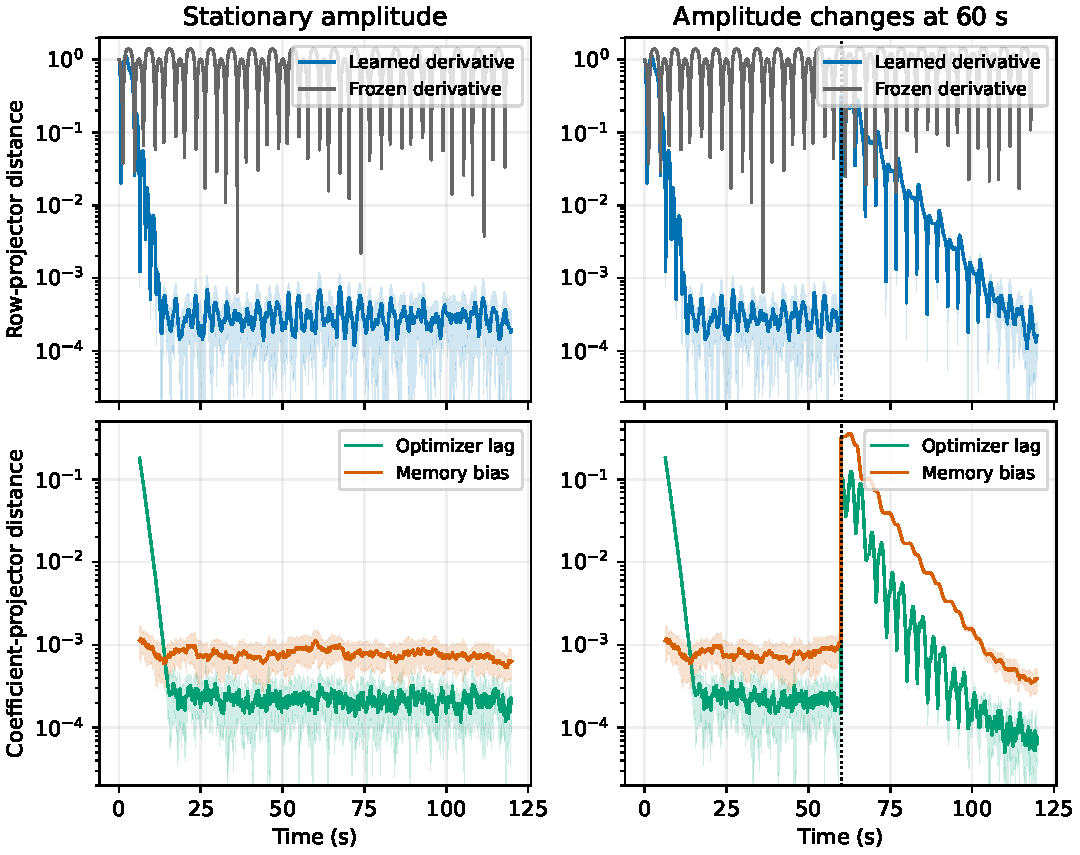
\includegraphics[width=\textwidth]{direct_lift_diagnostics}
 \caption{Direct lifted rate-field learning, all ten seeds per scenario.
 Lines show the across-seed mean and shading shows one sample standard
 deviation, displayed on logarithmic axes. Upper panels compare evaluated
 row-projector error for the learned and frozen fields. Lower panels
 separate coefficient optimization lag from empirical-memory bias.
 The vertical dotted line marks the amplitude change. Lower panels begin
 after one phase cycle; every fifth sample is displayed, while all samples
 in the declared windows enter the statistics.}
 \label{fig:direct_lift_diagnostics}
\end{figure*}

Table~\ref{tab:direct_lift_results} reports time means for each seed and
then mean $\pm$ sample standard deviation across all ten seeds. In
$[100,120)$~s, the learned physical row-projector error is
$(2.940\pm0.320)\times10^{-4}$ for the stationary case and
$(5.187\pm0.744)\times10^{-4}$ after the jump. In the jump window
$[60,80)$~s it is $(9.330\pm0.007)\times10^{-2}$: the estimator does
not instantaneously acquire the changed derivative. In the same window,
the coefficient memory bias exceeds the optimizer lag, consistent with
retaining incompatible pre-change data. These are observations for this
protocol, not a theorem about arbitrary changes or noise models.

Across all recorded samples and seeds, the minimum evaluated row norm is
0.670324 for the stationary case and 0.529792 for the jump case; no
zero-row or nonfinite projector was observed. The maximum coefficient
unit-norm deviation is $3.34\times10^{-16}$, rounded upward. No
increase in the frozen-memory quadratic energy was recorded during an
adaptation step. These sampled checks do not turn coefficient
normalization into a general phase-uniform rank certificate.

The public postprocessor \path{experiments/plot_direct_lift_audit.py}
independently checked the original file hashes, reconstructed all
120,020 recorded rows from the twenty runs, rebuilt every stored moment,
and recomputed the reported field projectors, energies, norms, and
window statistics. It also checked 280 fixed-index transitions using
direct matrix exponentials, independently of the simulation's spectral
implementation. Raw records, protocol, source snapshot, environment,
and hashes remain a separately identified reproduction artifact; the
supplement contains only the generated figure and table.

This experiment supports direct adaptation of an evaluated differential
row space from tangent observations without derivative-entry targets.
Its scope remains a known harmonic basis, exact clock/phase, one initial
coefficient row, one stationary amplitude and one prescribed jump, and
sensor-noise variation. It does not establish frequency discovery,
generalization to unrelated trajectories, or closed-loop performance.

\subsection{Exact-Jacobian companion with every coefficient adaptive}
\label{sec:direct_jacobian_companion}
A separately declared companion, \texttt{direct\_jacobian\_20261118\_v1},
tests the additional integrability restriction that every candidate row be
an exact Jacobian, not just a rate-product field. This is a different
restriction from direct learning without supplied physical partial algebra;
its prescribed residual family is
\begin{align}
 f_q(x,y)&=q_0x+q_1y+q_2\sin x+q_3\cos x,\\
 F_q(x,y)&=(q_0+q_2\cos x-q_3\sin x,\ q_1),
 \label{eq:direct_jacobian_family}\\
 \psi_J&=\col(v_1,v_2,\cos x\,v_1,-\sin x\,v_1).
\end{align}
All four coefficients adapt, including $q_1$; no derivative entry is
held at its true value. The clock rate $v_1=1$ is an observed context
channel, not a fixed learned derivative coefficient. The learner uses
$q\psi_J=F_qv_m$ and the same normalized update
(\ref{eq:direct_step}), with a $4\times4$ memory. It receives no residual
level and no derivative-entry targets. The derivative is exact at fixed
$q$ for every iterate; an adapting residual still has the parameter term
in its total time derivative.
After the jump, the continuous physical level in
(\ref{eq:direct_piecewise_level}) includes the additive offset
$(A_1-A_2)\sin x_c$. That constant is absent from this candidate basis,
is not learned, and is not used: its derivative is zero, so the physical
Jacobian remains representable on each segment.

The stationary/jump schedules, step, memory, gain, noise, durations, and
twenty seed/scenario combinations are unchanged. The separately fixed
initial row is $(0.3,1,-0.3,0.2)$ normalized to unit length. This
four-dimensional family and initialization were declared before its runs;
the six-dimensional protocol and records were preserved. A trace-level
comparison confirmed that all twenty tangent observation streams match
their six-dimensional counterparts exactly. The families have different
constraints and initial rows, so their numerical differences are not a
comparison of estimators with matched capacity.

\begin{directproposition}[Exact Jacobians and clean identifiability]
\label{prop:direct_jacobian_identifiability}
For every $q\in\mathbb R^4$, (\ref{eq:direct_jacobian_family}) is
$D_zf_q$ and $q\psi_J=F_qv$. For every constant real $A$, the
clean full-period covariance of $\psi_J$ has eigenvalues
\begin{equation}
 \{0,\tfrac12,1,\tfrac{1+A^2}{2}\}
\end{equation}
and its kernel is spanned by $(0,1,A,0)$.
\end{directproposition}
\begin{IEEEproof}
Differentiate $f_q$ with respect to $x$ and $y$ while holding $q$ fixed;
substitution gives the tangent-product identity. With
$v=(1,-A\cos x)$, the clean incompatibility is
$q_0+(q_2-Aq_1)\cos x-q_3\sin x$.
Independence of these three harmonics gives the stated kernel.
The constant and sine coordinates have covariance eigenvalues $1$ and
$1/2$. The remaining block is
$\frac12\left[\begin{smallmatrix}A^2&-A\\-A&1\end{smallmatrix}\right]$,
whose eigenvalues are $0$ and $(1+A^2)/2$.
\end{IEEEproof}
Unlike the larger rate-field family, the exact-Jacobian family retains a
one-dimensional clean kernel even at $A=0$. This difference comes from
the integrability restriction and smaller candidate space. It does not
establish robustness for arbitrary features or sensing assumptions.

\begin{table*}[t]
\centering
\caption{Exact-Jacobian companion: mean $\pm$ sample standard deviation across all ten seeds per scenario, after averaging each pre-update diagnostic over its half-open time window. Every candidate is an exact Jacobian and all four coefficients adapt.}
\label{tab:direct_jacobian_results}
\begin{tabular}{llcccc}
\toprule
Scenario & Window (s) & Learned derivative & Frozen derivative & Optimizer lag & Memory bias\\
\midrule
Stationary & 40--60 & $(2.479\pm0.728)\times10^{-4}$ & $(9.075\pm0.000)\times10^{-1}$ & $(4.123\pm0.266)\times10^{-5}$ & $(3.373\pm1.061)\times10^{-4}$\\
Stationary & 60--80 & $(2.529\pm0.693)\times10^{-4}$ & $(9.022\pm0.000)\times10^{-1}$ & $(4.163\pm0.365)\times10^{-5}$ & $(3.244\pm0.890)\times10^{-4}$\\
Stationary & 100--120 & $(2.631\pm0.456)\times10^{-4}$ & $(8.870\pm0.000)\times10^{-1}$ & $(4.108\pm0.320)\times10^{-5}$ & $(3.553\pm0.592)\times10^{-4}$\\
\midrule
Jump & 40--60 & $(2.479\pm0.728)\times10^{-4}$ & $(9.075\pm0.000)\times10^{-1}$ & $(4.123\pm0.266)\times10^{-5}$ & $(3.373\pm1.061)\times10^{-4}$\\
Jump & 60--80 & $(8.872\pm0.007)\times10^{-2}$ & $(1.042\pm0.000)\times10^{0}$ & $(3.974\pm0.004)\times10^{-3}$ & $(9.678\pm0.008)\times10^{-2}$\\
Jump & 100--120 & $(4.825\pm0.712)\times10^{-4}$ & $(1.034\pm0.000)\times10^{0}$ & $(3.476\pm0.253)\times10^{-5}$ & $(5.290\pm0.596)\times10^{-4}$\\
\bottomrule
\end{tabular}
\end{table*}

All twenty companion runs and all 120,020 recorded rows were audited
independently, including complete memory reconstruction and another
280 transitions checked with direct matrix exponentials. Three focused
tests additionally check finite-difference Jacobians for arbitrary
coefficients, the covariance spectrum, and the tangent-feature identity.
The minimum evaluated row norm over every seed and sample is 0.509438;
no invalid row projector or frozen-memory energy increase was recorded,
and the largest unit-norm deviation is $2.23\times10^{-16}$, rounded up.

The learned physical row-projector error in $[100,120)$~s is
$(2.631\pm0.456)\times10^{-4}$ for the stationary case and
$(4.825\pm0.712)\times10^{-4}$ after the jump. During $[60,80)$~s
after the jump it is $(8.872\pm0.007)\times10^{-2}$.
Table~\ref{tab:direct_jacobian_results} includes the frozen baseline,
optimizer lag, and empirical-memory bias using the same gauge-invariant
definitions as above. Thus this companion supplies numerical evidence of
coefficient-induced Jacobian row-space recovery within its prescribed
family, with every coefficient adaptive and every candidate integrable.
It is not independent-entry partial learning with unknown algebraic structure.
The evidence remains confined to the declared family, observations,
initialization, and two amplitude schedules. Additive levels remain
unidentified, and no control or generalization claim is added.

\section{Supplementary matched-family estimator comparison}
\label{sec:estimator_comparison}
This additional experiment compares numerical estimators within the prescribed
Fourier feature family. It is separate from both the original structured-study
records and the retained normalized periodic-plant protocol.
The protocol and all ten seeds (10--19) were fixed before examining comparison
outcomes. Plant, reference, initial state, known phase, measurement noise,
integration, sampling, secant window, coefficient convention, coefficient box,
and feature scales are exactly those of the bounded Fourier protocol in
Section~\ref{sec:fourier_protocol}. Every
method uses all six $K=1$ coefficients and the supplied coefficient of $-u$ is
fixed at one. Thus this comparison does not give an alternative method a smaller
feature family or withhold the phase from it.

\subsection{Three estimators and two data regimes}
The original method takes eight projected-gradient steps per observation on
the exponentially weighted covariance objective, with memory time $8$~s and
reciprocal-trace step size. The second method, denoted EWLS, minimizes the
\emph{same} convex quadratic objective over the same coefficient box by bounded
variable least squares. It uses the eigendecomposition square root of the
accumulated covariance and SciPy's BVLS solver~\cite{SciPyBVLS}, tolerance $10^{-10}$ and maximum
100 iterations. Negative covariance eigenvalues attributable to roundoff are
clipped to zero; no ridge penalty is added. The same initial coefficient vector
is used before the first observation. Subsequently EWLS imposes no penalty for
departing from that initial vector; early rank-deficient problems need not have
a unique minimizer. EWLS is an alternative numerical solver for this memory
criterion, not an independently expressive model family.

The third method takes one projected normalized least-mean-square step on the
current observation, with gain one. It keeps the same coefficient scales and
box but does not use past observations in its update. This is a combined
memory-and-update ablation, not a comparison holding memory fixed. For
diagnostics only, its trace also records the common exponentially weighted
covariance; that matrix does not enter its update.

In the primary comparison the original projected-memory controller generates
one trajectory per seed, and all three estimators receive the identical observed
complete-feature secants. Their current models are scored before assimilating
the current secant. Their different differential errors therefore reflect
estimators operating on the same data. The task error and applied input of that
common trajectory belong to its generating controller, and are not attributed
to the two shadow estimators. In a separate comparison, EWLS and instantaneous
NLMS each control their own trajectory, with the same per-seed noise draws and
otherwise unchanged protocol. These branches compare closed-loop task
performance but no longer have identical regressors. The original controller's
primary trajectory supplies its own closed-loop branch.

The learner input is only the noisy observed complete-feature secant. Clean
rates, true coefficients, and true partial derivatives are evaluator-only.
No derivative target, desired control target, or future sample is supplied to
an update. All methods use the same known-frequency family and calibrated
zero implicit level. The final sample is scored without a coefficient update;
the common observation routine still updates its diagnostic memory.

\subsection{Objective identity and single-sample descent}
Write the scaled observed implicit channel as $v_i=(a_i^\top,b_i)^\top$,
the scaled coefficient row as $q(\theta)=(\theta^\top,1)$, and the feasible
coefficient box as $\mathcal C$. With $\beta=\exp(-\Delta t/8)$ and $R_0=0$,
the covariance recursion gives
\begin{equation}
 J_n(\theta)=\frac12q(\theta)R_nq(\theta)^\top
 =\frac{1-\beta}{2}\sum_{i=1}^n\beta^{n-i}
       [q(\theta)v_i]^2.
\end{equation}
This equality follows by substitution in
$R_n=\beta R_{n-1}+(1-\beta)v_nv_n^\top$ and induction.
Every retained sample is therefore evaluated at the same current candidate;
the criterion is not an accumulation of stale fitted residuals. If
$R_n=U\Lambda U^\top$ with $\Lambda\succeq0$, then
$B=\Lambda^{1/2}U^\top$ gives
$J_n(\theta)=\|Bq(\theta)^\top\|^2/2$. The bounded least-squares
problem solved by EWLS is consequently the same covariance minimization
problem, up to floating-point factorization and solver tolerance. Positive
definiteness of its free-coefficient Hessian gives uniqueness; positive
semidefiniteness alone does not. A small numerical optimality residual certifies
this constrained optimization problem, not physical identification in noisy
regressors.

For the instantaneous method let
$\ell_n(\theta)=[q(\theta)v_n]^2/2$,
$L_n=\|a_n\|^2$, and
$\eta_n=1/\max(L_n,10^{-12})$. Its update is
\begin{equation}
 \theta^+=\Pi_{\mathcal C}\{
   \theta-\eta_n a_n[q(\theta)v_n]\}.
\end{equation}
For a feasible $\theta$, the projection inequality with
$d=\theta^+-\theta$ gives
$\nabla\ell_n(\theta)^\top d\le-\|d\|^2/\eta_n$.
Expanding the quadratic and using
$(a_n^\top d)^2\le L_n\|d\|^2$ yields
\begin{equation}
 \ell_n(\theta^+)-\ell_n(\theta)
 \le-\left(\frac1{\eta_n}-\frac{L_n}{2}\right)\|d\|^2
 \le-\frac{\|d\|^2}{2\eta_n}.
\end{equation}
This is descent for the just-assimilated sample. It does not ensure small
pre-update error on a later sample, descent of the memory criterion, parameter
identification, or stability of the closed loop.

\subsection{Metrics and limitations}
All reported averages use $60\le t<80$~s and include every planned seed.
In addition to the full scaled differential error, the comparison reports
the relative error restricted to the learned columns $(x,\dot x,\phi)$,
excluding the supplied exact input partial $-1$. The phase column is
included in both errors, and its absolute RMSE is recorded separately.
The trace also contains pre-update sampled energy, clean evaluator energy,
scaled row-projector error, coefficient error, covariance eigenvalues,
box activity, numerical optimality diagnostics, and solver status. Task RMSE
and input RMS are compared only for the respective own-trajectory branches.
Noise corrupts regressors, and successive secants overlap: neither an exact
memory minimizer nor a small training criterion removes these statistical
limitations. These simulations are not a held-out generalization study or an
exhaustive comparison with other representation-learning methods.

\begin{table*}[t]
\centering
\caption{Same-stream Fourier estimator comparison, mean $\pm$ sample SD over ten seeds on $[60,80)$~s. All three estimators observe the original memory-PG controller trajectory. Differential errors include the phase column; the learned-column error excludes the supplied exact input partial.}
\begin{tabular}{lcccc}
\toprule
Estimator & Full $e_F$ (\%) & Learned columns (\%) & Phase RMSE ($10^{-3}$) & Energy ($10^{-4}$)\\
\midrule
Memory PG & $0.68713\pm0.01883$ & $0.85515\pm0.02348$ & $0.12175\pm0.01134$ & $5.96031\pm0.22187$\\
Memory EWLS & $0.68735\pm0.01884$ & $0.85542\pm0.02349$ & $0.12645\pm0.01095$ & $5.96037\pm0.22205$\\
Instantaneous NLMS & $9.96974\pm0.20244$ & $12.39894\pm0.25955$ & $16.02182\pm0.82651$ & $10.56759\pm0.51017$\\
\bottomrule
\end{tabular}
\label{tab:estimator_same_stream}
\end{table*}

\begin{table}[t]
\centering
\caption{Separate closed-loop Fourier trajectories, mean $\pm$ sample SD over ten seeds on $[60,80)$~s. The memory-PG branch is the primary generating trajectory; EWLS and NLMS each control their own trajectory.}
\setlength{\tabcolsep}{4pt}
\begin{tabular}{lcc}
\toprule
Controller & Tracking RMSE ($10^{-3}$) & Input RMS\\
\midrule
Memory PG & $2.29896\pm0.03121$ & $0.644832\pm0.000046$\\
Memory EWLS & $2.29931\pm0.03131$ & $0.644831\pm0.000046$\\
Instantaneous NLMS & $33.09200\pm2.75300$ & $0.607014\pm0.003725$\\
\bottomrule
\end{tabular}
\label{tab:estimator_closed_loop}
\end{table}


\begin{figure*}[t]
\centering
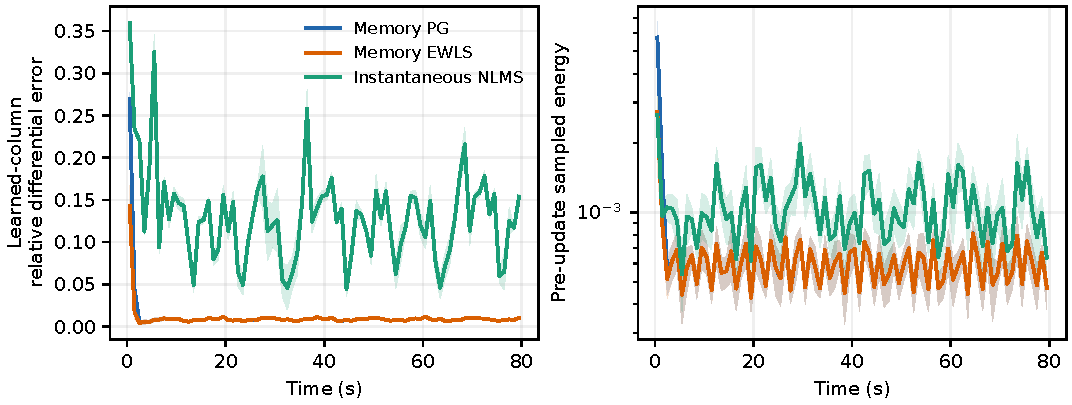
\includegraphics[width=.98\textwidth]{estimator_common_stream.pdf}
\caption{Same-stream comparison over all ten seeds. Each trace first averages
within nonoverlapping one-second bins; lines and shading are then the mean
and sample SD across seeds. The differential metric excludes the supplied
exact input partial. The two memory methods nearly overlap; instantaneous
NLMS uses the same feature family but a different memory/update rule.}
\label{fig:estimator_common_stream}
\end{figure*}

\begin{figure*}[t]
\centering
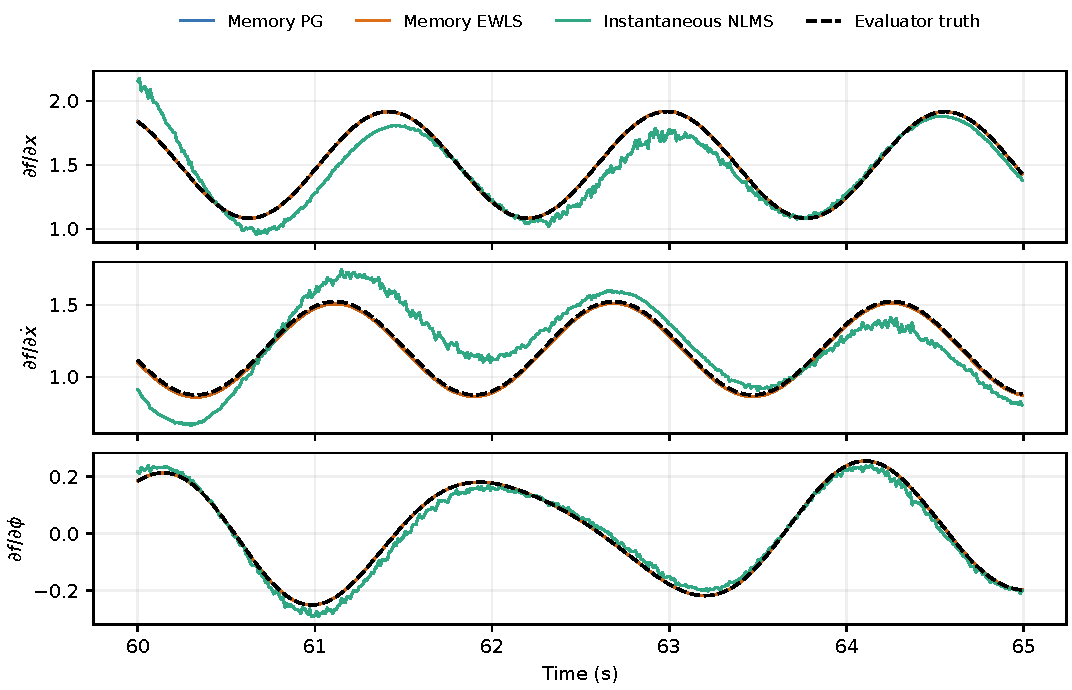
\includegraphics[width=.98\textwidth]{estimator_partial_tracking.pdf}
\caption{Evaluated learned partials on the preselected seed-10 common stream,
shown on $[60,65)$~s without smoothing. All estimates are evaluated at the same
plant context before assimilating the current secant. The input partial $-1$
is supplied and is therefore omitted. Dashed evaluator truth is never given
to a learner. The phase column includes differentiation of the complete
harmonic--state products; it is not a coefficient-only error.}
\label{fig:estimator_partial_tracking}
\end{figure*}

Tables~\ref{tab:estimator_same_stream}--\ref{tab:estimator_closed_loop} and
Figures~\ref{fig:estimator_common_stream}--\ref{fig:estimator_partial_tracking}
show that the original projected-memory method and the matched EWLS optimizer
have very similar late-window outcomes in this experiment. This does not
establish their equivalence in other regimes or an advantage of the proposed
update over exact quadratic optimization. Instantaneous NLMS has larger
differential and task errors here. Its gain was fixed at one before the runs;
this comparison changes both memory and update and does not establish an
advantage over a tuned LMS or recursive least-squares family.

Every planned run completed: 30 plant trajectories produce 50 estimator
traces, with no solver failures. An independent audit recomputed differential
metrics, clock columns, pre-update scores, covariance objectives, and every
projected-gradient/NLMS update from the CSV observations and coefficients.
For EWLS, the largest infinity norm of the projected optimality residual
after an update was $4.7\times10^{-15}$. This statistic excludes the final
scored observation, which deliberately has no parameter update. On the
common streams, the largest positive difference between the EWLS and
projected-gradient post-update memory objectives was
$1.9\times10^{-19}$, attributable to roundoff. The common late-window mean
minimum free-coefficient covariance eigenvalue was
$0.0480006\pm0.0000073$, and mean spectral condition number was
$3.77363\pm0.00037$. These are observed noisy covariance diagnostics, not a
certificate of physical persistent excitation.

Recorded cumulative observation/update-call times per 80-second common-stream
run were $2.165\pm0.091$~s for projected memory gradient,
$3.127\pm0.134$~s for EWLS, and $2.016\pm0.082$~s for instantaneous NLMS.
These descriptive timings include the common covariance diagnostics even
for NLMS, whose update does not use them; they exclude plant integration,
evaluation, and file output. Other computations ran on the same machine,
so these measurements are not a controlled runtime benchmark.

\section{Full-record reproduction and learned-partial diagnostics}
\label{sec:reproduction_audit}

\subsection{Historical records versus new executions}
The original all-seed archives named in \texttt{docs/DATA\_MANIFEST.json}
could not be located. Their recorded checksums do not make them available.
The repository did retain every original structured-study and paired-transfer
summary, along with the ten structured-study and two transfer traces for seed~10.
We therefore executed the unchanged declared protocols again, preserving
the historical records and using separate output directories. These are
newly reproduced simulation records, not recovered original archives.
The historical reconstruction status of contact and Burgers is unchanged.

The reproduction uses an immutable snapshot of the simulation sources and
configurations from repository commit
\texttt{374187a31d69e9c93eded1bbc8440696804364b9}.
Source hashes were checked against that commit before comparing outcomes.
The runner records the invocation, all seeds, configurations, package
versions, platform, random-generator identity and states, per-run status,
and file hashes. Two worker processes and one numerical-library thread per
worker were used. The execution environment is Python~3.12.3,
NumPy~2.3.5, SciPy~1.17.0, and Matplotlib~3.10.8; the historical metadata
records Python~3.13.5. Thus identical environment provenance is not claimed.

All 120 declared runs completed, with no failed or excluded seeds:
100 original structured-study runs and 20 paired-transfer runs. The independent audit
passed 7,851 checks. Every regenerated per-run summary and the main and
transfer aggregate tables matched their saved historical counterparts
numerically; the maximum absolute difference was zero. All twelve
previously available raw-run arrays also matched numerically with
maximum absolute difference zero. These agreements do not establish
byte identity with either missing historical ZIP, whose original
contents were unavailable. No historical record or value was overwritten;
the retained normalized periodic-plant experiment has separately identified records.


The audit recomputes task errors, evaluated partials, compatibility
energies, aggregation windows, sample standard deviations, saturation,
and frozen-model checks from the generated records. Contact integral
energies and Fourier complete-feature energies are additionally
reconstructed from their declared sensor-noise streams. Existing
overwrite-prone summarization scripts are not invoked. Comparisons use
relative tolerance $10^{-9}$ and absolute tolerance $10^{-11}$;
the reported maximum differences describe the actual observations, not
merely acceptance within tolerance.

The original scripts record time-step diagnostics and selected partial or
field snapshots, rather than every noisy sensor vector. For example,
Burgers field snapshots are spaced by $0.1$~s. The retained executable
source, configurations, seeds, and PCG64 generator states specify how to
regenerate the full sensing sequence. The new estimator comparison also
saves its observed rate stream explicitly. This distinction prevents
calling a diagnostic trace a complete original sensor log.

Separate regenerated structured-study and excitation archives contain source,
configuration, execution, audit, and checksum evidence with their records.
Their names and hashes are recorded in
\texttt{docs/REPRODUCTION\_20261118.json}; the old archive manifest is
preserved. These are local artifacts at this revision, not an asserted
public release or permanent data deposit. New comparison and direct-lift
records have separate protocol identities and do not overwrite any historical
statistic. Their local archive is described in
\path{docs/SUPPLEMENTARY_STUDIES_20261118.json}, including the comparison,
both direct-learning studies, and learned-partial postprocessing.
The retained normalized periodic-plant Fourier experiment has its own records and archive,
described in Section~\ref{sec:normalized_fourier_results} and
\path{docs/NORMALIZED_FOURIER_20261118.json}. The current direct-field
main experiments have separate identities and records in
Section~\ref{sec:direct_main}.

\subsection{Errors on coefficient-dependent partial entries}
The full-matrix error used in the original experiments includes supplied
derivative entries in its denominator. To distinguish estimation from
correct supplied structure, we also evaluate $e_{F,U}$ in
(\ref{eq:audit_unknown_only}) on every reproduced run. Contact excludes
the supplied $\rho$, unit and fixed-zero entries; Fourier excludes the
input partial $-1$; Burgers excludes the unit $w_t$ partial. The original
context and row scalings are retained. All remaining true denominators
are nonzero in these records, and supplied blocks were checked to be
identical between the estimated and true matrices. ``Learned entries'' in
the retained diagnostic labels means coefficient-dependent evaluated
entries; it does not mean that those entries were independent learner
states. Excluding supplied entries from a metric changes its denominator,
not the underlying learning rule.

\begin{table*}[t]
\centering
\caption{Reproduced original protocols: late-window evaluated-partial
errors, mean $\pm$ sample standard deviation across all ten seeds.
Contact uses $[100,120)$~s, Fourier $[60,80)$~s, and Burgers $[18,24)$~s.
Contact and Burgers use saved $0.1$-s partial snapshots; Fourier uses all
$0.01$-s records. Consequently snapshot averages need not equal the
original all-step means. Different physical scalings prevent interpreting
the rows as a comparison of difficulty across systems.}
\label{tab:unknown_partials}
\begin{tabular}{llcc}
\toprule Study & Method & All entries & Learned entries \\
\midrule
Contact & learned & $0.000896\pm0.00043$ & $0.000915\pm0.00044$ \\
Contact & frozen & $0.584\pm7.8\times10^{-7}$ & $0.596\pm7.5\times10^{-7}$ \\
Contact & oracle & $0\pm0$ & $0\pm0$ \\
Fourier & learned & $0.00687\pm0.00019$ & $0.00855\pm0.00023$ \\
Fourier & K0 & $0.185\pm8.6\times10^{-6}$ & $0.224\pm1\times10^{-5}$ \\
Fourier & frozen & $0.214\pm2.9\times10^{-17}$ & $0.26\pm5.9\times10^{-17}$ \\
Fourier & oracle & $0\pm0$ & $0\pm0$ \\
Burgers & learned & $0.000108\pm9.7\times10^{-6}$ & $0.000147\pm1.3\times10^{-5}$ \\
Burgers & frozen & $0.159\pm0$ & $0.217\pm0$ \\
Burgers & oracle & $0\pm0$ & $0\pm0$ \\
\bottomrule
\end{tabular}

\end{table*}

\begin{figure*}[t]
\centering
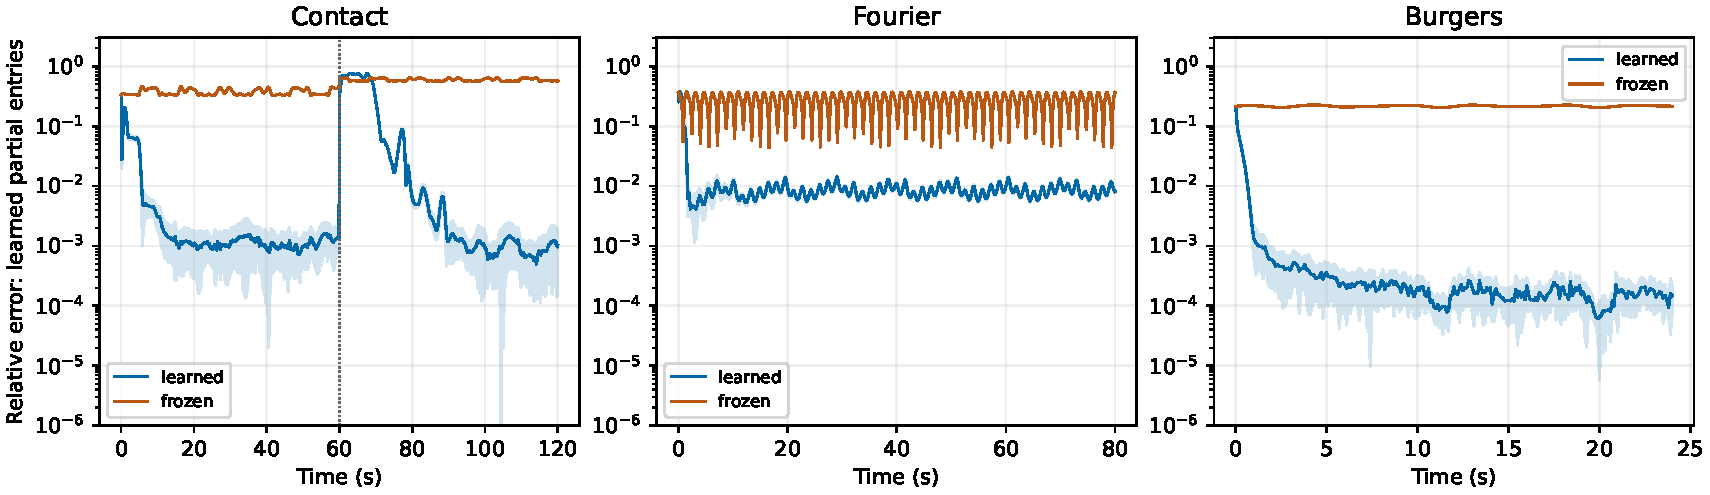
\includegraphics[width=.98\textwidth]{unknown_partial_tracking.pdf}
\caption{Original structured protocols: error restricted to learned partial entries on each controller's
own trajectory. Lines are ten-seed means and shading is one sample
standard deviation; no temporal smoothing is applied. The contact change
occurs at $60$~s. The logarithmic display range does not modify recorded
errors; exact oracle curves are omitted from this plot and retained in
Table~\ref{tab:unknown_partials}. The Fourier panel uses the bounded
six-coefficient protocol, distinct from both the retained normalized
periodic-plant study and the current direct-field main benchmark.}
\label{fig:unknown_partial_tracking}
\end{figure*}

These diagnostics directly test the evaluated derivatives on the observed
contexts, including contact recovery after changed material and actuation
and the varying Fourier phase column. They do not turn a prescribed-family
fit into unrestricted Jacobian discovery. The stationary Fourier
coefficients can generate rapidly changing derivatives, whereas contact
requires the coefficients themselves to adapt after the change. Both
effects should be distinguished from optimization progress alone.
The online data remain dependent on the controller and prior updates;
frozen transfer and evaluator-only query tests in Section~\ref{sec:excitation}
address a separate, narrower form of reuse.

% Separately identified normalized-law experiment. The parent build supplies
% the generated table and figures after auditing the executed records.
\section{Coupled normalized learning in the periodic plant}
\label{sec:normalized_fourier_results}
% Audit SHA-256: 195a72fc6b9fd544832f830d537bc885f7ee06d4b61f9f3e68acc61b9e20350b
\begin{table*}[t]
\centering
\caption{Retained normalized periodic-plant protocol: mean $\pm$ sample standard deviation over seeds 10--19, using $60\le t<80$~s. Every numeric column is multiplied by $10^3$. $e_P$ is evaluated differential projector error; $e_F$ uses learned-input gauge alignment. Dashes mark shadows without their own control trajectory.}
\label{tab:normalized_fourier_results}
\begin{tabular}{llrrrr}
\toprule
Stream & Estimator & $10^3 e_P$ & $10^3 e_F$ & $10^3$ phase RMSE & $10^3$ tracking RMSE \\
\midrule
Replay & Normalized flow & $6.256\pm0.167$ & $5.487\pm0.160$ & $0.350\pm0.019$ & --- \\
Replay & Memory minimum & $6.357\pm0.161$ & $5.590\pm0.156$ & $0.337\pm0.017$ & --- \\
Replay & Frozen prior & $247.986\pm0.003$ & $218.876\pm0.002$ & $125.018\pm0.010$ & --- \\
Flow-controlled & Normalized flow & $6.216\pm0.165$ & $5.451\pm0.159$ & $0.351\pm0.019$ & $2.311\pm0.029$ \\
Flow-controlled & Memory minimum & $6.317\pm0.159$ & $5.552\pm0.154$ & $0.338\pm0.017$ & --- \\
Flow-controlled & Frozen prior & $248.065\pm0.002$ & $218.926\pm0.001$ & $125.254\pm0.006$ & --- \\
\bottomrule
\end{tabular}
\end{table*}

This retained historical Fourier experiment applies the normalized covariance
learning law to
the periodic plant, with all seven homogeneous coefficients adaptive.
It is identified as \path{normalized_fourier_coupled_20261118_v1}.
The earlier Fourier study instead fixes the input coefficient and takes
bounded projected-gradient steps on six free coefficients. Its statistics
remain unchanged in Section~\ref{sec:fourier_protocol}. The present records
demonstrate normalized coefficient learning and calibrated control readout
within the stated family. The retained contact and Burgers protocols use
separate structured updates. The current direct-field main experiments are
documented in Section~\ref{sec:direct_main}. This is a retained
coefficient-family demonstration: the update is normalized, but the learner
is given the physical algebra that maps its coefficients to partials.
It therefore does not satisfy the direct all-entry requirement in
Section~\ref{sec:scope}. Nor does comparing the known phase frequency with
the desired reference establish faster partial variation than the actual
applied input; that signal comparison is not demonstrated by these records.

\subsection{An exact-Jacobian family with a learned input partial}
For context $z=(x,r,u,\phi)$, let $h=(1,\cos\phi,\sin\phi)^{\mathsf T}$,
$h'=(0,-\sin\phi,\cos\phi)^{\mathsf T}$, and define
\begin{equation}
 \zeta(z)=\col(hr,hx,-u),\qquad
 S=\operatorname{diag}(1,.3,.3,1,.4,.4,1).
 \label{eq:nf_features}
\end{equation}
The learned row satisfies $q\in\mathbb R^{1\times7}$, $\|q\|=1$.
Write $a=qS=(a_\rho,a_\kappa,a_u)$ with two three-entry blocks. Then
\begin{equation}
 f_q(z)=qS\zeta(z)=(a_\rho h)r+(a_\kappa h)x-a_u u,
 \label{eq:nf_family}
\end{equation}
and its exact fixed-parameter Jacobian is
\begin{equation}
 F_q(z)=\bigl(a_\kappa h,\ a_\rho h,\ -a_u,
                 (a_\rho h')r+(a_\kappa h')x\bigr).
 \label{eq:nf_jacobian}
\end{equation}
Thus every candidate is integrable and the clock partial includes both
complete-product terms. The input coefficient $a_u$ is learned, not fixed.
There are no coefficient boxes, ridge terms, or derivative-entry targets.
Normalization is imposed in the declared $S$ coordinates; changing those
units changes the estimator. The physical initial prior
$(1,0,0,1,0,0,1)$ is multiplied by $S^{-1}$ and normalized to obtain $q_0$.
True coefficients and clean rates enter only the plant and evaluator.
This information boundary excludes derivative-target leakage; it does not
remove the supplied physical structure of $\zeta$.

Sampling is $\Delta t=.01$~s, and the measured channel is
\begin{equation}
 w_n=\frac{S[\zeta_m(t_n)-\zeta_m(t_n-.05)]}{.05}.
 \label{eq:nf_secant}
\end{equation}
This complete-feature secant includes held-command jumps; it is not a
measured instantaneous raw-context tangent. For a smooth context it averages
the complete derivative at fixed $q$. Across command jumps no ordinary
smooth-path argument is presumed. The true clean residual vanishes at both
endpoints, so its homogeneous row also annihilates their feature difference.
The supplied harmonic family, phase $\phi=4t$, exact state and command,
and rate-noise standard deviation $.001$ are retained assumptions.

\subsection{Integration of the coupled normalized law}
With $R_0=0$, memory $\tau=8$~s and gain $\eta=1$, the learner integrates
\begin{equation}
 \dot R=ww^{\mathsf T}-R/\tau,\qquad
 \dot q=-\eta\bigl(qR-(qRq^{\mathsf T})q\bigr).
 \label{eq:nf_coupled}
\end{equation}
The latest observed $w_n$ is held over the next sample interval. At local
elapsed time $s\in[0,\Delta t]$, the exact memory is
\begin{equation}
 R(s)=e^{-s/\tau}R_n+\tau(1-e^{-s/\tau})w_nw_n^{\mathsf T}.
 \label{eq:nf_memory}
\end{equation}
This is the unnormalized exponential integral. The earlier code's
exponential average differs by the factor $\tau$; silently reusing that
average with the same gain would change (\ref{eq:nf_coupled}).
Gain one was specified before outcomes and is not claimed equivalent to
the earlier eight projected-gradient iterations.

The implementation solves the seven-dimensional linear equation
\begin{equation}
 \dot y(s)=-\eta R(s)y(s),\qquad y(0)=q_n^{\mathsf T},\qquad
 q_{n+1}=\frac{y(\Delta t)^{\mathsf T}}{\|y(\Delta t)\|}.
 \label{eq:nf_linear}
\end{equation}
To check the connection directly, set $q(s)=y(s)^{\mathsf T}/\|y(s)\|$.
The nonsingular linear evolution keeps nonzero $y$ nonzero, and
$\frac{d}{ds}\|y\|=-\eta(qRq^{\mathsf T})\|y\|$.
Differentiating the normalized row gives exactly the second equation in
(\ref{eq:nf_coupled}). This calculation applies to the evolving $R(s)$,
not only a frozen matrix. Numerically, SciPy DOP853 approximates
(\ref{eq:nf_linear}) with relative tolerance $10^{-9}$ and absolute
tolerance $10^{-11}$; endpoint normalization removes radial roundoff.
It is numerical integration of the coupled law, not an exact numerical
solution or a frozen-memory exponential step.

For $J=qRq^{\mathsf T}/2$, direct differentiation gives
\begin{equation}
 \dot J=-\eta\|qR-(qRq^{\mathsf T})q\|^2
               +\tfrac12q\dot Rq^{\mathsf T}.
 \label{eq:nf_moving_energy}
\end{equation}
Consequently fixed-memory descent does not imply monotone energy when
observations change the memory. All evaluated partials are fixed-parameter
derivatives; differentiating $f_{q(t)}(z(t))$ would additionally include
the parameter-adaptation term.

\subsection{Causal readout and two observation regimes}
The current row commands the plant before the current noisy rate is sensed.
Its secant energy and differential are scored before adaptation. Learning
then advances with the observed secant held for the next interval, while
the plant advances by the retained held-input RK4 rule. The updated row
first affects the next command. No assimilation occurs before a complete
secant window exists or after the final scored sample.

Using the plant and reference of Section~\ref{sec:fourier_protocol}, initial
state $x(0)=.2$, and feedback gain two, the calibrated readout is
\begin{equation}
 r_d=\dot x_d-2(x-x_d),\qquad
 u=\frac{(a_\rho h)r_d+(a_\kappa h)x}{a_u}.
 \label{eq:nf_control}
\end{equation}
This expression is invariant to a common nonzero row scale or sign.
The zero residual level remains supplied calibration: derivative learning
does not identify an omitted additive constant. If $|a_u|<.05$, the
controller uses the original frozen physical prior for that command and
records the fallback; the normalized learning law is unchanged. Since
$\|F_q(z)\|\ge |a_u|$ for every $z$, an inactive guard certifies row rank
and the input readout at that coefficient snapshot for every phase.
It does not establish invariance of the guarded set between sampled commands.

The protocol specifies seeds 10--19 in each of two 80-s branches. In the
replay branch, the normalized learner receives the saved observations of
the earlier projected-gradient controller. Its task trajectory belongs to
that controller. In the own-trajectory branch, the normalized learner
controls the plant and generates new observations. Both branches also
carry a frozen normalized prior and a numerical bottom-eigenvector
estimator as same-stream shadows; neither shadow controls an independent
trajectory. The latter minimizes the same sphere objective using the same
$R$ and $S$, subject to a stated numerical tie tolerance. A bottom-eigenvector
target need not equal the physical coefficient row in noisy observations.
The earlier bounded estimator has a different feasible set and normalization,
so its comparison is not merely a choice of solver for this sphere objective.

\subsection{Using the same learned relation for a current-rate query}
In addition to the command executed during learning, the saved pre-update
representation can answer a different query. Hold the recorded current
state, input, and phase fixed, and compute
\begin{equation}
 \widehat r=\frac{a_u u-(a_\kappa h)x}{a_\rho h}.
 \label{eq:nf_rate_completion}
\end{equation}
This query uses neither the current measured rate nor the true rate; the
clean rate enters only the subsequent error calculation. Both readouts use
the same fitted relation and supplied zero residual level. In these records,
the applied command was already computed by (\ref{eq:nf_control}) from
that same pre-update row. Substitution gives $\widehat r=r_d$ whenever
the controller and rate guards are inactive. Thus its error measures
achieved-rate consistency of the inverse readout, not an independent
prediction task. The rate query
is admitted when $|a_\rho h|/\|q\|\ge .05$, a diagnostic conditioning
guard that does not alter the recorded controller or learning sequence.

Postprocessing all ten own-trajectory records gives late-window current-rate
RMSE $(2.671\pm0.071)\times10^{-3}$, compared with
$0.22161\pm0.00001$ for the frozen prior evaluated on those same contexts
and inputs. Both methods admit all 80,010 full-episode queries; the smallest
normalized learned rate denominator is $.32764$. The statistics use
$60\le t<80$~s and sample standard deviation across seeds. This is
a current-rate consistency check of the previously fitted representation,
not future-state prediction, an independent held-out test, or a separate
frozen-controller trajectory. No simulation or training was rerun for this
query. The postprocessor \path{experiments/plot_normalized_fourier_main.py}
records the query outputs, input-file hashes, denominator checks, and summary
under identity \path{normalized_fourier_main_postprocessing_20261119}.
It also produces the historical periodic-plant Fourier panels solely from the
preselected seed-10 own-trajectory records; the replay figures below remain
separately identified diagnostics.

\subsection{Separate diagnostics, provenance, and scope}
Table~\ref{tab:normalized_fourier_results} summarizes the declared
$60\le t<80$~s window. Coefficient-projector error uses the declared feature
coordinates; evaluated differential projectors use context scales
$(.5,1,1,1)$. Physical partial errors first divide (\ref{eq:nf_jacobian})
by $a_u$ wherever the input guard permits. The resulting input partial is
$-1$ by reporting convention, not because it was fixed during learning.
Raw seven-coordinate traces and input coefficients retain this distinction.
Incompatibility, differential recovery, memory-eigenspace lag, and task error
are separate quantities. Tracking RMSE and effort are attributed only to the
own-trajectory normalized controller.

On its own trajectories, the normalized learner achieved mean differential
projector error $0.00622$ and input-aligned relative differential error
$0.00545$, while the frozen prior's corresponding errors were $0.248$ and
$0.219$. Mean tracking RMSE was $0.00231$ and control RMS was $0.6460$.
The adaptive estimators have similar late errors; these observations do not
establish superiority over the empirical memory minimum. That minimum is
poorly conditioned for input readout early in the episode: its guard fails
for 26--65 replay samples and 18--42 own-stream samples per seed. Those
shadow coefficients remain recorded, and their undefined gauge-aligned
diagnostics are marked missing; no such samples occur in the reporting
window. This transient is one reason its estimation trace is not evidence
of a successful controller.

All twenty specified streams completed, giving sixty estimator traces and
480,060 recorded rows. All seven coefficients changed in every normalized
run, and its controller never invoked the fallback. An independent auditor
reconstructed every observed secant and memory, all pre-update derivatives
and energies, the numerical minimizing rows, and the causal plant/control
sequence. It checked all 159,900 normalized-flow transitions with a separately
implemented nonlinear projected-flow RK4 solver, plus 240 transitions with
a tighter coupled $(q,R)$ solve. Maximum componentwise discrepancies were
$7.78\times10^{-16}$ and $3.34\times10^{-16}$, respectively. Twelve new
mechanism tests include all-coordinate finite differences, noncommuting
memory evolution, evaluator poisoning, and preservation of partial failed
runs. These are numerical consistency checks, not formal verification.
Replaying all 8,001 seed-10 samples with tolerances $10^{-11}$ and
$10^{-13}$ and maximum internal step $.005$~s changed the coefficient
projector by at most $2.23\times10^{-15}$ and the evaluated differential
projector by at most $2.16\times10^{-15}$. This refinement holds the
observed stream fixed; it is not a refined closed-loop plant simulation.

The guard was also checked between samples using an analytic speed bound.
For unit $q$ and positive semidefinite $R$,
\begin{equation}
 \|\dot q\|\le\frac{\eta}{2}
 (\lambda_{\max}(R)-\lambda_{\min}(R)).
\end{equation}
Indeed the squared norm is $\eta^2$ times the variance of the eigenvalues
under weights given by the squared coordinates of $q$, and a variable in
$[a,b]$ has variance at most $(b-a)^2/4$.
The memory in (\ref{eq:nf_memory}) lies on the segment joining its interval
endpoints. By convexity of the largest eigenvalue, define
$L_n=\max\{\lambda_{\max}(R_n),\lambda_{\max}(R_{n+1})\}$ to obtain
\begin{equation}
 \inf_{0\le s\le\Delta t}|q_6(t_n+s)|
 \ge |q_6(t_n)|-\eta\Delta t L_n/2.
\end{equation}
The smallest computed lower bound was $0.3499$, above the $0.05$ guard.
This uses floating-point endpoint spectra and the stated held-sample
equations; it is not an interval-arithmetic certificate or invariance theorem.
Separately reconstructed clean memories had numerical rank six throughout
the reporting window (relative tolerance $10^{-10}$), with minimum gap
$0.3058$, and clean true-row secant residual below $3.06\times10^{-15}$.
These are conditions on the executed trajectories, not a general persistent-
excitation result inferred from a positive noisy covariance.

\begin{figure*}[t]
 \centering
 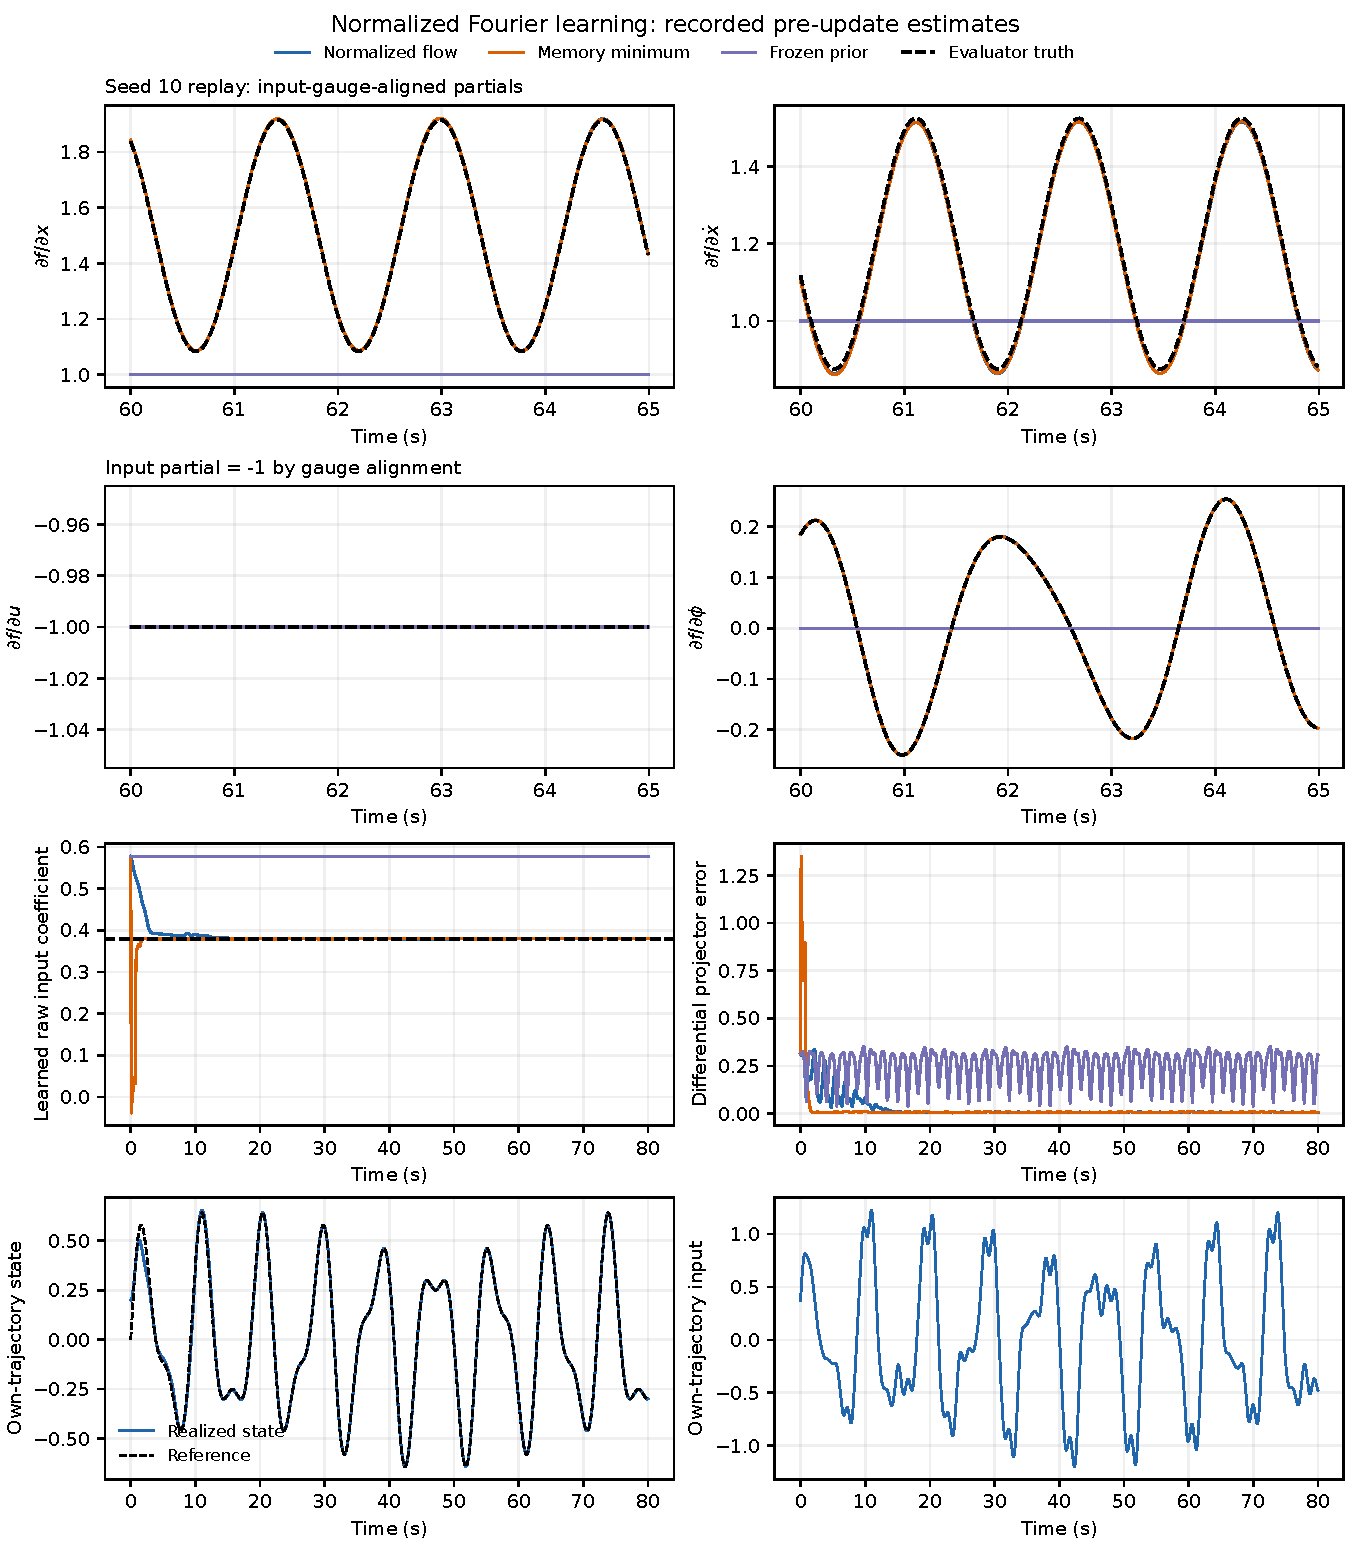
\includegraphics[width=.98\textwidth]{normalized_fourier_partials.pdf}
 \caption{Preselected seed-10 diagnostics, scored before assimilating the
 current secant. The upper four panels compare all three estimators on the
 replay stream over $60\le t<65$~s, a display window within the reporting
 interval.
 Estimates are divided by the learned input coefficient to use the physical
 reporting convention; dashed truth is evaluator-only. The input partial
 becomes $-1$ through this alignment, while all seven coefficients adapt.
 The middle panels show the raw input coefficient and differential projector
 error over the full episode, with every tenth sample displayed. The bottom
 panels alone show the normalized learner's own controlled state and input.
 The clock column includes both complete-product terms.}
 \label{fig:normalized_fourier_partials}
\end{figure*}

\begin{figure*}[t]
 \centering
 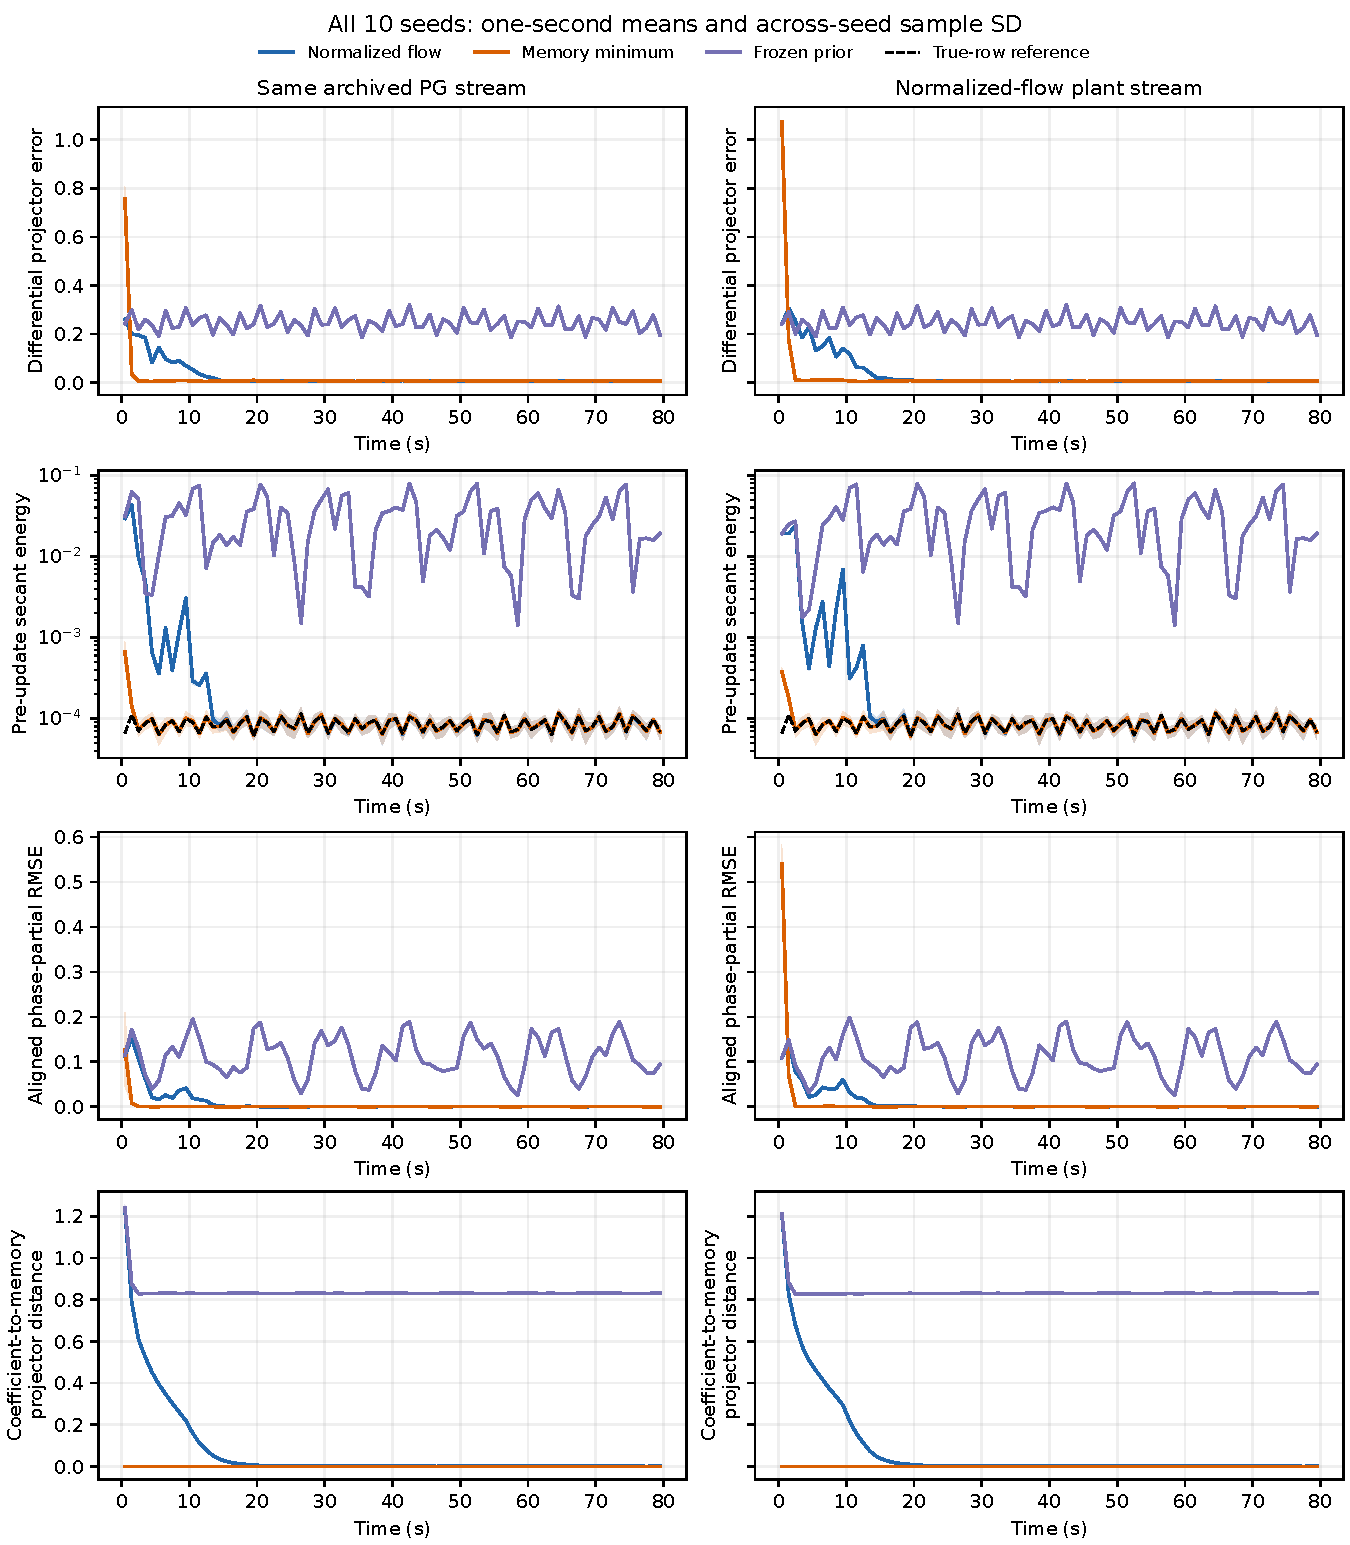
\includegraphics[width=.98\textwidth]{normalized_fourier_summary.pdf}
 \caption{Normalized-learning diagnostics for the replay and own-trajectory
 branches, each specifying ten seeds. Lines and shading show across-seed
 means and sample standard deviations after one-second nonoverlapping
 display aggregation; the phase-error panels use within-bin RMS. All table
 metrics use unsmoothed samples. Undefined startup energies and guarded
 shadow partials are omitted only from their display-bin averages and
 counted in the records; no reporting-window sample is missing. Comparators are same-stream
 bottom-eigenvector and frozen-prior shadows; their traces are not separate
 closed-loop control experiments. Coefficient normalization alone does not
 imply physical identification or successful control.}
 \label{fig:normalized_fourier_summary}
\end{figure*}

The implementation and declared protocol are
\path{experiments/normalized_fourier.py} and
\path{experiments/configs/normalized_fourier_20261118.json};
\path{docs/NORMALIZED_FOURIER_20261118.txt} explains the equations and replay
requirements. Run records contain observed channels, pre/post-update rows
and memories, solver counts, seeds, source/environment snapshots, replay-input
hashes, summaries, and failures, with partial traces retained on simulation
 failure. The executed audit and postprocessor are
 \path{experiments/audit_normalized_fourier.py} and
 \path{experiments/report_normalized_fourier.py}.
 Numerical flow refinement does not test a limit of the sensing period
 or secant window. The archive named in
\path{docs/NORMALIZED_FOURIER_20261118.json} is a local artifact outside
the repository, not a verified public download.

This retained historical demonstration and its diagnostics concern one
known integrable harmonic family
and calibrated readout. Low incompatibility, a positive noisy eigengap, or
accurate integration alone proves neither physical excitation nor closed-loop
stability. Its records are distinct from the earlier bounded comparison, and
it does not establish that the retained coefficient-based contact and Burgers
protocols implement the same normalized law.

\section{Implementation inventory: learning, representation, and readout}
\label{sec:implementation_inventory}
This inventory covers retained historical protocols; the current direct-field
main experiments are documented in Section~\ref{sec:direct_main}.
The simulation evidence has three distinct parts: an estimate changes in
response to observed incompatibility; that estimate represents evaluated
partials; and a readout from the estimate supplies a task command.
Tables~\ref{tab:implementation_main} and
\ref{tab:implementation_support} identify the implemented mechanisms rather
than treating every example as a run of one optimizer. The periodic-plant
experiment in Section~\ref{sec:normalized_fourier_results} integrates the
coupled normalized law. The retained contact and Burgers protocols implement the separately
specified constrained coefficient extension. Their results support learning,
representation, and readout within the stated families, without establishing
that their updates satisfy the normalized-flow convergence hypotheses.
As distinguished in Section~\ref{sec:scope}, these are retained
coefficient-family demonstrations, not the required all-entry direct-field
experiments.

\subsection{Coefficient-induced partials versus directly learned entries}
For a prescribed feature family with all supplied terms retained in the
implicit relation, write
\begin{equation}
 f_\theta(z)=Q_\theta\zeta(z),\qquad
 F_\theta(z)=Q_\theta D_z\zeta(z).
 \label{eq:inventory_representation}
\end{equation}
At a fixed context, a parameter update induces the exact change
\begin{equation}
 \Delta_{\rm learn}F(z)
 =(Q_{\theta^+}-Q_\theta)D_z\zeta(z).
 \label{eq:inventory_partial_update}
\end{equation}
Supplied coefficient entries have zero learning increment. Thus the code
learns residual coefficients and evaluates their induced partials; it does
not directly adapt every partial entry with unknown algebraic structure.
The chain-rule identity does not make these two learning mechanisms
equivalent. Context motion
can also change the evaluated partials even when the coefficients are frozen.
Neither a rapidly varying curve nor coefficient convergence alone establishes
accurate physical partials. The error diagnostics compare estimates and
evaluator truth at the same context, using a declared scale convention.

For the seven-coefficient normalized periodic family, this relation gives
the explicit continuous learning contribution
\begin{equation}
 \left.\partial_t F_q(z)\right|_z
 =-\eta\bigl[qR-(qRq^{\mathsf T})q\bigr]S D_z\zeta(z).
 \label{eq:inventory_normalized_partials}
\end{equation}
Its $F_q$ is (\ref{eq:nf_jacobian}), including both clock-product terms.
Every candidate is an exact Jacobian, and all seven coefficients, including
the input coefficient, adapt. Dividing the displayed partials by that
learned input coefficient is a reporting convention, not a fixed training
coefficient. The generic six-coefficient direct fields in
Sections~\ref{sec:unanchored} and~\ref{sec:direct_lift_results} instead have
$\Delta H(z)=\Delta q\,\Phi(z)$ for their field basis $\Phi$; they need not
be Jacobians and are not covered by (\ref{eq:inventory_representation}).

\begin{table*}[t]
\caption{Retained historical simulation mechanisms. Paths in this table are relative to
\texttt{experiments/}, except the explicitly identified legacy Burgers solver.
The historical normalized Fourier study uses its own controlled trajectory;
replay results are identified separately in
Section~\ref{sec:normalized_fourier_results}.}
\label{tab:implementation_main}
\centering
\setlength{\tabcolsep}{4pt}
\renewcommand{\arraystretch}{1.12}
\begin{tabular}{@{}p{.14\textwidth}p{.29\textwidth}p{.34\textwidth}>{\raggedright\arraybackslash}p{.17\textwidth}@{}}
\toprule
Study & Observations and supplied information & Learned representation and actual update & Simulation and figure code\\
\midrule
Normalized Fourier & Complete-feature secants of $(hr_m,hx,-u)$.
State, input, phase $\phi=4t$, harmonic family, scales, and zero residual
level are supplied; rate measurement is noisy. &
Seven unit-row coefficients $q$; $a=qS$.
Coupled $\dot R=ww^{\mathsf T}-R/8$ and
$\dot q=-\eta[qR-(qRq^{\mathsf T})q]$ are numerically integrated with
changing $R$. The full $F_q$ in (\ref{eq:nf_jacobian}) determines the
learned relation used for command readout and current-rate completion.
No partial column is fixed numerically, but their algebraic dependence
remains prescribed by the residual family.
& \path{normalized_fourier.py};
\path{plot_normalized_fourier_main.py};
\path{report_normalized_fourier.py}.\\[3pt]
Contact & Material integral windows from position and noisy force;
separate measured velocity residuals $v_m-Bu$.
The basis, $\rho=4$, unit rate/velocity coefficients, coefficient boxes,
and zero levels are supplied. Force direction informs the control readout.
& Six material coefficients $(s,a,r,b)$ and four entries of $B$.
Each fit uses 48 projected-gradient steps
(\ref{eq:audit_exact_update}). Material partials are
(\ref{eq:audit_contact_partials}); the kinematic input block is $-B$.
These are integral/level fits, not raw-context tangent normalized flow.
The learned material and actuation estimates enter the contact readout.
& \path{contact.py};
\path{common.py};
\path{make_figures.py}.
Transfer: \path{contact_excitation.py},
\path{plot_excitation.py}.\\[3pt]
Burgers & Spatially averaged complete-feature secants of
$(w_{t,m},ww_s,-w_{ss},-u)$.
Exact state and spectral spatial channels, full actuation, unit $w_t$
coefficient, bounds, and zero level are supplied. &
Three coefficients $(c_a,\nu,b)$; eight scaled projected-gradient steps
(\ref{eq:audit_exact_update}).
$F=(c_aw_s,c_aw,-\nu,-b,1)$.
Both partials of the nonlinear product are represented.
The three learned coefficients enter the inverse control readout;
the discretized family and spatial operators remain prescribed.
& \path{burgers_online.py};
\path{make_figures.py}.
Solver: \path{examples/legacy_suite/simulations/burgers.py}
(repository relative).\\
\bottomrule
\end{tabular}
\end{table*}

\subsection{Updates used by the supporting comparisons}
For the constrained coefficient studies, let $\theta$ denote scaled free
coefficients and $\mathcal W$ their box. Their current-candidate objective
is $J_n(\theta)=\tfrac12\theta^{\mathsf T}H_n\theta+g_n^{\mathsf T}\theta+
\mathrm{const}$, with supplied terms retained in the full implicit row.
The exact memory and projected update are given in
(\ref{eq:audit_exact_update}). The matched EWLS comparison minimizes this
same box-constrained objective; it adds no ridge penalty. The instantaneous
comparison instead takes
\begin{equation}
 \theta^+=\Pi_{\mathcal W}\!\left[
 \theta-\frac{a_n(a_n^{\mathsf T}\theta+b_n)}
 {\max(\|a_n\|^2,10^{-12})}\right],
 \label{eq:inventory_nlms}
\end{equation}
where $(a_n,b_n)$ is the current scaled observed implicit feature channel.
Retaining a covariance for diagnostics does not make this NLMS update a
memory-based estimator.

The Acrobot step is
\begin{equation}
 \theta^+=(I+\eta hH_n)^{-1}(\theta-\eta h g_n).
 \label{eq:inventory_proximal}
\end{equation}
Its memory uses the actual sample weight $h$:
$H_n=\beta H_{n-1}+hV_n^{\mathsf T}V_n$ and
$g_n=\beta g_{n-1}+hV_n^{\mathsf T}k_n$, where $V_n\theta+k_n$
is the complete-feature secant. It is a proximal step, without a persistent
ridge penalty or a positivity projection.

In the active-flow prototype the objective instead contains a ridge term:
\begin{align}
 \theta_n^\star&\in\arg\min_{\theta\in\mathcal W}
 \left[J_n(\theta)+\frac{\lambda_n}{2}
             \|\theta-\theta_0\|^2\right],\\
 \theta^+&=.75\theta+.25\theta_n^\star,
 \label{eq:inventory_flow_relaxation}
\end{align}
with $\lambda_n=10^{-7}\max(\tr G_n/3,10^{-10})$ and $G_n$ the
unregularized feature Gram matrix. These distinctions affect the optimized
criterion and cannot be omitted when relating the experiments to theory.

\begin{table*}[t]
\caption{Supporting mechanisms and source files. In the code column,
E denotes \texttt{experiments/}; L denotes
\texttt{examples/legacy\_suite/simulations/}. The cited sections specify
configurations, records, and metric conventions. A plotting or diagnostic
script does not define an additional learning rule.}
\label{tab:implementation_support}
\centering
\setlength{\tabcolsep}{4pt}
\renewcommand{\arraystretch}{1.10}
\begin{tabular}{@{}p{.14\textwidth}p{.29\textwidth}p{.34\textwidth}>{\raggedright\arraybackslash}p{.17\textwidth}@{}}
\toprule
Study & Observations and adaptive/supplied quantities & Actual update, representation, and readout status & Source / postprocessor\\
\midrule
Original Fourier and estimator comparisons & Same complete features as
the periodic plant; six physical harmonic coefficients adapt, while the
input coefficient is supplied. Phase, family, boxes, and zero level are known.
The $K=0$ ablation learns only two constants. &
Eight projected-gradient steps, box EWLS minimization, or
(\ref{eq:inventory_nlms}), as identified in
Sections~\ref{sec:fourier_protocol} and~\ref{sec:estimator_comparison}.
$F$ is (\ref{eq:audit_fourier_partials}). Same-stream shadows are
distinguished from methods controlling their own trajectories. &
E: \path{fourier_online.py},
\path{estimator_comparison.py};
\path{make_figures.py},
\path{plot_estimator_comparison.py}.\\[3pt]
Acrobot & Complete-feature secants from known positions, velocities and
commands, with noisy acceleration. Five mechanical coefficients adapt;
the actuation column $B=(0,1)^{\mathsf T}$ and mechanical family are supplied.
& Proximal step (\ref{eq:inventory_proximal}).
$F=D_z[M_c(q)\alpha+h_c(q,\dot q)-Bu]$ at fixed $c$.
Identification precedes a separate local LQR episode with the final
coefficients frozen; invalid final models are rejected for readout.
See Figure~\ref{fig:acrobot_archived}. &
L: \path{acrobot.py} generates both records and figures.\\[3pt]
Active-flow prototype & Noiseless full velocity fields and held command;
midpoint fields and secant acceleration form complete-feature differences.
Three coefficients adapt. Spatial operators, geometry, forcing shape,
and acceleration identity are supplied. &
Ridge box solve with 25\% relaxation,
(\ref{eq:inventory_flow_relaxation}).
$F=[c_aDN-\nu L-DK,\ I,\ -b_gB]$.
The adaptive branch continues learning during control; the frozen branch
does not. Differential error probes a specified direction, not a full
operator norm (Section~\ref{sec:afc_prototype}). &
L: \path{airfoil.py} generates records, parameter and control plots.
E: \path{plot_active_flow_fields.py} renders the saved velocity as
vorticity and instantaneous streamlines.\\[3pt]
Reconstructed unanchored Fourier & 4096 noiseless phase/rate samples form
one fixed batch covariance $R$. All six unit-row coefficients adapt;
the harmonic field family and phase are supplied. &
Retracted step $q^+=\operatorname{unit}(q-\alpha g)$,
$g=qR-(qRq^{\mathsf T})q$, with energy/phase-guard backtracking.
$H_q$ need not be a Jacobian. This is a field-learning diagnostic,
without a simulated control episode
(Section~\ref{sec:unanchored}). &
L: \path{fourier.py} generates the checked reconstruction and its figure.\\[3pt]
Direct field and exact-Jacobian companion & Exact phase and one noisy
rate channel; all six field coefficients or all four Jacobian-family
coefficients adapt. The basis is supplied; no derivative entry is fixed.
& $R^+=\beta R+(1-\beta)\psi\psi^{\mathsf T}$, then
$q^+=\operatorname{unit}(qe^{-\eta hR^+})$.
This is a frozen-memory normalized substep.
The six-dimensional $H_q$ need not be integrable; the companion has
$F_q=(q_0+q_2\cos x-q_3\sin x,q_1)$.
Neither study has a controlled plant (Section~\ref{sec:direct_lift_results}).
& E: \path{direct_lift_audit.py},
\path{direct_jacobian_audit.py};
\path{plot_direct_lift_audit.py},
\path{audit_direct_jacobian.py}.\\[3pt]
Additional diagnostics & Existing learned and comparison records;
no new observations or adaptive states. The contact transfer study
uses the contact learner before freezing it for transfer. &
Figure~\ref{fig:unknown_partial_tracking} recalculates error on learned
entries only. Extended plots retain their underlying learner.
Freezing coefficients during contact transfer does not freeze the
context-dependent partials (Section~\ref{sec:excitation}). &
E: \path{derivative_tracking_audit.py},
\path{make_figures.py},
\path{plot_excitation.py}.
\path{repair_supplement_layout.py} changes layout only.\\
\bottomrule
\end{tabular}
\end{table*}

Here $\operatorname{unit}(v)=v/\|v\|$ for a nonzero row.
The frozen-memory exponential step in Table~\ref{tab:implementation_support}
is distinct from numerical integration with changing $R$ in
(\ref{eq:nf_coupled}). Its six-dimensional evaluated field is
\begin{equation}
 H_q(x)=\bigl(q_0+q_2\cos x+q_4\sin x,
                q_1+q_3\cos x+q_5\sin x\bigr).
\end{equation}
Generic $q_3,q_5$ violate the cross-partial condition for a scalar
potential in $(x,y)$. The four-coefficient companion is consequently a
separate exact-Jacobian test, not a relabeling of that field experiment.
The normalized periodic study also includes a bottom-eigenvector minimizer
of the same unit-row memory objective and a frozen prior. They are
same-stream estimators, not independently executed controllers.

The circle and mechanical constructions in
Section~\ref{sec:constructions} are analytic examples without simulated
learning. The ellipse discussion is likewise retained only as a mathematical
construction: its original implementation and raw records are unavailable,
so it supplies no empirical learning or completion result. The unanchored
Fourier figure now uses the checked executable reconstruction; it does not
claim recovery of the earlier historical figure's unknown lineage.

\subsection{What the simulation chain demonstrates}
The retained historical simulations evaluate pre-update incompatibility, estimated versus
true evaluated partials, and task performance separately. The normalized
periodic learner controls its own simulated plant while all seven
coefficients adapt. The same saved pre-update representation also supports
the different query
\begin{equation}
 \widehat r=\frac{a_u u-(a_\kappa h)x}{a_\rho h},
 \label{eq:inventory_rate_readout}
\end{equation}
using the observed state, input, and phase, without taking the measured
rate as a readout input or retraining the representation. However,
substituting the command (\ref{eq:nf_control}) gives
$\widehat r=r_d$ whenever both readouts are admissible and the command
guard is inactive. Its error therefore measures how closely the actual
plant rate achieves that requested rate. It is a readout-consistency
diagnostic on the same controlled trajectory, not an independent
prediction experiment. The two formulas show algebraic reuse of one
learned relation for two choices of computed channel; they do not supply
two independent empirical validations. The completion denominator is
checked separately. No future prediction or held-out trajectory result
is claimed in these historical records. The retained contact and Burgers
protocols similarly use their current learned
structured relations in active control, with their distinct observation
mechanisms and supplied physical terms disclosed. This is numerical evidence
for coefficient learning and readout within the specified implicit families.
It does not establish direct learning of all partial entries without the
known physical algebra, even when the resulting partial estimates are
accurate. That distinction is separate from whether the numerical optimizer
implements its stated law correctly.

True coefficients and clean evaluator partials are not derivative targets
for the adaptive branches. The plant uses truth to generate physical
responses, and explicitly named oracle comparisons use it by design.
The causal sequence and information checks for these retained protocols are
documented in the respective sections. Calibrated zero levels remain
supplied for the control readouts; learning a differential alone cannot
recover an additive level. A correct feature family, adequate information,
and an admissible readout block remain substantive assumptions.

Finally, a shadow estimator's partial accuracy is evidence about its
representation on the generating controller's data, not about a controller
that was never run. Offline identification followed by frozen-model control
is also distinguished from simultaneous adaptation and control. These
separations delimit what each retained simulation demonstrates. The
separately identified direct-field learning, representation, and readout
experiments in Section~\ref{sec:direct_main} supply the current main evidence;
they do not reinterpret these historical coefficient fits as direct learning.


\section{Time derivatives and variations of whole trajectories}
\label{sec:trajectory_variations}
This discussion distinguishes two sources of differential observations:
time evolution along one trajectory and variations across a family of
admissible trajectories. Independent perturbation trials are not a general
requirement for online learning. Their role is to supply additional
directions when temporal observations do not identify the desired partials.
The calculations below are explanatory examples, not new simulation results
or evidence that the retained structured-coefficient studies learn an
unrestricted differential field.

\subsection{A trajectory variation is not an arbitrary coordinate change}
Let $f:\mathbb R^d\to\mathbb R^m$ be continuously differentiable, with
$F(z)=D_zf(z)$ of row rank $m<d$ on the region of interest. All explicit
time or phase dependencies are included among the context coordinates.
Consider a smooth family of complete admissible trajectories
$z_\varepsilon(t)$ satisfying $f(z_\varepsilon(t))=0$, with
$z_0(t)=z(t)$. Differentiation with respect to the trial parameter gives
\begin{equation}
 \delta z(t)=\left.\frac{\partial z_\varepsilon(t)}{\partial\varepsilon}
                    \right|_{\varepsilon=0},
 \qquad F(z(t))\delta z(t)=0.
 \label{eq:tv_family}
\end{equation}
The parameter changes a whole input history and, where permitted, initial
conditions; the physical system determines the corresponding state and
output histories. Context channels need not be independently commandable.
For example, if $r_\varepsilon=\partial_t x_\varepsilon$, smoothness gives
$\delta r=\partial_t\delta x$. A fixed clock or fixed initial condition
likewise constrains the admissible variations. Independent directions here
mean linearly informative admissible variations, not arbitrary independent
changes to every component of $z$ or probabilistic independence of trials.

Differentiation with respect to physical time instead gives
\begin{equation}
 v(t)=\dot z(t),\qquad F(z(t))v(t)=0.
 \label{eq:tv_temporal}
\end{equation}
Locally, the shifted family $z_\varepsilon(t)=z(t+\varepsilon)$ has
$\delta z=\dot z$. It need not be an admissible comparison trial under fixed
initial conditions, endpoints, or clock phase; the temporal chain-rule
identity in (\ref{eq:tv_temporal}) still holds. If explicit time dependence
is omitted from $z$, the corresponding $f_t$ term must instead be retained.
Physical time therefore provides one tangent direction at each observed
context, whereas admissible trajectory families can provide other directions.

Both observations can enter the direct incompatibility $\xi=Qv$ with all
entries of $Q$ adaptive. The observation type, context units, parameter
normalization, and memory weights must be stated; a trial derivative and a
time derivative should not be pooled with unspecified relative scaling.
True partials are not learning targets supplied to this update.

\subsection{When temporal history is sufficient}
One direction at one instant does not determine a general differential.
Several times can nevertheless identify a shared local row space. To see
the exact requirement, suppose a full-row-rank matrix $F_0$ is compatible
with every retained observation $v_i$, and form the uncentered second moment
\begin{equation}
 F_0v_i=0,\qquad
 R=\sum_i\alpha_i v_iv_i^{\mathsf T},\quad \alpha_i>0.
 \label{eq:tv_covariance}
\end{equation}
Here $R$ has no additional ridge or incompatible initial-memory term.
For any column vector $q$,
$q^{\mathsf T}Rq=\sum_i\alpha_i(q^{\mathsf T}v_i)^2$.
Consequently $\ker R$ is the orthogonal complement of the observed span.
Because that span lies in $\ker F_0$, full tangent excitation gives
\begin{equation}
 \operatorname{span}\{v_i\}=\ker F_0
 \quad\Longleftrightarrow\quad \operatorname{rank}R=d-m.
 \label{eq:tv_identification}
\end{equation}
Under these equivalent conditions,
$\ker R=\operatorname{range}(F_0^{\mathsf T})$.
This identifies the row space; a basis remains ambiguous under nonsingular
row transformations. It is an identifiability statement, not a guarantee
that every initialization or adaptive update converges to that space.

For a changing differential, different times need not share one exactly
compatible $F_0$. Online local tracking therefore requires informative
directions to accumulate on a timescale over which the target row space
changes sufficiently little relative to the excitation gap and adaptation
rate. Finite memory, derivative estimation, and sensor noise create distinct
bias and tracking errors. An empirical spectral gap alone does not establish
that its bottom eigenspace is the physical row space. An appropriate shared
lift can represent faster variation, but its own compatibility, excitation,
and evaluated-field nondegeneracy conditions must hold. An arbitrary
context-dependent field is not identified merely by observing one tangent
at each new context.

\subsection{A missing direction that can be supplied either way}
For illustration only, let a simulator obey
\begin{equation}
 f(x,u,y)=y-2x-3u=0,\qquad z=(x,u,y)^{\mathsf T}.
 \label{eq:tv_linear_example}
\end{equation}
Neither this formula nor any of its partial entries is supplied to the
learner. Along $x(t)=u(t)=t$, the output is $y(t)=5t$, so
\begin{equation}
 \dot z=(1,1,5)^{\mathsf T},\qquad
 F_\star=(-2,-3,1),\quad \widetilde F=(-4,-1,1).
 \label{eq:tv_ambiguous_rows}
\end{equation}
Both rows annihilate every observed time derivative, although they disagree
on the responses to separate changes of $x$ and $u$. The final entry one is
only a convenient convention for writing these two candidates; it is not
fixed in a direct learner. Normalizing either row preserves its zero
incompatibility and does not resolve the ambiguity.

A smooth perturbation of the entire commanded $x$ trajectory gives
\begin{equation}
 \begin{aligned}
 x_\varepsilon(t)&=t+\varepsilon h(t),&u_\varepsilon(t)&=t,\\
 y_\varepsilon(t)&=5t+2\varepsilon h(t),&
 \delta z(t)&=h(t)(1,0,2)^{\mathsf T}.
 \end{aligned}
 \label{eq:tv_linear_trial}
\end{equation}
Choose $h$ to satisfy any imposed endpoint conditions. Where $h(t)\ne0$,
$F_\star\delta z=0$ but $\widetilde F\delta z=-2h(t)\ne0$.
This variation and the temporal direction in
(\ref{eq:tv_ambiguous_rows}) span the two-dimensional physical tangent
plane, identifying its normal row up to scale.

Separate trials are unnecessary for this constant-field example if a single
online input trajectory already excites both directions. Taking $x=t$ and
$u=t^2$ gives
\begin{equation}
 \dot z(t)=(1,2t,2+6t)^{\mathsf T}.
 \label{eq:tv_online_excitation}
\end{equation}
At any two distinct times these vectors are linearly independent. They
annihilate the same constant $F_\star$, so temporal observations alone
satisfy the exact span requirement. This construction explains why extra
trials are an option for missing excitation, not an intrinsic requirement
of implicit differential learning.

\subsection{A kinematic ambiguity in the periodic dynamic context}
The periodic plant used in the retained Fourier studies has
\begin{equation}
 \begin{aligned}
 f(z)&=\rho(\phi)r+\kappa(\phi)x-u=0,\\
 z&=(x,r,u,\phi)^{\mathsf T},\qquad
 r=\dot x,\quad\dot\phi=\omega\ne0.
 \end{aligned}
 \label{eq:tv_periodic_context}
\end{equation}
Its physical differential, written here for analysis only, is
\begin{equation}
 F(z)=\bigl(\kappa(\phi),\rho(\phi),-1,
                \rho'(\phi)r+\kappa'(\phi)x\bigr).
 \label{eq:tv_periodic_differential}
\end{equation}
An unrestricted direct rate field also admits the competing row
\begin{equation}
 H_{\rm kin}(z)=(\omega,0,0,-r),\qquad
 H_{\rm kin}(z)\dot z=\omega\dot x-r\dot\phi=0.
 \label{eq:tv_kinematic_competitor}
\end{equation}
This identity holds for every physical-time trajectory with these
kinematics wherever ordinary time derivatives exist, irrespective of the
input history. At held-input jumps, an ordinary $\dot u$ observation is
unavailable; the present differential calculation uses smooth histories.
The row has zero $r$ and $u$ entries and hence cannot complete the desired
$\dot r$ or $\dot u$ query.
It is nonzero and can be normalized, so excluding the zero field does not
exclude it. It is not itself a Jacobian on an open context region:
$\partial_r(H_{\rm kin})_\phi=-1$ whereas
$\partial_\phi(H_{\rm kin})_r=0$. A learning scheme that explicitly enforces
generic integrability could exclude this particular field; mere
normalization or the assumption that the physical target is a Jacobian
does not enforce that restriction on a learned field.

Now perturb a whole input history,
$u_\varepsilon(t)=u(t)+\varepsilon p(t)$, using the same clock and admissible
initial conditions. The plant induces $x_\varepsilon$ and
$r_\varepsilon=\partial_t x_\varepsilon$; these are not independently
assigned trial coordinates. At $\varepsilon=0$,
\begin{equation}
 \delta\phi=0,\qquad \delta r=\partial_t\delta x,\qquad
 \kappa\delta x+\rho\delta r-\delta u=0.
 \label{eq:tv_periodic_trial}
\end{equation}
Thus $F\delta z=0$, but
\begin{equation}
 H_{\rm kin}\delta z=\omega\delta x,
 \label{eq:tv_periodic_separation}
\end{equation}
which is nonzero wherever the input perturbation produces a nonzero state
variation. Such observations distinguish this competitor without supplying
the physical partial formulas. Excluding one competitor is not a proof of
complete identification; the combined admissible directions must still
meet the required span or lifted excitation condition.

Changing temporal input histories alone cannot eliminate the exact identity
(\ref{eq:tv_kinematic_competitor}) from an unrestricted context-dependent
candidate class. This does not rule out local temporal tracking under
additional shared-field assumptions. The distinction concerns the data
directions and the allowed field class, not the number of random seeds.

\subsection{Measurement and experimental consequences}
The exact variation in (\ref{eq:tv_family}) is a derivative with respect to
$\varepsilon$. A practical trial difference
\begin{equation}
 v_\varepsilon(t)=
       \frac{z_\varepsilon(t)-z_0(t)}{\varepsilon}
 \label{eq:tv_finite_trial}
\end{equation}
approximates it. Under twice differentiable dependence on $\varepsilon$,
$v_\varepsilon=\delta z+O(\varepsilon)$ and
$F(z_0)v_\varepsilon=O(\varepsilon)$. The linear example above is exact;
generic nonlinear trial differences are not exact tangent observations.
Reducing the perturbation also amplifies measurement-difference noise by
$1/|\varepsilon|$. Trial alignment, clock/initial-condition constraints,
perturbation size, sensor errors, and the resulting approximation bias must
therefore be documented. Finite temporal secants have their own curvature
and differentiation errors.

Real-time demonstrations can retain temporal observations whenever their
local or lifted excitation and tracking conditions are supported. If
additional null directions remain, possible remedies include improved
online excitation, additional admissible trajectory variations, or an
explicitly justified restriction on the learned field. None should be
silently substituted for the reported protocol. For the intended Fourier
Memory demonstration, partials must vary faster than the supplied inputs,
and this separation must be checked on the actual signals. Fourier Memory
represents fast partial variation;
it does not supply missing informative directions. Direct harmonic weights
parameterize independently learned partials, rather than a prescribed
physical residual whose coefficients are fitted and then differentiated.
Every demonstration must separately evaluate incompatibility, partial-field
recovery up to gauge, and readout using the same learned field.


\clearpage
\section{Direct-partial learning, representation, and readout}
\label{sec:direct_main}
This section supports the current main figures. It replaces their evidence
basis, not the identity of earlier records. Every displayed adaptive entry
is learned directly from observed incompatibility; none is produced by
fitting a physical residual coefficient and differentiating it. The current
code is in \path{experiments/direct_submission/}. Complete source snapshots,
configurations, observations, pre-update representations, and checksums
identify the executed versions.

\subsection{Common learning law and information boundary}
With fixed diagonal context units $D$, a local field is
$\widehat F=QD^{-1}$ and the observation is $v=D^{-1}\dot z_m$, or the
explicitly stated causal secant. At every sample, all entries of $Q$ are
free, with $QQ^{\mathsf T}=I$ and initially zero memory:
\begin{equation}
 \dot R=vv^{\mathsf T}-\lambda R,\qquad
 \dot Q=-\eta\{QR-(QRQ^{\mathsf T})Q\}.
 \label{eq:direct_common_law}
\end{equation}
For Fourier, substitute the lifted measured rate and its independent harmonic
field weights. This is the main paper's normalized law, not the sampled
physical-coefficient update in Section~\ref{sec:numerics}. The learner API
has observations, current representation/memory, units, and numerical settings;
it has no physical residual, true partial, simulator parameter, or oracle
coefficient initialization. No eigenvector replaces the adaptive update.

All observations over one numerical update are held. For forgetting time
$\tau=1/\lambda$, the memory used at each integration stage is
\begin{equation}
 R(s)=e^{-s/\tau}R_n+\tau(1-e^{-s/\tau})v_nv_n^{\mathsf T},
 \qquad 0\le s\le h_s.
 \label{eq:direct_stage_memory}
\end{equation}
Contact integrates the nonlinear normalized equation with DOP853 and a tiny
endpoint polar correction. The scalar Fourier row can equivalently normalize
the solution of $\dot a=-\eta R(s)a$: differentiating $a/\|a\|$ gives
(\ref{eq:direct_common_law}). This equivalence holds for evolving $R$.
Burgers uses subdivided RK4 with this same stage memory and unit retractions.
Independent joint-ODE comparisons test the actual numerical transitions.
Neither a frozen-memory exponential nor a batch eigensolver is mislabeled
as the evolving-memory law.

For a query, supply $v_S$ and compute
\begin{equation}
 \widehat v_C=-Q_C^\dagger Q_Sv_S.
 \label{eq:direct_common_readout}
\end{equation}
Units are restored before applying physical commands. When a command derivative
is returned, the command is integrated from its currently known value.
The main experiments do not reconstruct the physical simulator residual
for this operation. Conditioning guards and actuator restrictions remain
explicit. A guarded fallback, where present in the retained Burgers
challenge, is counted as a failure of learned completion, not a success.

\begin{table*}[t]
\centering
\caption{Information supplied to the current main learners and readouts.
Physical parameters and Jacobians are simulator/evaluator only in every row.}
\begin{tabular}{p{.12\textwidth}p{.31\textwidth}p{.25\textwidth}p{.225\textwidth}}
\toprule Study & Observations and supplied choices & Free learned entries & Readout and scope \\
\midrule
Fourier & Exact $x,\dot x$, noisy $\dot y$; known phase $20x$, order $K=1$, one constraint, units & Six independent harmonic weights; both evaluated entries free & Frozen learned field predicts a separate 30-s episode; one initial output calibration. \\
Contact & Ideal eight-channel context and its time rates; three constraints and declared units & All 24 entries of a local $3\times8$ row-orthonormal field & Same pre-update field completes acceleration/input rates for force and motion control; approximate subspace recovery. \\
Burgers & Ideal $w,w_t$, spatial derivatives of observed $w$, known $u$; causal $.05$-s context secants & Five independent entries at each of 32 sites; no supplied $w_t$ or input coefficient & Same pre-update rows return input rates; full sensing/actuation; separate causal/noisy challenges fail. \\
\bottomrule
\end{tabular}
\label{tab:direct_information}
\end{table*}

\subsection{Distinct interpretation of the diagnostics}
Pre-update energy measures compatibility with the actual measured/estimated
rate. Physical recovery uses $\|P_Q-P_{FD}\|_F$ in fixed units; a display gauge
is an evaluator operation and never changes the learner or command.
Readout error compares a learned completion with the physical completion of
the same supplied query, while task error compares the executed trajectory
with its reference. These are different quantities. A small task error need
not identify every direction, and a positive noisy covariance gap need not
identify the physical field. Physical-row energy on noisy or finite-secant
observations is a reference, not a universal minimum.

The learned local rows describe the visited trajectory. No globally
integrable residual or off-trajectory identification is inferred from the
plots. Main theorem statements and complete proofs remain in the main paper;
these numerical tests do not certify all their hypotheses. In particular,
contact's residual subspace error and small canonical material entry limit
physical coefficient interpretation, and Burgers' ideal sensing cannot be
replaced by an inaccurate derivative estimator without changing the outcome.

\subsection{Direct Fourier learning on a monotone graph}
\label{sec:direct_fourier_protocol}
This is the new protocol \path{direct_fourier_monotone_20261120_v1},
which supplies the current main Fourier learning and prediction evidence.
It is a nonlinear kinematic graph benchmark, not the earlier periodic dynamic
plant of Section~\ref{sec:normalized_fourier_results}. Its simulator uses
\begin{equation}
 y=.3+1.2x+.02\sin(20x),\qquad z=(x,y).
 \label{eq:df_graph}
\end{equation}
The formula and its physical row $F=(-1.2-.4\cos(20x),1)$ are used only by
the simulator and evaluator. The learner is given neither the residual
formula nor any physical coefficient, partial entry, or derivative target.
Both context units are fixed and dimensionless. It receives exact $x$ and
$\dot x$, noisy $\dot y_m=\dot y+\varepsilon_n$ with independent
$\varepsilon_n\sim\mathcal N(0,.0005^2)$, and known coordinate phase
$\phi=20x$. The phase and harmonic order $K=1$ are supplied representation
assumptions. Phase is derived from measured $x$, not an independently
manipulated physical input or an extra coordinate of $z$.

\paragraph{All-entry representation and coupled update.}
With $h=(1,\cos\phi,\sin\phi)^{\mathsf T}$, the unit row
$C\in\mathbb R^{1\times6}$ represents
\begin{align}
 \widehat H_C(x)&=C(h\otimes I_2),&
 w&=h\otimes(\dot x,\dot y_m)^{\mathsf T},\label{eq:df_lift}\\
 \dot R&=ww^{\mathsf T}-R/30,&
 \dot C&=-100\{CR-(CRC^{\mathsf T})C\}.
 \label{eq:df_update}
\end{align}
Every one of the six harmonic weights is independently adaptive, including
all three weights of the output entry. No potential is fitted and then
differentiated. Six independent standard-normal draws are normalized to
initialize $C$, without rejection or physical information; $R(0)=0$.
The initial $x_0$ is then drawn uniformly over one phase cycle. Seeds 10--19
vary these initializations and the sensor noise. The same-stream $K=0$
comparison learns a direct two-entry row from the identical measured
velocities, with the same gain, memory, and sample interval; its initial row
is the normalized first two entries of the $K=1$ initialization. This is an
ablation of the harmonic representation under matched settings, not a
comparison with an independently optimized alternative estimator.

Sampling is $\Delta t=.02$~s. Each observed $w_n$ is scored with the pre-update
row. Over its subsequent held-sample interval, the covariance is evaluated as
\begin{equation}
 R(s)=e^{-s/30}R_n+30(1-e^{-s/30})w_nw_n^{\mathsf T}.
 \label{eq:df_memory}
\end{equation}
DOP853 integrates $\dot a=-100R(s)a$, starting at $a(0)=C_n^{\mathsf T}$,
with relative and absolute tolerances $10^{-9}$ and $10^{-11}$; the returned
row is $a^{\mathsf T}/\|a\|$. Thus memory evolves within each integration
step. This implements the coupled normalized law, not a frozen-memory
exponential or an instantaneous bottom-eigenvector update. All coefficient
and covariance states before each observation are saved.

Training imposes coefficient normalization only; no all-phase row-norm
constraint is enforced. This is the unguarded normalized flow, not a feasible
projection onto the main paper's phase-constrained set. A postprocessing check
of saved states makes the distinction concrete: for seed 11 at $t=5.06$ s,
the learned field has norm $5.37\times10^{-5}$ at phase $-.675677$.
Thus a $.05$ all-phase row-norm bound would fail at that training state.
No prediction task uses these intermediate fields. Readout feasibility is
checked separately for the final frozen field below; the diagnostic and its
saved-state identity are retained in \path{row_norm_guard_diagnostic.json}.


\paragraph{Actual input and partial timescales.}
The training input over $0\le t\le240$~s is
\begin{equation}
 x=x_0+.15t+.05\sin(.3t),\qquad
 \dot x=.15+.015\cos(.3t).
 \label{eq:df_train_input}
\end{equation}
The actual supplied coordinate is a monotone ramp plus slow modulation;
its actual rate modulates at $.3$~rad/s. Physical partial variation follows
$\dot\phi=20\dot x\in[2.7,3.3]$~rad/s, nine to eleven times that modulation.
This comparison uses the executed input, not merely a desired reference.
The output rate $\dot y$ is fast and is not called a slow input.
For seed~10, the empirical derivative-RMS/centered-RMS rate scales are
$.01447$ for $x$, $.30100$ for $\dot x$, $3.00995$ for the physical slope,
and $2.91343$ for $\dot y$, in inverse seconds. The statistic for the ramp
$x$ depends on the observation duration and is not a stationary spectral
frequency. These diagnostics do not claim that every learner channel is slow.

\paragraph{Independent prediction using the same learned field.}
At 240~s learning stops. A new 30-s episode uses
\begin{align}
 x(t)&=x_{\rm final}+.12t+\frac{.03}{.47}(1-\cos(.47t)),\\
 \dot x(t)&=.12+.03\sin(.47t),\qquad 0\le t\le30~\mathrm{s}.
 \label{eq:df_test_input}
\end{align}
Its actual rate modulation is $.47$~rad/s, while the physical partial phase
rate lies in $[1.8,3.0]$~rad/s. With $C$ frozen, the original learned field
computes
\begin{equation}
 \widehat{\dot y}=-\widehat H_x\dot x/\widehat H_y.
 \label{eq:df_readout}
\end{equation}
The predicted output is integrated by the trapezoidal rule from one measured,
exact initial $y$. No later $y$ or $\dot y$ is supplied to the readout or
assimilated into the prediction. Supplied $x$ follows the prescribed actuator
motion, so it is not a hidden future output. Each seed learns on one
continuous training trajectory; the subsequent episode tests prediction and
is not an additional perturbation trial used for identification.

A query with $|\widehat H_y|<.05$ is invalid, with no oracle fallback.
Writing the output weights as $(C_{01},C_{11},C_{21})$ gives the elementary
all-phase bound
\begin{equation}
 |\widehat H_y|\ge |C_{01}|-\sqrt{C_{11}^2+C_{21}^2}.
 \label{eq:df_guard}
\end{equation}
The minimum final bound across all ten seeds is $.6195546$, and all 15,010
learned heldout queries pass the guard. This is a final frozen-model bound,
not a continuous-time guarantee during training: 376 recorded training
snapshots would fail the query guard, when no prediction task was requested.
The frozen initial $K=1$ prior has 916 invalid heldout queries in seven runs;
its full-episode errors are recorded as undefined in those cases, not
replaced by selected valid-query averages. The $K=0$ heldout queries have
no guard failures.

\paragraph{Separate learning, recovery, and task evidence.}
The physical row is evaluator-only. At each observed context, the record
contains $\tfrac12(\widehat H_C\dot z_m)^2$, the Frobenius difference between
the estimated and physical row projectors, and the separately scored task
errors. Row normalization/sign alignment is used only for display and never
changes the field used for a query. On $[200,240)$~s, the ten-seed mean
row-projector error is $(6.3912\pm1.3368)10^{-5}$, versus
$.150378\pm.000704$ for $K=0$. Mean observed pre-update energy is
$(4.8266\pm.1652)10^{-8}$, versus
$(3.66434\pm.01684)10^{-4}$ for $K=0$.
Prediction rate RMSE is $(1.60965\pm.46632)10^{-5}$ and integrated-output
RMSE is $(9.24323\pm6.70758)10^{-5}$. Corresponding $K=0$ errors are
$.0354751\pm.0001978$ and $.100628\pm.015898$.
All $\pm$ values denote sample standard deviations across the ten specified
seeds. Table~\ref{tab:direct_fourier_all_seeds} preserves every seed.

\begin{table*}[t]
\centering
\caption{New direct Fourier benchmark, all prespecified seeds. Projector
error is the mean on $[200,240)$~s; rate and output RMSE use the independent
30-s episode. Scaled columns indicate their multipliers in the headings.
The last column counts invalid queries of the frozen initial $K=1$ prior;
the trained $K=1$ and $K=0$ predictors have none.}
\label{tab:direct_fourier_all_seeds}
\begin{tabular}{rrrrrrr}
\toprule
Seed & \shortstack{Projector\\($10^{-5}$)} & \shortstack{Rate RMSE\\($10^{-5}$)} & \shortstack{Output RMSE\\($10^{-5}$)}
& \shortstack{$K=0$\\rate RMSE} & \shortstack{$K=0$\\output RMSE} & \shortstack{Prior\\invalid}\\
\midrule
10 & 5.9683 & 1.7412 & 12.5246 & 0.035598 & 0.109743 & 0\\
11 & 4.7770 & 1.4933 & 6.6561 & 0.034956 & 0.062450 & 0\\
12 & 7.7329 & 1.4550 & 5.0253 & 0.035570 & 0.110815 & 126\\
13 & 7.0664 & 1.9766 & 18.0278 & 0.035479 & 0.112136 & 0\\
14 & 5.3648 & 2.0516 & 22.4932 & 0.035639 & 0.102372 & 60\\
15 & 6.8780 & 1.6651 & 2.7531 & 0.035492 & 0.099707 & 256\\
16 & 5.4824 & 0.9637 & 3.2382 & 0.035392 & 0.085399 & 133\\
17 & 7.6658 & 2.0401 & 3.5015 & 0.035477 & 0.112295 & 101\\
18 & 8.3966 & 2.0018 & 10.8025 & 0.035527 & 0.111805 & 159\\
19 & 4.5798 & 0.7081 & 7.4099 & 0.035622 & 0.099562 & 81\\

\bottomrule
\end{tabular}
\end{table*}

\begin{figure*}[t]
\centering
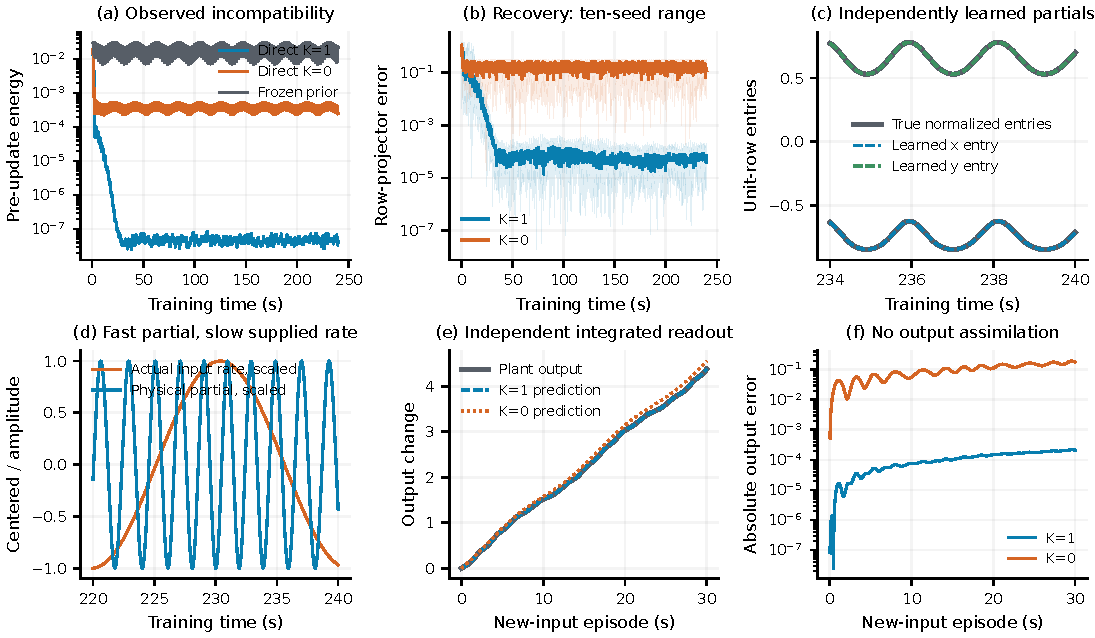
\includegraphics[width=.98\textwidth]{direct_fourier_summary.pdf}
\caption{Current direct Fourier evidence. Panels (a,c--f) use prospectively
selected seed~10; (b) shows the median and full range over all ten seeds.
Panel (a) is a causal 1-s mean of pre-update observed energy. Panel (c)
uses unit/sign alignment only for evaluating the two independently learned
entries. Panel (d) centers the actual input rate and physical partial and
divides each by its amplitude. Panels (e,f) integrate the same learned
readout on a new input, without later output assimilation.}
\label{fig:direct_fourier_new}
\end{figure*}

The final clean coefficient-covariance gap ranges from $.0054964$ to
$.0055467$, and $\|R_{\rm clean}C_*^{\mathsf T}\|$ is at most
$4.13\times10^{-15}$. Noisy covariance spectra and target-memory bias are
saved separately. A positive noisy eigengap is not treated as proof of
physical identification or unbiased recovery. All six coefficient entries
change in every run; the largest unit-norm error is $3.34\times10^{-16}$.
The generic learned field need not itself be a Jacobian. In this graph
geometry, wherever $\widehat H_y\ne0$, the gauge-equivalent field
$\widehat H/\widehat H_y=(\widehat H_x/\widehat H_y,1)$ is the gradient of
$y+\int (\widehat H_x/\widehat H_y)\,dx$. This post hoc interpretation does
not supply a potential to training and does not establish general
high-dimensional integrability.

\paragraph{Prespecification, verification, and provenance.}
The protocol fixed seeds 10--19, illustration seed~10, durations, observations,
initialization, baselines, and criteria before any new run. The excluded
exploratory pilot uses seed~9001. Each confirmatory seed passes the declared
limits: late mean projector error below $.01$, heldout rate RMSE below
$.002$, output RMSE below $.02$, and no learned heldout guard failure. These
are numerical evidence thresholds, not theorem hypotheses or significance
tests. No heldout result was used for tuning, and no run was omitted.

Two predeclared noise-free seed-10 refinements use $\Delta t=.02$ and $.01$~s.
Their final coefficient rows differ by at most $1.15\times10^{-14}$;
rate errors are below $1.84\times10^{-15}$ and integrated-output RMSE decreases
from $4.37321\times10^{-6}$ to $1.09337\times10^{-6}$. Direct projector
subtraction gives late errors below $10^{-14}$. The original equivalent
$\sqrt{2(1-\cos^2\theta)}$ summaries suffer cancellation at this scale and
report about $4\times10^{-9}$; those immutable summaries and the diagnosed
discrepancy are retained. This arithmetic floor is not interpreted as a
physical recovery error. The clean check isolates quadrature and update
accuracy, not a robustness test for noisy derivative estimation.

An independent audit reconstructs every recorded covariance transition,
observation/RNG stream, heldout rate and integrated trajectory. Selected
updates are checked against a tighter direct integration of the full
nonlinear coupled $(C,R)$ equations. All thirteen cases---the ten
confirmatory seeds, pilot, and two refinements---pass. The evaluator slope
is separately checked by finite differences of the simulator graph.
The portable source and commands are under
\path{experiments/direct_submission/fourier/}: \path{run.py},
\path{protocol.json}, \path{audit.py}, \path{summarize_plot.py}, and
\path{REPRODUCE.txt}. Each raw run retains source, configuration, complete
observed rates and pre-update coefficient/covariance states, predictions,
evaluator-only channels, RNG states, environment, and SHA-256 manifest.
The raw evidence archive is identified separately by the accompanying package manifest;
a local package does not imply that it has already been published.
The benchmark supports direct field learning and independent prediction
under known phase/order and the stated sensors. It does not validate the
old periodic plant's control, unknown-frequency discovery, noisy-rate
estimation from position-only sensors, or global stability.

\subsection{Direct local-field contact: protocol, readout, and limitations}
\label{sec:direct_contact_protocol}
The task is to regulate horizontal position $x$ and the vertical force
component $\lambda$ through a material/actuator change. The learner adapts all
$24$ entries of a local $3\times8$ field; its learned relations determine the
input-rate commands. This direct-field study is distinct from the retained
coefficient-family reconstruction and its geometry-dependent normal-force task.

\paragraph{Physical relation and observations}
The simulator uses $\dot p=Bu$, $p=(x,y)^{\mathsf T}$, and
\begin{align}
 \dot\lambda&=a\{h(x)-y\}-4\lambda+b\{h'(x)\dot x-\dot y\},\nonumber\\
 h(x)&=.035\sin2x+.020\cos5x.
 \label{eq:direct_contact_plant}
\end{align}
Initially $(a,b)=(600,240)$ and
$B=\left[\begin{smallmatrix}1&.15\\-.08&.85\end{smallmatrix}\right]$.
At $60$ s they change to $(1000,360)$ and
$B=\left[\begin{smallmatrix}.8&.22\\-.12&.65\end{smallmatrix}\right]$
without informing the learner. The initial state is
$(x,y,\lambda)=(0,.020-4/150,4)$.
The observed context and fixed units are
\begin{align}
 z&=(x,y,\lambda,v_x,v_y,r,u_1,u_2),\quad r=\dot\lambda,\nonumber\\
 D&=\operatorname{diag}(.3,.03,5,.15,.03,5,.15,.03),\quad
 v=D^{-1}\dot z.\label{eq:direct_contact_units}
\end{align}
On each smooth material branch, the plant obeys the three implicit relations
\begin{equation}
 f(z)=\begin{bmatrix}
 r-a\{h(x)-y\}+4\lambda-b\{h'(x)v_x-v_y\}\\
 v_x-B_{11}u_1-B_{12}u_2\\
 v_y-B_{21}u_1-B_{22}u_2
 \end{bmatrix}=0.
 \label{eq:direct_contact_relation}
\end{equation}
Writing $\gamma=a h'(x)+b h''(x)v_x$, the true field $F=D_zf$ is
\begin{equation}
 F=\begin{bmatrix}
 -\gamma&a&4&-b h'(x)&b&1&0&0\\
 0&0&0&1&0&0&-B_{11}&-B_{12}\\
 0&0&0&0&1&0&-B_{21}&-B_{22}
 \end{bmatrix}.
 \label{eq:direct_contact_true_field}
\end{equation}
Thus $F\dot z=0$ relates motion, force variation and actuation. These formulas
are simulator/evaluator-only: neither $f,F$ nor $a,b,B,h$ enters the learner or
controller. Supplied choices are context, units, three-constraint dimension,
initialization, learning settings and task references. A noise-free ideal
sensor supplies $z$ and its physical rate, including force rate and force
acceleration, from forward physics; no differentiation of noisy force data
is tested.

Commands are piecewise linear. At a sample, the observed rate is the left-hand
rate produced by the preceding command slope; the newly computed slope acts
over the next interval. At the material/actuator change, the sensor reports
the new branch's finite one-sided rates. The jump impulse of a discontinuous
context component is not assimilated as an ordinary derivative sample.
This is a piecewise-smooth simulation, not an impact or impulse-observation
model. The state is advanced by RK4 with the interval's appropriate material
branch and linearly varying command.

\paragraph{Direct learning from measured rates}
For seed $s$, a QR factorization of a generic $8\times3$ Gaussian matrix with
RNG seed $s+10000$ gives $Q_0$; $R_0=0$. The learned physical field is
$\widehat F=QD^{-1}$, with incompatibility $Qv=\widehat F\dot z$.
No entry is fixed to zero, one, or a prescribed sign, and no sparsity or
coefficient ties are imposed. The rows are normalized by the executed law:
\begin{align}
 \dot R&=vv^{\mathsf T}-.5R,\qquad QQ^{\mathsf T}=I_3,\nonumber\\
 \dot Q&=-100\{QR-(QRQ^{\mathsf T})Q\}.
 \label{eq:direct_contact_law}
\end{align}
At each $0.01$-s sample, the pre-update $Q$ forms the command and scores the
observed incompatibility. The current observed $v$ is then held during the
learning interval. Its covariance is integrated exactly as
$R(s)=e^{-.5s}R_n+2(1-e^{-.5s})v_nv_n^{\mathsf T}$, and DOP853 integrates
$Q$ against this evolving covariance, with relative/absolute tolerances
$10^{-10}/10^{-12}$. An endpoint polar correction removes numerical drift;
a raw orthogonality error greater than $10^{-7}$ aborts the run. An
instantaneous eigensolver is not substituted for the learning dynamics.
The evaluator obtains physical partials only after command construction.
Learning remains active for all $120$ s; at $40$ s, open-loop probing gives
way to feedback control.

\paragraph{Comparing learned and true partial relations}
Row-space agreement is measured in the fixed units by
$e_P=\|Q^{\mathsf T}Q-T^{\mathsf T}T\|_F$, where
$T=\{(FD)(FD)^{\mathsf T}\}^{-1/2}FD$ is the orthonormal true row frame.
For entrywise comparison, if $TQ^{\mathsf T}=U\Sigma V^{\mathsf T}$,
compare $OQ$ with $T$, where $O=UV^{\mathsf T}$ is evaluator-only.
This orthogonal alignment preserves column norms and row-space geometry,
not individual entry amplitudes. It does not enter learning or control;
the comparison concerns normalized partial relations, not unique canonical
values of $F$. For seed $101$ during control,
$\min\sigma(TQ^{\mathsf T})=.940553$; the orthogonal-factor error is below
$3.1\,10^{-15}$. The actual learned control block has minimum singular value
$.054216$, compared with $.127422$ for the orthonormal physical control block.
Small incompatibility is not reported as exact physical identification.

Canonical normalization fixes the $(r,u_1,u_2)$ columns $(6,7,8)$ by
inverting their unscaled learned block, whose minimum singular value reaches
$6.06\,10^{-6}$. This poorly conditioned inversion can produce inaccurate
material entries (Fig.~\ref{fig:direct_contact_canonical}). The controller
instead supplies $\dot r$ and solves the scaled $(v_y,u_1,u_2)$ block
$(5,7,8)$ for $(\dot v_y,\dot u_1,\dot u_2)$. Its regular completion can
therefore support useful regulation while the different canonical inversion
amplifies field errors. The evidence supports approximate local row-space
tracking, not precise material magnitudes, global integrability, or
unrestricted plant identification.
For seed $101$ in the primary window, the empirical bottom-three memory
subspace has mean projector distance $.28834$ from the physical row space,
while the learner--memory distance is $.09478$ and the third/fourth eigengap
is $.0003995$. These distinct diagnostics expose local-history bias and
tracking lag, rather than interpreting covariance positivity as physical
persistent excitation.

\begin{figure*}[p]
\centering
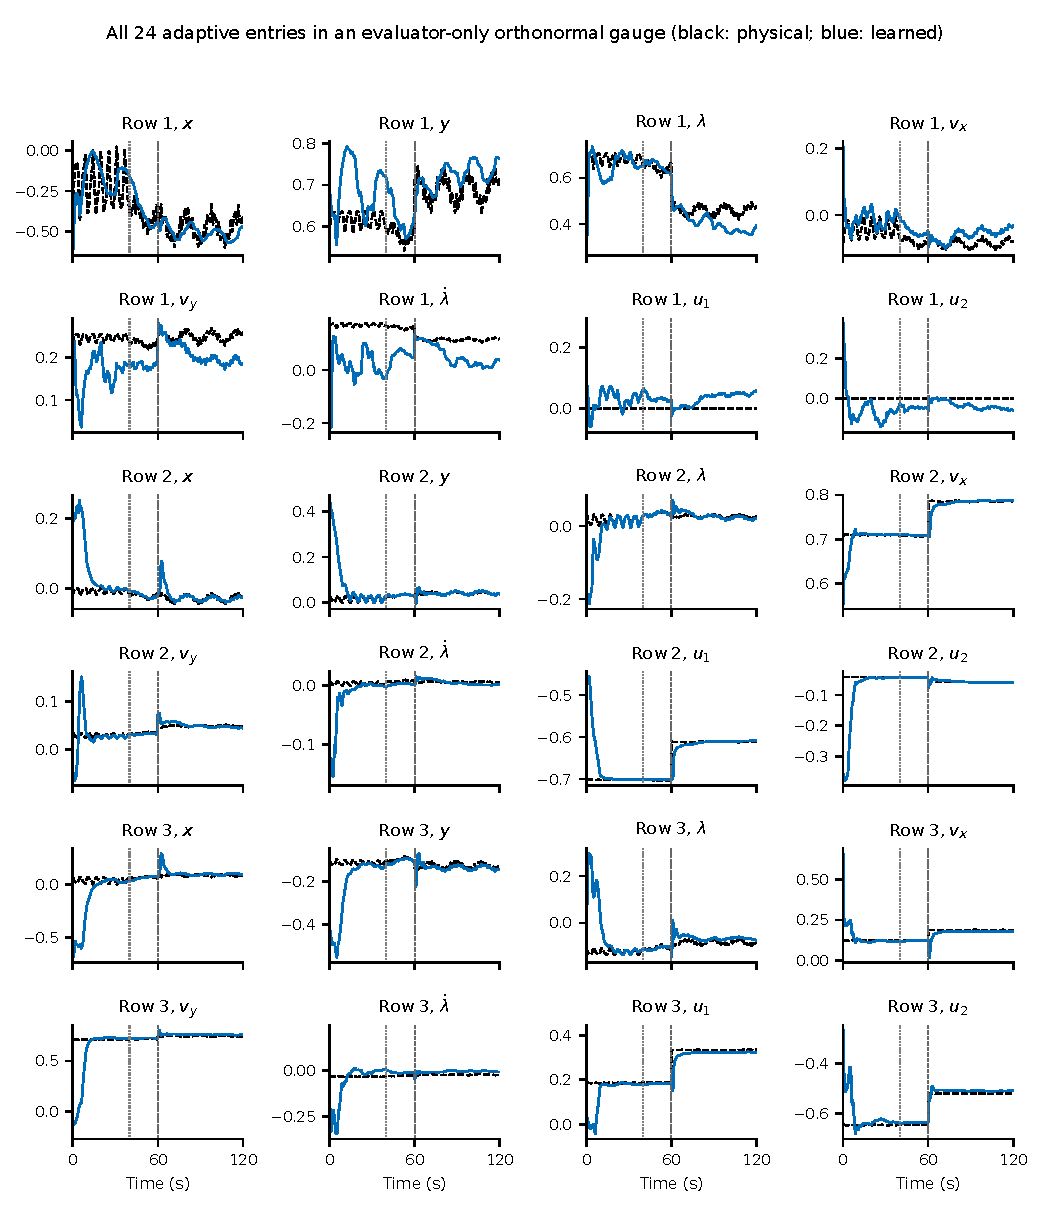
\includegraphics[width=\textwidth]{figures/direct_contact_all24.pdf}
\caption{Learning the contact relation: all $24$ adaptive entries for
preselected seed $101$. Each panel compares the same entry of the normalized
true field $T$ (black dashed) and aligned estimate $OQ$ (blue), using the
fixed units and evaluator-only orthogonal alignment defined in the text.
The learner receives no entries of $F$. Open-loop probing ends and control
begins at $40$ s (dotted line); learning continues throughout all $120$ s.
The material/actuator change occurs at $60$ s (dashed line).
Residual discrepancies remain visible; task success is not exact recovery
of every physical partial.}
\label{fig:direct_contact_all24}
\end{figure*}
\begin{figure}[t]
\centering
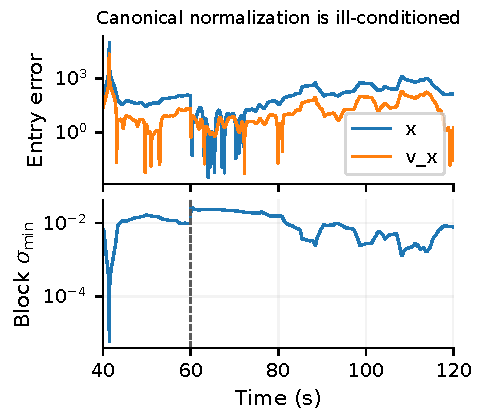
\includegraphics[width=\columnwidth]{figures/direct_contact_canonical_gauge_limitation.pdf}
\caption{A retained limitation: normalizing the material force-rate entry to
one is poorly conditioned and yields large physical-entry errors. This
normalization is evaluator-only and never used for commands or learning.}
\label{fig:direct_contact_canonical}
\end{figure}

\paragraph{Feedback and learned-field readout}
A measured open-loop warmup occupies $0\le t<40$ s:
\begin{align}
 u_1(t)&=.06\sin1.1t+.03\sin(2.3t+.4)\nonumber\\
       &\quad+.015\sin(3.7t+.2),\nonumber\\
 u_2(t)&=.002\sin(.9t+.8)+.0015\sin1.9t\nonumber\\
       &\quad+.001\sin(3.1t+.1).
 \label{eq:direct_contact_probe}
\end{align}
The applied warmup slope is the forward difference of these prescribed input
values across the next sample interval. This is an ordinary observed temporal
trajectory, not a source of independently labeled perturbation tangents.
After warmup, with $s=t-40$, the references are
\begin{align}
 x_d&=.03\sin(.35s)+.01\sin(2.3s)+.005\sin(3.7s),\nonumber\\
 \lambda_d&=4+.2\sin(.5s)+.08\sin(1.9s)+.04\sin(3.1s).
 \label{eq:direct_contact_reference}
\end{align}
Their derivatives are known task inputs; small independent components maintain
local excitation. Feedback prescribes $\dot v_x=a_x^*$ and
$\dot r=a_\lambda^*$:
\begin{align}
 a_x^*&=\ddot x_d-4(v_x-\dot x_d)-4(x-x_d),\nonumber\\
 a_\lambda^*&=\ddot\lambda_d-6(\dot\lambda-\dot\lambda_d)
                         -9(\lambda-\lambda_d).
 \label{eq:direct_contact_feedback}
\end{align}
The supplied rates are $(v_x,v_y,r,a_x^*,a_\lambda^*)$; the computed
rates are $(a_y,\dot u_1,\dot u_2)$. Using one-based columns
$S=(1,2,3,4,6)$ and $C=(5,7,8)$, the same pre-update relation
$\widehat F\dot z=0$ gives
\begin{equation}
 \begin{bmatrix}a_y\\\dot u_1\\\dot u_2\end{bmatrix}
 =-D_CQ_C^{-1}Q_SD_S^{-1}
 \begin{bmatrix}v_x\\v_y\\r\\a_x^*\\a_\lambda^*\end{bmatrix}.
 \label{eq:direct_contact_completion}
\end{equation}
Desired rates enter this query only; learning still uses observed $v$.
Only the last two completed components are applied: their limited slopes
update the measured input by $u_{n+1}=u_n+\Delta t\,\dot u_n$.
The inferred $a_y$ closes the relation but is not a separate actuator command.
Limits are $|u_i|\le.8$ and $|\dot u_i|\le5$.
If $\sigma_{\min}(Q_C)<.005$, the trajectory is recorded as failed and stops;
there is no physical inverse or fallback controller. Domain checks stop a run
if indentation or force is nonpositive, $|x|>1$, $|y|>.3$, or $|\lambda|>100$.
The prescribed control law contains neither $a,b,B$ nor $h$.

\paragraph{Task results and retained failures}
Exploratory seed $0$ was separate from confirmation. Its first, less excited
reference reached a readout guard at $58.58$ s and is retained as a failure.
The local references in~(\ref{eq:direct_contact_reference}) completed both a
60-s constant-plant pilot and a 120-s pilot with the scheduled change.
The learning gain, memory, units, and guard were unchanged. The measured
conditioning and task response motivated the reference revision; physical
partial errors were not feedback or selection inputs.

The complete protocol and source hashes were fixed before seeds
$101$--$105$, with seed $101$ preselected for illustrations. These seeds vary
generic field initialization; they are not five independently drawn plants or
noise realizations. The declared primary window was $[110,120)$ s. Criteria
required complete 120-s trajectories, no domain/guard/saturation event,
position RMSE below $.01$, vertical-force RMSE below $.2$, mean row-projector
error below $.6$, and field, incompatibility, and query errors below half their
respective frozen-initial same-stream values. All five runs met these
criteria; no seed was discarded.

\begin{table}[t]
\centering\small\setlength{\tabcolsep}{2.5pt}
\caption{All declared direct-contact runs, primary window $[110,120)$ s.
$e_P=\|Q^{\mathsf T}Q-P_{FD}\|_F$ in the fixed units of
(\ref{eq:direct_contact_units}). Query error is RMS norm over all three
completed physical rates. The frozen estimate is a same-stream shadow.}
\label{tab:direct_contact_seeds}
\begin{tabular}{rccccc}
\hline
Seed & Force RMSE & Position RMSE & Mean $e_P$ & Query RMS & Pass\\
\hline
101 & .121637 & $6.8111\,10^{-5}$ & .298169 & .00717262 & Yes\\
102 & .121637 & $6.8110\,10^{-5}$ & .298169 & .00717265 & Yes\\
103 & .121636 & $6.8112\,10^{-5}$ & .298169 & .00717260 & Yes\\
104 & .121642 & $6.8105\,10^{-5}$ & .298170 & .00717283 & Yes\\
105 & .121636 & $6.8113\,10^{-5}$ & .298169 & .00717260 & Yes\\
\hline
\end{tabular}
\end{table}
Across the five seeds, force RMSE is $.121638\pm2.31\,10^{-6}$,
position RMSE is $(6.81102\pm.00031)10^{-5}$, and mean projector error is
$.298169\pm6.15\,10^{-7}$ (sample standard deviations). The frozen projector
error is $1.93389\pm.16981$. Mean incompatibility norm is $.00359588$ versus
$.511730$ for frozen initialization. Query RMS is $.00717266\pm9.66\,10^{-8}$
versus $.214812\pm.100090$ for the frozen shadow. Query comparison supplies
the same requested rates to the learned and physical fields; it is an
inverse-readout diagnostic, not an independent future-prediction experiment.
Own-trajectory force/motion errors separately test the applied readout.

\paragraph{Numerical and provenance checks}
Saved records include every pre-update $Q,R,z,\dot z$, command, supplied query,
physical evaluator field, source snapshot, configuration, and per-file hash.
Recalculation from raw records reproduced trace metrics and controller outputs.
The covariance transition error is at most $1.12\,10^{-14}$; independent
200-substep RK4 checks of selected learning intervals agree within
$2.57\,10^{-12}$ in $Q$. Every entry changed, with the smallest across-entry
maximum change exceeding $.1185$ over the audited runs. Directional finite
differences check the evaluator partials separately from the learning rule.

The predeclared seed-$101$ refinement halves the observation/plant step to
$.005$ s, with all other settings unchanged. It also completes and passes the
criteria. Its force RMSE is $.109237$, versus $.121637$ at $.01$ s; projector
error is $.297450$, versus $.298169$. The same-time late force trajectories
differ by RMS $.01490$ N, and projector-error traces by RMS $.001719$.
Thus qualitative success is preserved, but fine quantitative force accuracy
is discretization-sensitive; the coarse records have not been replaced or
called a converged continuous-time solution.

The portable implementation, frozen protocol, auditing and plotting programs
are under \texttt{experiments/direct\_submission/contact/}. This new identity
has nine recorded executions: three exploratory cases, five confirmation
seeds, and one refinement. The earlier experiments using noisy measured
signals and cascaded causal differentiation are different protocols; their
failures remain archived and do not establish robustness for this study.
Local records and hashes are evidence of execution,
not a claim that a new archive or code revision has already been published.

\subsection{Direct five-entry Burgers learning and distributed readout}
\label{sec:direct_burgers_protocol}

This experiment replaces the prescribed three-coefficient Burgers learner in
its role as main-paper evidence. The earlier coefficient-family experiment
remains a separate historical protocol. Here every entry of a local differential
row is learned directly from observed context-rate incompatibility; the physical
Burgers coefficient family is used only to generate and evaluate the plant.
The protocol was fixed before running the five initializations and subsequent
sensor and timestep conditions. The main figure uses the preselected seed 732
and spatial site 0, without selection by the outcome.

\subsubsection{Plant, observations, and free differential row}
On the periodic domain $s\in[0,2\pi)$, the simulator is
\begin{equation}
 w_t+w w_s-.08w_{ss}-u=0,
 \qquad z=(w,w_s,w_{ss},u,w_t).
 \label{eq:direct_burgers_plant}
\end{equation}
A 32-point Fourier collocation grid and RK4 advance the physical state with
piecewise-linear $u$. All spatial points are sensed and actuated. The initial
state is $w(s,0)=.2+.015\sin s$, with $u(s,0)=0$. Fixed identity context scales
are used. At each site the learner stores an independent row
$q\in\mathbb R^{1\times5}$ and a $5\times5$ memory matrix. Every entry of $q$
is initialized from a generic Gaussian draw, followed by unit normalization.
The five initial seeds are 732--736; the independent sensor seed is the initial
seed plus 100000. No coefficient estimate, known partial entry, sparse physical
pattern, physical eigenspace, or true-$F$ initialization is supplied.

In the ideal condition, $w$ and $w_t$ are measured exactly; spatial channels
are spectral derivatives of the measured field. This is an explicit ideal
sensor assumption, not a noisy position-only result. The learner does not
receive an exact $w_{tt}$ sensor: its observation is the causal context secant
\begin{equation}
 v_k=\frac{z(t_k)-z(t_k-.05)}{.05},\qquad t_{k+1}-t_k=.005\,\mathrm{s}.
 \label{eq:direct_burgers_observation}
\end{equation}
After the first valid history window, it integrates
\begin{equation}
 \begin{aligned}
 \dot R&=v_kv_k^T-R/4,\\
 \dot q&=-10^4\{qR-(qRq^T)q\},\qquad qq^T=1.
 \end{aligned}
 \label{eq:direct_burgers_law}
\end{equation}
The secant is held during the current $.005$-s observation interval, but the
memory evolves throughout the representation update. Each RK4 stage evaluates
\begin{equation}
 R(t_k+\delta)=e^{-\delta/4}R_k+
               4(1-e^{-\delta/4})v_kv_k^T.
 \label{eq:direct_burgers_memory}
\end{equation}
At least four subdivisions are used; their length $d$ obeys
$10^4d\max\{\operatorname{tr}R_k,\operatorname{tr}R_{k+1}\}\leq.25$
across sites. Unit normalization follows each subdivision. This is numerical
integration of the coupled law, not replacement of learning by a bottom
eigenvector or descent with a frozen memory matrix.

\subsubsection{Training and same-field rate completion}
For $0\leq t<80$ s the input-rate probe is
\begin{equation}
 \begin{aligned}
 \dot u&=.01\sum_{k=0}^{3}\omega_k
       \sin((k+1)s+.37k)\cos(\omega_kt),\\
 &(\omega_0,\ldots,\omega_3)=(3,5,7,11).
 \end{aligned}
 \label{eq:direct_burgers_probe}
\end{equation}
Before observing $t=80$ s, the complete plant, input, learned row, memory,
observation histories and random-number state are cloned. One arm continues
learning and the other holds $q$ fixed. Both act on their own physical
trajectories until $t=100$ s. The fixed arm may evolve a diagnostic memory;
that memory does not update its row.

The target is
\begin{equation}
 w_d=.2+.015\sin s\cos(.3t)+.01\cos(2s)\sin(.5t).
 \label{eq:direct_burgers_reference}
\end{equation}
At each controlled sample, measured channels and the pre-update row form the
query before the current secant is assimilated. Set
\begin{equation}
 a_d=(w_d)_{tt}-4(w-w_d)-4(w_t-(w_d)_t).
\end{equation}
The supplied rates are $v_S=(w_t,(w_t)_s,(w_t)_{ss},a_d)$ and the computed
channel is $v_C=\dot u$. The same learned row returns
\begin{equation}
 \dot u=-\frac{q_w w_t+q_{w_s}(w_t)_s+q_{w_{ss}}(w_t)_{ss}+q_{w_t}a_d}{q_u}.
 \label{eq:direct_burgers_completion}
\end{equation}
A query with $|q_u|<.1$ uses the declared model-independent input decay $-u$
and is counted as guarded, not successful learned completion. Applied input
rates are clipped to $[-5,5]$; $\max_s|w|>5$ stops a branch. There is no
physical-model fallback. The ideal cohort has no guarded or clipped controlled
sample and no stopped branch; its smallest controlled $|q_u|$ is $.67137$.

\subsubsection{Separate recovery, compatibility, and task scores}
Only the evaluator forms the physical row
$F=(w_s,w,-.08,-1,1)$ at each branch's actual clean context. Let
$p=F/\|F\|$. The physical recovery metric is
\begin{equation}
 e_F=\|q^Tq-p^Tp\|_F=\sqrt{2(1-(qp^T)^2)}.
 \label{eq:direct_burgers_score}
\end{equation}
It is invariant to row sign and scale and ranges from zero to $\sqrt2$.
Entry plots use unit normalization and evaluator-only sign alignment; this
display convention never changes the learner or controller. Pre-update
incompatibility is scored separately as $\frac12(qv_k)^2$. Task RMS is the
root mean square of $w-w_d$ over all sites and applied observations in the
specified window. Terminal commands at $t=100$ are stored but not applied and
are excluded from task/readout metrics. Rendering uses every fifth sample;
metrics use every applied sample without smoothing.

\begin{figure}[t]
 \centering
 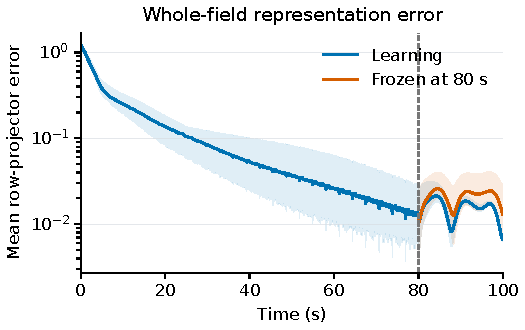
\includegraphics[width=\columnwidth]{figures/direct_burgers_diagnostics.pdf}
 \caption{Whole-field Burgers representation error, complementing the main
figure's partial, incompatibility and control plots. Curves are means and bands
span all five seeds, with error averaged over all 32 spatial sites. At 80 s,
the shared probing trajectory branches into separately controlled adaptive
and frozen runs. The adaptive rows continue learning through 100 s;
the frozen rows retain their values at 80 s.}
\label{fig:direct_burgers_protocol}
\end{figure}

\begin{table*}[t]
\centering
\caption{All ideal main-cohort outcomes. Late means/RMS use $[96,100)$ s.
The training qualification uses $[76,80)$ s and all the criteria stated in the text.
The final row gives the across-seed mean $\pm$ sample standard deviation.}
\label{tab:direct_burgers_ideal}
\renewcommand{\arraystretch}{1.15}
\begin{tabular}{c c c c c c}
\hline
Seed & Training qualified & Adaptive $e_F$ & Frozen $e_F$ &
Adaptive task RMS ($10^{-6}$) & Frozen task RMS ($10^{-6}$)\\
\hline
732 & No & .013761 & .018433 & 8.5084 & 22.4895\\
733 & No & .013222 & .021239 & 8.5186 & 25.8758\\
734 & Yes & .013231 & .014272 & 8.4460 & 11.7942\\
735 & No & .014729 & .037314 & 8.9005 & 49.9873\\
736 & Yes & .013344 & .015503 & 8.4874 & 13.9083\\
\hline
All five & 2/5 & $.013658\pm.000638$ & $.021352\pm.009323$ &
$8.5722\pm.1856$ & $24.8110\pm15.2371$\\
\hline
\end{tabular}
\end{table*}

The prospective training qualification requires mean $e_F\leq.05$, pooled
95th percentile $\leq.1$, maximum $\leq.25$, worst-site mean $\leq.1$, and
mean error at most one quarter of the initial-row same-stream error. Only
seeds 734 and 736 pass every condition. All five pass the inherited weaker
mean/reduction check and all five pass the declared adaptive late conditions:
mean $e_F\leq.1$, 95th percentile $\leq.25$, task RMS $\leq10^{-3}$,
guard and clipping fractions each strictly below $.01$, and completion to
100 s. These are offline labels, never training stops or feedback gates.
The five-seed result therefore demonstrates continued direct learning and
readout, not uniformly qualified tracking after convergence.

Over the full $[80,100)$ control interval, adaptive and frozen task RMS are
$.001223645\pm.000000231$ and $.001223943\pm.000000617$, respectively.
Their common initial transition dominates this interval; the late advantage
must not be described as a large full-horizon improvement. For the two
qualified seeds, frozen readout already works well and continued learning
provides a modest late improvement. The remaining seeds include continuing
recovery from incomplete training.

Even ideal sensing does not make the finite secant exactly tangent to the
instantaneous physical relation. The physical unit-row half-mean-square
secant energy is $4.4414\times10^{-11}$ over $[76,80)$ and averages
$1.5610\times10^{-13}$ on the adaptive late trajectories. The latter learned
energy is $3.6992\times10^{-10}$. Thus neither numerical zero compatibility
nor exact physical identification is claimed. The local time-varying rows
need not define an integrable global Jacobian field.

\subsubsection{Sensor failures and numerical refinement}
The complete study retains 19 cases: five ideal, five causal-clean and five
causal-noisy main cases, plus two ideal and two causal-clean refinements.
In causal cases a quadratic endpoint least-squares fit to the preceding $.10$
s of measured positions estimates $w_t$; the same estimate supplies both the
context and controller. No future samples or true-rate fill are used. Noisy
cases add independent position noise with standard deviation $10^{-5}$ per
site/sample. The causal secant first becomes valid at $.15$ s. Noise and row
initializations vary together across the five paired seeds; this is not a
crossed factorial noise study.

\begin{table}[t]
\centering
\caption{Main-cohort outcomes, retaining every seed. ``Late pass'' requires
all combined adaptive recovery, task, guard and completion criteria.}
\label{tab:direct_burgers_conditions}
\renewcommand{\arraystretch}{1.15}
\begin{tabular}{lccc}
\hline
Sensing & Training qualified & Late pass & Complete A/F\\
\hline
Ideal & 2/5 & 5/5 & 5/5, 5/5\\
Causal clean & 0/5 & 0/5 & 5/5, 0/5\\
Causal noisy & 0/5 & 0/5 & 5/5, 5/5\\
\hline
\end{tabular}
\end{table}

Every causal-clean frozen main branch reaches the declared field bound at
83.2 s. The two causal-clean frozen refinements stop at 83.2 and 83.2025 s.
Failed observations and unexecuted commands remain in the raw records; absent
late windows are not extrapolated. The causal-clean training discrepancy is
principally a biased observed covariance target: for seed 732 the learned,
observed-bottom and clean-bottom physical errors are $.479532$, $.480820$
and $.004098$, respectively. Small observed incompatibility does not identify
the physical partials. In the noisy cohort, adaptive late mean physical error
is $1.41362$, task RMS is $.007956$, and the guard fraction is one. Continued
adaptation under that sensor model is not successful partial recovery.

For preselected seed 732, the whole-loop step is halved from $.005$ to $.0025$
and $.00125$ s, keeping physical windows fixed. Ideal late mean field changes
are $2.11605\times10^{-5}$ and $9.60095\times10^{-6}$; the first exceeds the
prospective absolute $10^{-5}$ sensitivity flag, while neither exceeds the
10\% relative flag. Worst-site training means $.104301$, $.100618$ and
$.098807$ cross the qualification boundary only at the finest step. That
favorable result does not replace the prespecified main-cohort count of 2/5.
The second causal-clean halving changes late field error by 18.70\% and task
RMS by 38.39\%, so its whole-loop sensitivity test fails. Halving the loop
changes sensing, sampling and control as well as integration; it is not a
pure solver-order or continuous-PDE convergence test.

\subsubsection{Reproduction and audit boundary}
The portable package is
\path{experiments/direct_submission/burgers/}.
Its \path{protocol.json} preserves the original prospective declaration;
\path{source_mapping.json} distinguishes unchanged scientific functions from
local import, command-line and provenance adaptations. The package includes
compact full-sample plot trajectories, selected complete original chunks and
checkpoints, and all-condition summaries. These selected files are not the
complete 6.63-GB original raw archive, which remains a separate artifact;
no public download location is implied here.

The independent final-pass reconstruction checks the hashes of all 610 ideal
raw chunks and reproduces 200 metric comparisons. Every controlled command
is reconstructed from the saved pre-update row and observed supplied rates;
the largest discrepancy is $1.39\times10^{-17}$. Portable-source replay of
600 archived samples across training, adaptive and frozen phases is bitwise
identical. An independent literal joint-$q/R$ ODE check gives a row discrepancy
$1.51\times10^{-10}$, with successive held-observation halving errors
$9.29\times10^{-12}$ and $5.77\times10^{-13}$. The historical independent
audit also retains all 19 cases, sensor/filter reconstruction, coupled-ODE
checks and failed branch records.

From the package directory, \path{verify_package.py} performs the focused
replay/numerical checks, \path{plot_figure_focus.py} regenerates the current
figures without simulation, \path{burgers_direct.py} reproduces one declared case or the complete
study in a new directory, and \path{audit_runs.py} independently reconstructs
raw runs without importing the learner or simulator. The README gives exact
commands and dependencies. These numerical checks verify implementation and
provenance; they do not establish global identifiability, sensor robustness,
off-trajectory integrability or closed-loop stability.


\subsection{Records, reproduction, and release identity}
The direct-study package contains independent executable subdirectories for
\path{fourier/}, \path{contact/}, and \path{burgers/}, their declared
protocols, and commands to reproduce into new output directories. The final
package manifest binds source hashes, figure inputs, compact replay data,
and complete raw-data archives. Original run records are immutable; display
or packaging corrections create separate analysis artifacts. The Burgers
portable wrapper changes import/command-line/provenance plumbing only;
its scientific functions and native numerical kernel are checked against
the executed sources.

Every seed and failed query is retained. Fourier and contact pilot records
are identified as exploratory and excluded from confirmation statistics.
Contact's first pilot fails its query guard; the later reference protocol
was fixed before the five new initializations. The Burgers ideal cohort is
not a newly rerun favorable subset: all 19 declared cases, including failed
sensing challenges and numerical refinements, remain reported together.
These disclosures preserve the distinction between a successful scoped
simulation, exploratory design, and broad robustness evidence.

The local package accompanies the revised documents. No claim that its
current revision is already a public GitHub release or permanent external
archive is made. Full raw data have separate checksums from compact
reproduction/figure records and from every earlier structured-study archive.


\bibliographystyle{IEEEtran}
\bibliography{references}
\end{document}
